%   author: samtenka
%   change: 2020-07-25
%   create: 2020-07-19
%   descrp: LaTeX source for perturb project, SM thesis writeup
%   to use: compile along with perturb.bib and diagram and plot directories

%==============================================================================
%=====  LATEX PREAMBLE  =======================================================
%==============================================================================

%~~~~~~~~~~~~~~~~~~~~~~~~~~~~~~~~~~~~~~~~~~~~~~~~~~~~~~~~~~~~~~~~~~~~~~~~~~~~~~
%~~~~~~~~~~~~~  Document Styling  ~~~~~~~~~~~~~~~~~~~~~~~~~~~~~~~~~~~~~~~~~~~~~

\documentclass[openany, notitlepage, justified]{tufte-book}
%\usepackage{geometry}
\usepackage[utf8]{inputenc}
\usepackage[T1]{fontenc}
\usepackage{microtype}      
\usepackage{datetime}      
\usepackage{listings}      
\usepackage{epigraph}      

\geometry{
    height=11.0in,
    width=8.5in,
    left=1in, % left margin
    textwidth=4.6in, % main text block
    marginparsep=0.2in, % gutter between main text block and margin notes
    marginparwidth=1.7in % width of margin notes
}

\usepackage{natbib}
\setcounter{secnumdepth}{1}
%\usepackage{setspace}
%\doublespacing

%---------------------  mathematics  ------------------------------------------

\usepackage{amsmath, amssymb, amsthm, amsfonts}
\usepackage{mathtools, nicefrac, xstring, enumitem}

\usepackage{setspace}
%---------------------  tables  ----------------------------------------------- 

\usepackage{booktabs}
\usepackage{array}
\newcolumntype{L}{>{$}l<{$}}

%---------------------  graphics and marginfigures  ---------------------------------

\usepackage{graphicx}
\usepackage{wrapfig, float}
\usepackage{hanging, txfonts, ifthen}

\newcommand{\moolor}[2]{\par\hrulefill\\#2\vspace{#1 cm}\par\hrulefill\\}

\newcommand{\ofsix}[1]{
    {\tiny \raisebox{0.04cm}{$\substack{
        \ifthenelse{\equal{#1}{0}}{{\color{moor}\blacksquare}}{\square}
        \ifthenelse{\equal{#1}{2}}{{\color{moor}\blacksquare}}{\square}    
        \ifthenelse{\equal{#1}{4}}{{\color{moor}\blacksquare}}{\square} \\
        \ifthenelse{\equal{#1}{1}}{{\color{moor}\blacksquare}}{\square}    
        \ifthenelse{\equal{#1}{3}}{{\color{moor}\blacksquare}}{\square}
        \ifthenelse{\equal{#1}{5}}{{\color{moor}\blacksquare}}{\square}
    }$}}%
}

\newcommand{\offive}[1]{
    {\tiny
        \raisebox{-0.04cm}{\color{gray}\scalebox{2.5}{$\substack{
            \ifthenelse{\equal{#1}{0}}{{\color{moor}\blacksquare}}{\square} 
        }$}}%
        \raisebox{0.04cm}{$\substack{
            \IfSubStr{#1}{1}{{\color{moor}\blacksquare}}{\square}   
            \IfSubStr{#1}{1}{{\color{moor}\blacksquare}}{\square} \\
            \IfSubStr{#1}{2}{{\color{moor}\blacksquare}}{\square}    
            \IfSubStr{#1}{2}{{\color{moor}\blacksquare}}{\square}    
        }$}%
    }%
}

\newcommand{\offour}[1]{
    {\tiny
        \raisebox{0.04cm}{$\substack{
            \IfSubStr{#1}{0}{{\color{moor}\blacksquare}}{\square}   
            \IfSubStr{#1}{0}{{\color{moor}\blacksquare}}{\square} \\
            \IfSubStr{#1}{1}{{\color{moor}\blacksquare}}{\square}    
            \IfSubStr{#1}{1}{{\color{moor}\blacksquare}}{\square}    
        }$}%
    }%
}

\newcommand{\ofthree}[1]{
    {\tiny \raisebox{0.04cm}{$
        \ifthenelse{\equal{#1}{0}}{{\color{moor}\blacksquare}}{\square}
        \ifthenelse{\equal{#1}{1}}{{\color{moor}\blacksquare}}{\square}    
        \ifthenelse{\equal{#1}{2}}{{\color{moor}\blacksquare}}{\square}
    $}}%
}

\newcommand{\oftwo}[1]{%
    {\tiny\raisebox{0.04cm}{$%
        \ifthenelse{\equal{#1}{0}}{{\color{moor}\blacksquare}}{\square}%
        \ifthenelse{\equal{#1}{1}}{{\color{moor}\blacksquare}}{\square}%   
    $}}%
}


%---------------------  colors  -----------------------------------------------

\usepackage{xcolor, framed}
\definecolor{moolime}{rgb}{0.90,1.00,0.90}
\definecolor{moosky}{rgb}{0.90,0.90,1.00}
\definecolor{moopink}{rgb}{1.00,0.90,0.90}
\definecolor{moor}{rgb}{0.8,0.2,0.2}
\definecolor{moog}{rgb}{0.2,0.8,0.2}
\definecolor{moob}{rgb}{0.2,0.2,0.8}
\definecolor{mooteal}{rgb}{0.1,0.6,0.4}

%---------------------  intertext: footnotes and hyperlinks  ------------------ 

%\usepackage[perpage]{footmisc}
\renewcommand*{\thefootnote}{
    \color{red}
    %\arabic{footnote}
    \fnsymbol{footnote}
} 
%\makeatletter
%    \def\thempfn{\fnsymbol{\@mpfn}}
%\makeatother
\usepackage{perpage}
\MakePerPage{footnote}

\makeatletter
\def\@fnsymbol#1{%
  \ensuremath{%
    \ifcase#1\or
      *\or
      \dagger\or
      \ddagger\or
      \mathsection\or
      \mathparagraph\or
      \|\or
      **\or
      \dagger\dagger\or
      \ddagger\ddagger\or
      \mathsection\mathsection\or
      \mathparagraph\mathparagraph\or
      \|\|\or
      ***\or
      \dagger\dagger\dagger\or
      \ddagger\ddagger\ddagger\or
      \mathsection\mathsection\mathsection\or
      \mathparagraph\mathparagraph\mathparagraph\or
      \|\|\|
    \else
      % We've run out of footnote symbols for this page.
      % We would normally emit an error here,
      % but because the perpage package won't work until the
      % second pass, we need to do something less abrupt.
    \fi
  }%
}
\makeatother

\usepackage{hyperref}

%~~~~~~~~~~~~~~~~~~~~~~~~~~~~~~~~~~~~~~~~~~~~~~~~~~~~~~~~~~~~~~~~~~~~~~~~~~~~~~
%~~~~~~~~~~~~~  Theorem Environments  ~~~~~~~~~~~~~~~~~~~~~~~~~~~~~~~~~~~~~~~~~

%---------------------  mathematical results  ---------------------------------

\theoremstyle{plain}
    \newtheorem*{klem*}{Key Lemma}
    \newtheorem{lem}{Lemma}
    \newtheorem{thm}{Theorem}
    \newtheorem*{thm*}{Theorem}
    \newtheorem{cor}{Corollary}
    \newtheorem{prop}{Proposition}

%---------------------  mathematical questions  -------------------------------

    \newtheorem{conj}{Conjecture}
    \newtheorem{quest}{Question}
    \newtheorem*{quest*}{Question}
    \newtheorem*{quests*}{Questions}

%---------------------  definitions, answers, remarks  ------------------------

\theoremstyle{definition}
    \newtheorem{defn}{Definition}
    \newtheorem*{answ*}{Answer}
    \newtheorem{rmk}{Remark}
    \newtheorem*{midea*}{Main Idea}
    \newtheorem*{rmk*}{Remark}
    \newtheorem{exm}{Example}

%~~~~~~~~~~~~~~~~~~~~~~~~~~~~~~~~~~~~~~~~~~~~~~~~~~~~~~~~~~~~~~~~~~~~~~~~~~~~~~
%~~~~~~~~~~~~~  Custom Math Commands  ~~~~~~~~~~~~~~~~~~~~~~~~~~~~~~~~~~~~~~~~~

%---------------------  expanding containers  ---------------------------------

\newcommand{\wrap}[1]{\left(#1\right)}
\newcommand{\wasq}[1]{\left[#1\right]}
\newcommand{\wang}[1]{\left\langle#1\right\rangle}
\newcommand{\wive}[1]{\left\llbracket#1\right\rrbracket}
\newcommand{\worm}[1]{\left\|#1\right\|}
\newcommand{\wabs}[1]{\left|#1\right|}
\newcommand{\wurl}[1]{\left\{#1\right\}}

\newcommand{\partitionbox}[1]{
    \text{
        \fboxsep=0.5pt
        \tiny
        \fbox{#1}
    }
}

%---------------------  special named objects  --------------------------------

\newcommand{\Free}{\mathcal{F}}
\newcommand{\Forg}{\mathcal{G}}
\newcommand{\Mod}{\mathcal{M}}
\newcommand{\argmin}{\text{\textnormal{argmin}}}
\newcommand{\Hom}{\text{\textnormal{Hom}}}
\newcommand{\Aut}{\text{\textnormal{Aut}}}
\newcommand{\image}{\text{\textnormal{im}}}
\newcommand{\uvalue}{\text{\textnormal{uvalue}}}
\newcommand{\rvalue}{\text{\textnormal{rvalue}}}
\newcommand{\edges}{\text{\textnormal{edges}}}
\newcommand{\ords}{\text{\textnormal{ords}}}
\newcommand{\parts}{\text{\textnormal{parts}}}
\newcommand{\SGD}{\text{\textnormal{SGD}}}
\DeclareMathOperator*{\Avg}{\text{\sffamily A}}
\newcommand{\expc}{\mathbb{E}}
\newcommand{\expct}[1]{\mathbb{E}\left[#1\right]}

%---------------------  fancy letters  ----------------------------------------

\newcommand{\Aa}{\mathcal{A}}
\newcommand{\Bb}{\mathcal{B}}
\newcommand{\Cc}{\mathcal{C}}   \newcommand{\CC}{\mathbb{C}}
\newcommand{\Dd}{\mathcal{D}}
\newcommand{\Ee}{\mathcal{E}}   \newcommand{\EE}{\mathbb{E}}
\newcommand{\Ff}{\mathcal{F}}
\newcommand{\Gg}{\mathcal{G}}
\newcommand{\Hh}{\mathcal{H}}
\newcommand{\Ii}{\mathcal{I}}
\newcommand{\Ll}{\mathcal{L}}
\newcommand{\Mm}{\mathcal{M}}
\newcommand{\Nn}{\mathcal{N}}   \newcommand{\NN}{\mathbb{N}}
\newcommand{\Oo}{\mathcal{O}}
\newcommand{\Pp}{\mathcal{P}}   \newcommand{\PP}{\mathbb{P}}
\newcommand{\Qq}{\mathcal{Q}}   \newcommand{\QQ}{\mathbb{Q}}
\newcommand{\Rr}{\mathcal{R}}   \newcommand{\RR}{\mathbb{R}}
\newcommand{\Ss}{\mathcal{S}}
\newcommand{\Tt}{\mathcal{T}}
\newcommand{\Uu}{\mathcal{U}}
\newcommand{\Vv}{\mathcal{V}}
\newcommand{\Ww}{\mathcal{W}}
\newcommand{\Xx}{\mathcal{X}}
\newcommand{\Yy}{\mathcal{Y}}
\newcommand{\Zz}{\mathcal{Z}}   \newcommand{\ZZ}{\mathbb{Z}}

%~~~~~~~~~~~~~~~~~~~~~~~~~~~~~~~~~~~~~~~~~~~~~~~~~~~~~~~~~~~~~~~~~~~~~~~~~~~~~~
%~~~~~~~~~~~~~  Pictures  ~~~~~~~~~~~~~~~~~~~~~~~~~~~~~~~~~~~~~~~~~~~~~~~~~~~~~

%---------------------  pictures with specified width or height  --------------

\newcommand{\plotmoow}[3]{\includegraphics[width=#2          ]{../#1}}
\newcommand{\plotmooh}[3]{\includegraphics[         height=#3]{../#1}}
\newcommand{\pmoo}[2]{\includegraphics[height=#1]{../plots/#2}}
\newcommand{\dmoo}[2]{\includegraphics[height=#1]{../diagrams/#2}}

%---------------------  inline diagrams of various sizes  ---------------------

\newcommand{\sizeddia}[2]{
    \begin{gathered}
        \includegraphics[scale=#2]{../diagrams/#1.png}
    \end{gathered}
}
\newcommand{\bdia}[1]{\protect \sizeddia{#1}{0.22}}
\newcommand{\dia} [1]{\protect \sizeddia{#1}{0.18}}
\newcommand{\mdia}[1]{\protect \sizeddia{#1}{0.14}}
\newcommand{\sdia}[1]{\protect \sizeddia{#1}{0.10}}

\newcommand{\mend}{\hfill $\Diamond$}

\newcommand{\Gauss}{\textsc{Gauss}}
\newcommand{\Archimedes}{\textsc{Archimedes}}
\newcommand{\MeanEstimation}{\textsc{Mean Estimation}}

%==============================================================================
%=====  FRONT MATTER  =========================================================
%==============================================================================

%~~~~~~~~~~~~~~~~~~~~~~~~~~~~~~~~~~~~~~~~~~~~~~~~~~~~~~~~~~~~~~~~~~~~~~~~~~~~~~
%~~~~~~~~~~~~~  Title and Author  ~~~~~~~~~~~~~~~~~~~~~~~~~~~~~~~~~~~~~~~~~~~~~

\begin{document}
%Every body has their taste in noises as well as other matters; and sounds are quite innoxious, or most distressing, by their sort rather than their quantity
%if I were in a loud and brash café I might gladly pay to hear Cage's 4'33” on a jukebox. It might afford some relief!
    \newgeometry{left=1in, right=1in}
    \begin{center}\
        \Huge
        \emph{A Perturbative Analysis of Stochastic Descent}\\
        \vspace{0.5cm}
        \LARGE
        Samuel C.~Tenka \\
        \vspace{0.5cm}
        2020 July
    \end{center}
    
    %~~~~~~~~~~~~~~~~~~~~~~~~~~~~~~~~~~~~~~~~~~~~~~~~~~~~~~~~~~~~~~~~~~~~~~~~~~
    %~~~~~~~~~  Abstract  ~~~~~~~~~~~~~~~~~~~~~~~~~~~~~~~~~~~~~~~~~~~~~~~~~~~~~
    
    \vspace{1cm}
    \textbf{Abstract}.
        %
        %-------------  hammer and general nail  ------------------------------
        %
        We analyze stochastic gradient descent (SGD) at small learning rates.
        Unlike prior analyses based on stochastic differential equations, our
        theory models discrete time and hence non-Gaussian noise.
        %
        %-------------  applications  -----------------------------------------
        %
        We illustrate our theory by discussing four of its corollaries: we
        %
        (\textbf{A}) generalize the Akaike information criterion (AIC) to a
        smooth estimator of overfitting, hence enabling gradient-based model
        selection;
            %
        (\textbf{B}) show how non-stochastic GD with a modified loss
        function may emulate SGD;
            %
        (\textbf{C}) prove that gradient noise systematically pushes SGD
        toward flatter minima; and
            %
        (\textbf{D}) characterize when and why flat minima overfit less than
        other minima.

    %~~~~~~~~~~~~~~~~~~~~~~~~~~~~~~~~~~~~~~~~~~~~~~~~~~~~~~~~~~~~~~~~~~~~~~~~~~
    %~~~~~~~~~  Acknowledgements  ~~~~~~~~~~~~~~~~~~~~~~~~~~~~~~~~~~~~~~~~~~~~~
 
    \vspace{1cm}
    \textbf{Acknowledgements}.
        I would like to thank \textsc{Sho Yaida}, \textsc{Dan A.\ Roberts},
        and \textsc{Josh Tenenbaum} for their patient guidance.
        %
        It was \textsc{Dan A.\ Roberts} who recognized that interesting
        questions lie in the analysis of epoch number and batch size; it was he
        who introduced me to much of \S\ref{sect:related}.  Only with
        \textsc{Sho Yaida}'s advice to re-sum did the theory attain its most
        precise and conceptual form.
        %
        I appreciate the time and energy that \textsc{Andy Banburski},
        \textsc{Ben R.\ Bray}, \textsc{Jeff Lagarias}, and \textsc{Wenli Zhao}
        spent to critique my drafts.  In particular, \textsc{Wenli Zhao}
        nudged me to consider and discuss connections to physics, and
        \textsc{Ben R.\ Bray} taught me that gradient noise is rarely istropic,
        homogeneous, or Gaussian.  
        %
        Without the encouragement of \textsc{Jason Corso}, \textsc{Chloe
        Kleinfeldt}, \textsc{Alex Lew}, \textsc{Ari Morcos}, and \textsc{David
        Schwab}, this project would not be.
        %
        Finally, I thank the members of my RQE commitee,
        \textsc{David Sontag} and \textsc{Suvrit Sra}.

    \vspace{1cm}
    \textbf{Administrivia}.
        I submit this thesis to the Department of Electrical Engineering and
        Computer Science in partial fulfillment of the requirements for the
        degree of \textbf{Master of Science} in Computer Science and
        Engineering at the Massachusetts Institute of Technology in the year
        2020.  I hereby grant to all organisms and institutions, including to
        MIT, permission to reproduce and to distribute publically paper and
        electronic copies of this document in whole or in part in any medium
        now known or hereafter created.

    \vspace{1cm}
    \textbf{Accepted by:}
        \hrulefill
 
    \restoregeometry
    
%==============================================================================
%=====  INTRODUCTION  =========================================================
%==============================================================================

\chapter{Introduction}

    \renewcommand{\textflush}{flushright}
    \setlength{\epigraphwidth}{0.83\columnwidth}
    \epigraph{
        This noise is extremely unpleasant. It sounds as if he was having an
        argument. I dislike arguments of any kind. They are always vulgar, and
        often convincing.
    }{Oscar Wilde}


    %~~~~~~~~~~~~~~~~~~~~~~~~~~~~~~~~~~~~~~~~~~~~~~~~~~~~~~~~~~~~~~~~~~~~~~~~~~
    %~~~~~~~~~  Orienting Invitation  ~~~~~~~~~~~~~~~~~~~~~~~~~~~~~~~~~~~~~~~~~

    %-----------------  object of study  --------------------------------------

    Users of deep learning benefit from the intuition that stochastic gradient
    descent (SGD) approximates noiseless gradient descent (GD).\cite{bo91}
    This thesis refines that intuition by showing how gradient noise biases
    learning toward certain weights.%areas of weight space. 

    For example, we demonstrate that \textbf{noise} (the dependence of
    gradients on datapoints) interacts with \textbf{curvature} (the dependence
    of gradients on current weights) to push SGD toward flat minima, and we
    also explain when and why flatter minima overfit less.  These results shed
    partial light on the surprising generalization properties observed in deep
    learning practice.  
    Our thesis body highlights and intuitively motivates results such as these,
    leaving rigorous development to \S\ref{appendix:math}.

    %-----------------  retrospective  ----------------------------------------
    %
    Beyond quantitative predictions, our analysis offers a novel
    interpretation of SGD as a sum of many concurrent interactions between
    weights and data.  Diagrams such as $\sdia{c(01-2-3)(02-12-23)}$, evocative
    of those of \citet{fe49} and \citet{pe71}, depict these interactions. 
    %
    %-----------------  prospective  ------------------------------------------
    %
    \S\ref{appendix:future} discusses this bridge to physics --- and its
    relation to Hessian methods and natural GD --- as topics for future
    research.  

    \section{Background on learning} \label{sect:background}

        %~~~~~~~~~~~~~~~~~~~~~~~~~~~~~~~~~~~~~~~~~~~~~~~~~~~~~~~~~~~~~~~~~~~~~~
        %~~~~~  Optimization and Generalization  ~~~~~~~~~~~~~~~~~~~~~~~~~~~~~~
        \subsection{Generalization, optimization, and approximation}

        This thesis studies generalization and optimization of neural networks.
        We first orient ourselves by reviewing in broad strokes a
        standard\cite{ab12} learning framework.

        \newcommand{\Eout}{\Ee_{\text{out}}}
        \newcommand{\Ein }{\Ee_{\text{in},\Ss}}
        \newcommand{\optH}{\widehat{\argmin}_{\Hh}\,}
        \newcommand{\amH }{\argmin_{\Hh}\,}
        \newcommand{\amC }{\argmin_{\Cc}\,}

        Learning means mapping a training sequence to a good hypothesis.
        %that is accurate at test time.
        Precisely, we posit a set $|\Dd|$ of
        \textbf{datapoints} equipped\footnote{
            via a (partially defined) expectation
            $$\EE:(|\Dd|\to\RR)\to\RR\sqcup 1$$ 
            We must later take care that expectations exist, but
            for now we work loosely.
        } with a probability distribution $\Dd$,
        a set $\Cc$ of \textbf{hypotheses}, and an \textbf{error
        function} $E:\Cc\to|\Dd|\to\RR$,
        which extends by averaging to $E:\Cc\to|\Dd|^N\to\RR$.
        For training data $\Ss \sim \Dd^N$, the training and test errors
        $\Eout, \Ein: \Cc\to \RR$ are $\Eout = \EE_{\Dd} \circ E$ and $\Ein =
        \EE_{\Ss} \circ E$.  Observe that when $\theta\in \Cc$ is independent from $\Ss$,
        $\Ein(\theta)$ is an unbiased estimator of $\Eout(\theta)$; the
        conclusion fails without independence, a phenomenon we know as
        \textbf{overfitting}.

        \newpage
        A \textbf{learning rule} is then a
        map $\Ll:|\Dd|^N\to \Cc$ from training sequences to hypotheses;\footnote{
            Real learning rules are often randomized algorithms, not
            pure functions.
        } we seek low-error rules, that is, rules for which the test error
        $$
            \EE_{\Ss}(\Eout \circ \Ll)
        $$
        doesn't far exceed the best for which we dare to hope, namely the
        minimum training error $\Ein(\amC\Ein)$.\footnote{
            The careful will use infima, not minima.  But this section is
            a poetic sketch.
        }

        While $\Cc$ is typically uncountable, computers are finite; if for no
        other reason,\footnote{
            Other reasons include control over generalization and optimization.
        }
        we imagine $\Ll$'s range as some parametric ``subset'' $\Hh$ of
        practical hypotheses --- more complicated to describe but easier to
        work with than $\Cc$ ---  with a canonical map $\Hh \to \Cc$.\footnote{
            We permit the map to be non-injective.  This is often the case in
            deep learning, wherein $\Cc$ is a space of measurable functions,
            $\Hh$ is a finite-dimensional space of weights, and certain
            permutations of a weight's components yields the same function.
        } Moreover, in practice $\Ll$ takes the form of
        some (approximate, potentially regularized) optimization on the
        training error: $\Ll(\Ss) = \optH(\Ein)$.  Therefore, we focus on
        $\optH:(\Cc\to\RR)\to \Hh$ instead of on $\Ll$.

        The problem of learning thus decomposes into the problems of
        \textbf{generalization}, \textbf{optimization}, and
        \textbf{approximation}:
        \begin{align*}
             &~\Eout(\optH\Ein) - \Ein(\amC\Ein)    & \text{learning}       \\
            =&~\Eout(\optH\Ein) - \Ein(\optH\Ein)   & \text{generalization} \\ 
            +&~ \Ein(\optH\Ein) - \Ein(\amH\Ein)    & \text{optimization}   \\ 
            +&~ \Ein(\amH\Ein)  - \Ein(\amC\Ein)    & \text{approximation}    
        \end{align*}
           Intuitively,
            $\Dd$ controls generalization,
            $\Ll$ controls   optimization, 
        and $\Hh$ controls  approximation.\footnote{
            This sentence pains the author's Bayesian sensibilities, but the 
            fact is that this thesis is quite frequentist.
        } To the extent this intuition holds,
        it permits disentangled analysis of the three separate concerns.
        In reality, the three concerns interact, for instance because
        the approximation term encourages large hypothesis classes $\Hh$,
        stymieing generalization and complicating optimization. 

        %~~~~~~~~~~~~~~~~~~~~~~~~~~~~~~~~~~~~~~~~~~~~~~~~~~~~~~~~~~~~~~~~~~~~~~
        %~~~~~  Neural Networks and Gradient Descent  ~~~~~~~~~~~~~~~~~~~~~~~~~
        \subsection{Neural networks}

        Deep learning partially solves the problem of learning by offering a 
        class of $\Hh$'s with small approximation error and a heuristically
        motivated $\Ll$ that in practice optimizes well.  In particular, 
        \textbf{neural networks} are smoothly parameterized hypothesis classes
        for the supervised setting where $|\Dd| = \Ii\times \Yy$ and $\Cc =
        \Yy^\Ii$.  In practice, neural networks arise as compositions of simple
        functions that, via dynamic programming, afford efficient computation of
        parameter-output Jacobians.  More precisely, we posit that $\Hh, \Yy$
        are smooth manifolds, and that the canonical map $\Hh\to\Cc$ is given
        by an \textbf{architecture} written in curried forms as $A:\Ii\to
        \Hh\to \Yy$ or $\tilde{A}:\Hh\to\Ii\to\Yy$, where each $A(z)$ is
        smooth.\footnote{
            A typical $\tilde{A}(\theta)$ looks like
            $$
                a_{100} \circ f_{99}(\theta) \circ a_{98} \circ
                               \cdots \circ f_1(\theta) \circ a_0 
            $$
            with $a, f$ smooth and $f$ bilinear.
        }
        We also posit an objective funcion written in curried form as
        $O:|\Dd|\to\Yy\to\RR$, with each $O(x)$ smooth.  Then the error
        function (restricted to $\Hh$) is $E(\theta)(x) = O(x)\circ
        \tilde{A}(\theta)$ for $\theta\in \Hh$ and $x\sim \Dd$.  The error
        function $E:\Hh\to |\Dd|\to\RR$ alternatively curries to a \textbf{loss
        landscape} $l:|\Dd|\to\Hh\to\RR$, which we regard as parameterizing a
        random function $l_x: \Hh\to\RR$.\footnote{
            Caution: we will overload notation by using $l$ to mean $l_x$'s 
            expectation.
        }
        %The main notation to remember so far is
        In short:
        \begin{table}[h]
            \centering
            \begin{tabular}{l|lll}
                Symbol  &   $\Dd$           &   $\Hh$       &   $l_x:\Hh\to\RR$ \\
                Concept & data distribution & hypotheses    &   loss at $x\in|\Dd|$
            \end{tabular}
        \end{table}

        \newpage
        \subsection{Gradient descent}

        By construction, each $l_x$ is smooth, so we may implement $\optH$ by
        gradient descent.  Explicitly, we choose an initial point $\theta_0\in \Hh$
        and then repeatedly \textbf{update} using learning rate $\eta$:
        $$
            \theta_{t+1} = \theta_t - \eta (\nabla \Ein)(\theta_t) 
        $$
        Observe that $\theta$ takes values in $\Hh$ while $(\nabla \Ein)(\theta)$ takes
        values in the cotangent bundle $T^\star\Hh$.  The above update is
        thus not yet well-defined.  To bridge the two types, we
        interpret $\eta$ as a map $\eta: T^\star\Hh\to T\Hh$ from
        covectors to vectors.  That is, $\eta$ has the type signature
        of an (inverse) metric.\footnote{
            We assume a flat metric until \S\ref{appendix:future}, where we
            briefly discuss curvature.
        } Then $-\eta (\nabla \Ein)(\theta)$ is a vector, and we may flow along this
        vector geodesically from $\theta_t$ to $\theta_{t+1}$. 

        The special case of linear image classification illustrates the
        metric's role in learning.  Here, $\Ii$ is a 
        vector space\footnote{
            All our spaces are finite in dimension unless
            obviously otherwise.
        } of images and $\Hh = \Ii^\star$ is the space of linear features.
        Since $\Hh$ and $\Ii$ are dual, we may regard whatever inverse metric
        on $\Hh$ we use for descent as a metric on $\Ii$.  If, intuitively,
        each feature is a question that can be asked of an image, then the
        metric $\eta:\Ii\to\Ii^\star$ turns an image $z$ itself into a
        question, namely the question of ``is this image like $z$?''  Crucially,
        different choices of $\eta$ will yield different questions for the same
        $z$ ---
        %
        ranging from

        \centerline{
            \emph{is this image like $z$ in that both are blue near the center?}
        }\par\centerline{
            (for a center-masked pixel-wise metric)
        }

        \noindent
        to

        \centerline{
            \emph{is this image like $z$ in that their edges are aligned?}
        }\par\centerline{
            (for a Sobelev-inspired grayscale metric)
        }

        \noindent
        %
        --- and will thus lead to different generalization behaviors. 

        In sum, complete Riemannian manifolds are the natural
        setting for gradient descent.\footnote{
            much as symplectic spaces are the natural setting for classical
            mechanics
        }
        %
        Many subfields of computing science have recognized the importance
        %---
        %both to optimization and to generalization ---
        of the choice of metric,
        so the same circle of ideas takes the varied names of \emph{learning on
        manifolds} \citep{bo13}, \emph{Legendre duality}, \emph{the kernel
        trick}, \emph{matrix pre-conditioning}, and \emph{Galois
        connections}.
        %
        To understand and exploit this choice of metric is a theme of this
        thesis. 

        %~~~~~~~~~~~~~~~~~~~~~~~~~~~~~~~~~~~~~~~~~~~~~~~~~~~~~~~~~~~~~~~~~~~~~~
        %~~~~~  Motivation for Stochasticity  ~~~~~~~~~~~~~~~~~~~~~~~~~~~~~~~~~
        \subsection{Stochastic gradient descent}

            Ideally, we would descend on $\Eout$ rather than the estimator
            $\Ein = \sum_{x\in\Ss} l_x/|\Ss|$ or more generally $l_\Bb =
            \sum_{x\in\Bb} l_x/|\Bb|$ for non-empty \textbf{batches}
            $\Bb\subseteq\Ss$.  But we have access only to estimators, and we
            are confronted with a choice of which to use.  This problem
            of batching represents a trade-off in optimization: while
            each large-batch update more precisely decreases the objective, we
            may perform more small-batch updates per unit time.  In practice,
            one often samples batches of small, fixed size $|\Bb|=B \ll N$ from
            $\Ss$ for each update in \textbf{stochastic gradient descent}
            (SGD).

            Though optimization efficiency motivates SGD, we will show that
            stochasticity biases learning away from certain regions of weight
            space, and we discuss when and why this helps generalization.
            %
            Overall, we find that SGD differs from descent on $\Ein$, not only
            through diffusion terms sublinear $(\sqrt[]{T})$ in the number $T$
            of updates but also through a linear drift that scales with $T$.

    \section{Example of diagram-based computation of SGD's test loss} \label{subsect:example}

        \newcommand{\nb} { \nabla }
        \newcommand{\lx} { l_x(\theta) }
        \newcommand{\teq} { \triangleq }
        \newcommand{\ex}[1] { \expc_x \wasq{#1} }

        If we run SGD for $T$ gradient steps with learning rate $\eta$ starting
        at weight $\theta_0$, then by Taylor expansion we may express the
        expected test loss of the final weight $\theta_T$ in terms of
        statistics of the loss landscape evaluated at $\theta_0$.
        As is, this Taylor series is unwieldy to write and interpret.
        Our technical contribution is to organize the computation of this
        series via combinatorial objects we call
        \emph{diagrams}:
        \begin{midea*}[Informal]
            We may enumerate the diagrams, and we may assign to
            each diagram a number that depends on $\eta, T$, such that
            summing those numbers over all diagrams yields SGD's expected test
            loss.  Restricting to the finitely many diagrams with $\leq d$
            edges leads to $o(\eta^d)$ error.
            \mend
        \end{midea*}

        Deferring details, we illustrate the Main Idea by deriving a new result
        (Example \ref{exm:first}).  This shows our formalism's work flow,
        but only later will we explain the mathematics.

        \begin{defn}[Informal]
            Let $l_x(\theta)$ be weight
            $\theta$'s loss on datapoint $x$.  We define a dictionary between (a)
            tensors relating to this loss landscape and (b) diagram fragments that
            we will soon assemble:
            \begin{center}
                \begin{tabular}{ll}
                    $G \teq \ex{\nb\lx}       \teq \mdia{MOO(0)(0)}     $ &                                                             \\
                    $H \teq \ex{\nb\nb\lx}    \teq \mdia{MOO(0)(0-0)}   $ & $ C \teq \ex{(\nb\lx - G)^2} \teq \mdia{MOOc(01)(0-1)}    $ \\
                    $J \teq \ex{\nb\nb\nb\lx} \teq \mdia{MOO(0)(0-0-0)} $ & $ S \teq \ex{(\nb\lx - G)^3} \teq \mdia{MOOc(012)(0-1-2)} $ 
                \end{tabular}
            \end{center}
            Here, $G, H, J$ denote the loss's derivatives with respect to 
            $\theta$, and $G, C, S$ denote the gradient's 
            cumulants with respect to the randomness in $x$.
            There are infinitely many analogues (with more edges), but they will
            not play a role in our our leading order results.  Each $\nabla^d l_x$
            corresponds to a degree-$d$ node, and fuzzy outlines group nodes that
            occur within the same expectation.  

            We obtain \textbf{diagrams} by pairing together the loose ends of the
            above fragments.\footnote{
                A diagram's colors and geometric layout lack meaning: we
                {\color{moor} color} only for convenient reference, for
                instance to a diagram's ``green nodes''.  Only the topology of
                a diagram --- not its size or angles --- appear in our theory.
            }
            For instance, we may join
            $
                C = \sdia{MOOc(01)(0-1)}
            $
            with
            $
                H = \sdia{MOO(0)(0-0)}
            $
            to get
            $
                \sdia{c(01-2)(02-12)}
            $:
            $$
                \mdia{MOOc(01)(0-1)},
                \mdia{MOO(0)(0-0)}
                ~~~~~
                \implies
                ~~~~~
                \mdia{c(01-2)(02-12)}
            $$
            As another example, one of the ways that we may join two copies of
            $
                G = \sdia{MOO(0)(0)}
            $
            with two copies of
            $
                H = \sdia{MOO(0)(0-0)}
            $
            happens to yield
            $
                \sdia{c(0-1-2-3)(01-12-23)} 
            $:
            $$
                \mdia{MOO(0)(0)},
                \mdia{MOO(0)(0-0)},
                \mdia{MOO(0)(0-0)},
                \mdia{MOO(0)(0)}
                ~~~~~
                \implies
                ~~~~~
                \mdia{c(0-1-2-3)(01-12-23)}
            $$
            Intuitively, each diagram represents the interaction of its
            components: of gradients ($G$), noise ($C, S, \cdots$) and
            curvature ($H, J, \cdots$).  In fact,
            \S\ref{appendix:interpret-diagrams} physically interprets edges as
            carrying information between updates and toward the test
            measurement.
            \mend
        \end{defn}

        \begin{exm} \label{exm:first}
            Does non-Gaussian noise affect SGD?  Specifically, let's compute how
            the \emph{skewness} $S$ affects SGD's test loss. 
            The recipe is to identify
            the fewest-edged diagrams containing $S = \sdia{MOOc(012)(0-1-2)}$.
            In this case, there is one fewest-edged diagram ---
            $\sdia{c(012-3)(03-13-23)}$; it results from joining $S$ with
            $J=\sdia{MOO(0)(0-0-0)}$.  To evaluate a diagram, we multiply its
            components (here, $S, J$) with exponentiated $\eta H$'s, one for
            each edge (here, there are three edges).  The result is easiest
            to write in terms of an eigenbasis of $\eta H$:
            \begin{align*} %\label{eqn:nongauss}
                -\frac{\eta^3}{3!}
                \sum_{\mu\nu\lambda}
                    S_{\mu\nu\lambda}
                    \frac{
                        1 - \exp(-T\eta (H_{\mu\mu} + H_{\nu\nu} + H_{\lambda\lambda}))
                    }{
                        \eta (H_{\mu\mu} + H_{\nu\nu} + H_{\lambda\lambda})
                    }
                    J_{\mu\nu\lambda}
            \end{align*}
            This is leading order contribution of skewed noise ($S$) to SGD's
            test loss.
            \mend
        \end{exm}
        \begin{rmk}
            To understand Example \ref{exm:first}'s result, we specialize
            to isotropic curvature\footnote{that is, $\eta H = \|\eta H\|_2 I$}
            and take $T\to \infty$, obtaining:
            $$
                - \frac{\eta^3}{3!}
                \sum_{\mu\nu\lambda}
                    \frac{S_{\mu\nu\lambda} J_{\mu\nu\lambda} }{3 \|\eta H\|_2}
            $$
            Since $J = \nabla H$, $J / \|\eta H\|_2$ measures the relative
            change in the curvature, $H$, with respect to $\theta$.  So skewed
            noise affects SGD in proportion to the logarithmic derivative of
            curvature.  Gaussian approximations such as SDE miss this effect. 
            \mend
        \end{rmk}

%==============================================================================
%=====  BACKGROUND AND NOTATION  ==============================================
%==============================================================================

\section{Notation and assumptions} \label{sect:notation}
       
    %~~~~~~~~~~~~~~~~~~~~~~~~~~~~~~~~~~~~~~~~~~~~~~~~~~~~~~~~~~~~~~~~~~~~~~~~~~
    %~~~~~~~~~  Tensor Conventions  ~~~~~~~~~~~~~~~~~~~~~~~~~~~~~~~~~~~~~~~~~~~

        Let $G, H, J; C, S$ be as in \S \ref{subsect:example}.  They are
        tensors with $1, 2, 3; 2, 3$ indices, respectively.
        We adopt the standard sum convention: if a covector $A$ and a vector
        $B$\footnote{
            Vectors/covectors, also known as column/row vectors,
            represent distinct geometric concepts \citep{ko93}. 
        } have coefficients $A_\mu, B^\mu$, then 
        $
            A_\mu B^\mu
            \triangleq
            \sum_\mu A_\mu \cdot B^\mu
        $.
        To expedite dimensional analysis,
        we regard the learning rate as an
        inverse metric $\eta^{\mu\nu}$ that converts gradient covectors to
        displacement vectors (see \S\ref{sect:background}).  We use the
        learning rate $\eta$ to raise indices; thus,
        $
            H^{\mu}_{\lambda}
            \triangleq
            \sum_{\nu} 
            \eta^{\mu\nu} H_{\nu\lambda}
        $ and
        $
            C^{\mu}_{\mu}
            \triangleq
            \sum_{\mu \nu} \eta^{\mu\nu} \cdot C_{\nu\mu}
        $.

        Though $\eta$ is a tensor, we may still define $o(\eta^d)$: a quantity
        $q$ \textbf{vanishes to order $\mathbf{\eta^d}$} when $\lim_{\eta\to 0}
        q/p(\eta) = 0$ for some homogeneous degree-$d$ polynomial $p$.

    %~~~~~~~~~~~~~~~~~~~~~~~~~~~~~~~~~~~~~~~~~~~~~~~~~~~~~~~~~~~~~~~~~~~~~~~~~~
    %~~~~~~~~~  The Loss Landscape  ~~~~~~~~~~~~~~~~~~~~~~~~~~~~~~~~~~~~~~~~~~~

        %-------------  the landscape  ----------------------------------------

        We summarize and re-notate \S\ref{sect:background} as follows.
        We fix a loss function $l:\Hh\to\RR$ on a space $\Hh$ of weights.  We
        fix a distribution $\Dd$ from which unbiased estimates of $l$ are
        drawn.  We write $l_x$ for a generic sample from $\Dd$ and $(l_n: 0\leq
        n<N)$ for a training sequence drawn i.i.d.\ from $\Dd$.  We refer both
        to $n$ and to $l_n$ as \textbf{training points}.  We assume
        \S\ref{appendix:assumptions}'s hypotheses, for instance that $l, l_x$
        are analytic and that all moments exist.\footnote{
            %-------------  specialization to a common case  ----------------------
            For example, our theory models $\tanh$ networks with cross entropy
            loss on bounded data --- and with weight sharing, skip connections,
            soft attention, dropout, and weight decay.  But it does not model
            $\text{ReLU}$ networks.
        }
        
    %~~~~~~~~~~~~~~~~~~~~~~~~~~~~~~~~~~~~~~~~~~~~~~~~~~~~~~~~~~~~~~~~~~~~~~~~~~
    %~~~~~~~~~  Names of SGD Parameters  ~~~~~~~~~~~~~~~~~~~~~~~~~~~~~~~~~~~~~~

        Our general theory describes SGD with any number
             $N$ of training points,
             $T$ of updates, and 
             $B$ of points per batch.
        SGD then runs $T$ many updates (i.e. $E=TB/N$ epochs, i.e. $M=T/N$
        updates per point) of the form
        $$
            \theta^\mu
            \coloneqq
            \theta^\mu -
            \eta^{\mu\nu} \nabla_\nu
                \sum_{n\in \Bb_t} l_n(\theta) / B
        $$
        where in each epoch, $\Bb_t$, the $t$th batch, is sampled without
        replacement from the training set.
        For simplicity, our thesis body (but not the appendices) will assume
        unless otherwise stated that SGD has $E=B=1$ and that GD has
        $T=B=N$.

%==============================================================================
%    RELATED WORK    
%==============================================================================

        \newpage
    \section{Related work} \label{sect:related}
    
        It was \citet{ki52} who, in uniting gradient descent \citep{ca47} with
        stochastic approximation \citep{ro51}, invented SGD.  Since \citet{we74}'s
        development of back-propagation for efficient differentiation, SGD has been
        used to train connectionist models, for instance neural networks \citep{bo91},
        recently to remarkable success \citep{le15}.
    
        %--------------------------------------------------------------------------
        %           Analyzing Overfitting; Relevance of Optimization; SDE Errs  
        %--------------------------------------------------------------------------
    
        Several lines of work treat the overfitting of SGD-trained
        networks.\cite{ne17a}  For example, \citet{ba17} controls the Rademacher
        complexity of deep hypothesis classes, leading to optimizer-agnostic
        generalization bounds.  Yet SGD-trained networks generalize despite their
        ability to shatter large sets \citep{zh17}, so generalization must arise
        from the aptness-to-data of not only architecture but also optimization
        \citep{ne17b}.  Others approximate SGD by SDE to analyze implicit
        regularization,\cite{ch18} but, per \citet{ya19a}, such
        continuous-time analyses cannot treat SGD noise correctly.
        
        %--------------------------------------------------------------------------
        %           We Extend Dan's Approach                     
        %--------------------------------------------------------------------------
        
        We avoid these pitfalls by Taylor expanding around $\eta=0$ as in
        \citet{ro18}; unlike that work, we generalize beyond order $\eta^1$ and
        $T=2$.
        Thus, departing from prior work, we model discrete time and hence
        non-Gaussian noise.  Indeed, we derive corrections to continuous-time,
        Gaussian-noise approximations such as ordinary and stochastic differential
        equations (ODE, SDE).  For example, we construct a loss landscape on which
        SGD eternally cycles counterclockwise, a phenomenon impossible with ODEs. 
        
        %--------------------------------------------------------------------------
        %           Phenomenology of Rademacher Correlates such as Hessians
        %--------------------------------------------------------------------------
    
        Our predictions are vacuous for large $\eta$.  Other analyses treat
        large-$\eta$ learning phenomenologically, whether by finding empirical
        correlates of generalization gap \citep{li18}, by showing that
        \textbf{flat} minima generalize better,\cite{ho17,ke17,wa18}
        or by showing that \textbf{sharp} minima generalize
        better.\cite{st56,di17,wu18} At least for small $\eta$, our theory
        reconciles these clashing claims.
        
        %--------------------------------------------------------------------------
        %           Our Work vs Other Perturbative Approaches            
        %--------------------------------------------------------------------------
    
        Prior work analyzes SGD perturbatively: \citet{dy19} perturb in inverse
        network width, using 't Hooft diagrams to correct the Gaussian Process
        approximation for specific deep nets.  Perturbing to order $\eta^2$,
        \citet{ch18} and \citet{li17} are forced to assume uncorrelated Gaussian
        noise.  By contrast, we use Penrose diagrams to compute test losses to
        arbitrary order in $\eta$.  We allow correlated, non-Gaussian
        noise and thus \emph{any} smooth architecture.  For instance, we do not
        assume information-geometric relationships between $C$ and $H$,%
        \footnote{
            Disagreement of $C$ and $H$ is typical in modern
            learning: see \citet{ro12} and \citet{ku19}.
        }
        so we may model VAEs. 

%==============================================================================
%=====  DIAGRAM CALCULUS FOR SGD  =============================================
%==============================================================================

\chapter{Theory, specialized to $E=B=1$ SGD's test loss} \label{sect:calculus}

    \renewcommand{\textflush}{flushright}
    \setlength{\epigraphwidth}{0.65\columnwidth}
    \epigraph{
        Mr.\ Reilly was all heart.  Of course, he was part valve, too.
    }{John Kennedy Toole, \emph{A Confederacy of Dunces}}



        A \textbf{diagram} is a finite rooted tree equipped with a partition
        of its nodes that obeys the \emph{path condition}: no path from leaf to
        root may encounter any part more than once.
        We specify the root by drawing it rightmost.  We draw the parts of 
        the partition by grouping each part's nodes inside fuzzy outlines. 
        %
        A diagram is \textbf{irreducible} when each of its degree-$2$ nodes is in
        a part of size one.
        %
        %\begin{margintable}[0.8cm]
        %    \begin{spacing}{0.5}
        %        \textbf{Examples}:
        \begin{exm}
                The diagrams
                $\sdia{c(0-1)(01)}$, $\sdia{c(012-3)(03-13-23)}$ each have $2$
                parts; $\sdia{c(0-12-3)(03-13-23)}$, $\sdia{c(01-2-3)(02-12-23)}$
                have $3$.
                %
                Corollaries \ref{cor:overfit}, \ref{cor:epochs},
                \ref{cor:batch} have $E\neq 1 \neq B$, so they feature
                $\sdia{c(01)(01)}$ and $\sdia{c(01-2)(01-12)}$, generalized
                diagrams that violate the path condition. 
                %
                Diagrams $\sdia{c(0-1)(01)}$, $\sdia{c(0-1-2)(02-12)}$ 
                are irreducible; due to their green nodes,
                $\sdia{c(0-1-2)(01-12)}$, $\sdia{c(01-2-3)(03-12-23)}$ are not.
                %
                For all $f$,
                $|\Aut_f(\sdia{c(01-2-3)(03-12-23)})|=1$ and
                $|\Aut_f(\sdia{c(01-2-3)(02-12-23)})|=2$.
            \mend
        \end{exm}
        %    \end{spacing}
        %\end{margintable}%
        An \textbf{embedding} $f$ of a diagram $D$ is an injection from%
        $D$'s parts to (integer) times $0 \leq t \leq T$ that sends the
        root to $T$ and such that, for each path from leaf to root, the
        corresponding sequence of times increases.  So $f$ might
        send $\sdia{c(01-2-3)(03-12-23)}$'s red part to $t=3$ and its green
        part to $t=4$, but --- because the green node has a red child ---
        not vice versa.
        %
        Let $\wabs{\Aut_f(D)}$ count automorphisms of $D$ that preserve $f$.
        And as a notational convenience, say that an edge has \emph{duration}
        $|t^\prime-t|$ under $f$ if $f$ maps the edge's endpoints to times
        $t, t^\prime$.
        %%%%%%%%%
        Up to unbiasing terms,\footnote{
            For example, we actually define $\sdia{MOOc(01)(0-1)}$ to be the
            cumulant $C = \expc\,[(\nb\lx - G)^2]$, not the moment
            $\expc\,[(\nb\lx)^2]$.  This centering is routine (see \S
            \ref{appendix:resum}), tedious to notate, and un-germane, so we
            ignore it in the thesis body.
        }
        we construct the \textbf{re-summed value} $\rvalue_f(D)$ as follows:
        %
        \par\textbf{Node rule}: insert a factor a $\nabla^d l_x$for each degree $d$
        node. 
        %
        \par\textbf{Outline rule}: group each part's nodes within brackets $\expc_x [\cdots]$.
        %
        \par\textbf{Edge rule}: insert for each duration $\Delta t$ edge
        a factor $(I-\eta H)^{\Delta t-1} \eta$.

        \noindent
        We set $K \triangleq (I-\eta H)$ to write the edge rule as
        $K^{\Delta t-1} \eta$.  We will later interpret $K$ as the
        ``propagator'' from past influences through time.

        \begin{exm}
            If $f$ maps $\sdia{c(012-3)(03-13-23)}$'s red part to time $t =
            T-\Delta t$, then 
            $$
                \rvalue_f\wrap{\sdia{c(012-3)(03-13-23)}} = 
                S_{\mu\lambda\rho}
                    (K^{\Delta t-1}\eta)^{\mu\nu}
                    (K^{\Delta t-1}\eta)^{\lambda\sigma}
                    (K^{\Delta t-1}\eta)^{\rho\pi}
                J_{\nu\sigma\pi}
            $$
            Here, the red part gives $S$; the green part, $J$.  We may integrate
            this expression per Remark \ref{rmk:integrate} to recover Example
            \ref{exm:first}.
            %\mend
        %\end{exm}
        %\begin{exm}
            Likewise, if $f$ maps $\sdia{c(0-1-2)(02-12)}$'s red part to time $t =
            T-\Delta t$ and its green part to time $t=T-\Delta t^\prime$,
            then
            $$
                \rvalue_f\wrap{\sdia{c(0-1-2)(02-12)}} = 
                G_{\mu}G_{\lambda}
                    (K^{\Delta t-1}\eta)^{\mu\nu}
                    (K^{\Delta t^\prime-1}\eta)^{\lambda\sigma}
                H_{\nu\sigma}
            $$
            Here, the red part gives $G_\mu$; the green part, $G_\lambda$, and
            the blue part, $H$.
            \mend
        \end{exm}

    \section{Main result}

        %~~~~~~~~~~~~~~~~~~~~~~~~~~~~~~~~~~~~~~~~~~~~~~~~~~~~~~~~~~~~~~~~~~~~~~
        %~~~~~  Recipe for Test Loss  ~~~~~~~~~~~~~~~~~~~~~~~~~~~~~~~~~~~~~~~~~
        Theorem \ref{thm:resum} expresses SGD's test loss as a sum over
        diagrams.  A diagram with $d$ edges scales as $O(\eta^d)$, so the
        following is a series in $\eta$.  We later truncate the series to small
        $d$, focusing on few-edged diagrams.
        \begin{thm}[Special case of $E=B=1$] \label{thm:resum}
            For any $T$: for $\eta$ small enough, SGD has expected test loss
            \begin{equation*} \label{eq:resum}
                \sum_{\substack{D~\text{an irreduc-} \\ \text{-ible diagram}}}
                ~
                \sum_{\substack{f~\text{an embed-} \\ \text{-ding of}~D}}
                ~
                \frac{(-1)^{|\edges(D)|}}{\wabs{\Aut_f(D)}}
                \,
                {\rvalue_f}(D)
            \end{equation*}
        \end{thm}

        %~~~~~~~~~~~~~~~~~~~~~~~~~~~~~~~~~~~~~~~~~~~~~~~~~~~~~~~~~~~~~~~~~~~~~~
        %~~~~~  Simplifications  ~~~~~~~~~~~~~~~~~~~~~~~~~~~~~~~~~~~~~~~~~~~~~~
 
        \begin{rmk} \label{rmk:integrate}
            We often content ourselves to approximate sums over embeddings by
            integrals over times and $(I-\eta H)^t$ by $\exp(- \eta H t)$,
            reducing to a routine integration of exponentials at the cost of an
            error factor $1 + o(\eta)$.
        \end{rmk}

        %~~~~~~~~~~~~~~~~~~~~~~~~~~~~~~~~~~~~~~~~~~~~~~~~~~~~~~~~~~~~~~~~~~~~~~
        %~~~~~  Convergence  ~~~~~~~~~~~~~~~~~~~~~~~~~~~~~~~~~~~~~~~~~~~~~~~~~~
 
        \begin{thm} \label{thm:converge}
            If $\theta_\star$is a non-degenerate local minimum of $l$ (i.e.\
            $G(\theta_\star)=0$ and $H(\theta_\star) > 0$), then for SGD
            initialized sufficiently close to $\theta_\star$, the $d$th-order
            truncation of Theorem \ref{thm:resum} converges as $T\to \infty$.
        \end{thm}

        \begin{rmk}[Convergence caution]
            The $T\to \infty$ limit in Theorem \ref{thm:converge} might
            not measure any well-defined limit of SGD, since the limit might not
            commute with the infinite sum.  We have not seen such pathologies in
            practice, so we will freely speak of ``SGD in the large-$T$ limit'' as
            informal shorthand when referencing this Theorem.
        \end{rmk}

        %\moolor{5}{Detailed example of theorem}
        %\moolor{1}{Mention of how changes with $E,B \neq 1$}
      
    \section{
        SGD descends on a $C$-smoothed landscape and prefers minima flat
        with respect to $C$.
    }

        For redundantly parameterized models and by empirical observation more
        generally, the loss landscape consists of high-dimensional
        ``valleys'' of minima.\cite[-1cm]{ch17, gu19}  It is natural to ask:
        \emph{which minima within a valley does SGD prefer?}  Take, for
        instance, the valley of Figure \ref{fig:cubic}.  As shown, a generic
        valley varies in width as it interpolates from sharper minima to
        flatter minima.  That is, $J=\nabla H$ is generically non-zero. 

        \begin{figure}
            \centering
            \plotmoow{diagrams/entropic-force-diagram}{0.5\columnwidth}{} 
            \caption{%
                \textbf{Gradient noise pushes SGD toward flat minima.} The
                red densities show the typical $\theta$s, perturbed from
                the minimum due to noise $C$, in two cross sections of the
                loss valley.  $J = \nabla H$ measures how curvature changes
                across the valley.  Our theory does not assume separation
                between ``fast'' and ``slow'' modes, but we label them in
                the picture to ease comparison with \citet{we19b}.  Compare
                with Figure \ref{fig:archimedes}; see Corollary
                \ref{cor:entropic}.
            }
            \label{fig:cubic}
        \end{figure}

        Suppose now that $\theta_t$ lies directly on a minimum, and suppose
        that gradient noise pushes it along the ``fast'' direction up the
        valley's walls.  The next gradient update will tend to pull
        $\theta_{t+1}$ not only back down the slope toward its original value
        but also in a transverse, ``slow'' direction toward the valley's
        flatter regions.

        Intuitively, then, gradient noise pushes SGD toward flat minima.
        Theorem \ref{thm:resum} allows us to quantify this intuition.
        To isolate the effect of valley width, we assume that $\theta$ is
        initialized exactly at a test minimum:
        \begin{cor}[Computed from $\sdia{c(01-2-3)(02-12-23)}$]
            \label{cor:entropic}
            Run SGD for $T \gg 1/\eta H$ from a non-degenerate test
            minimum.  Written in an eigenbasis of $\eta H$, $\theta$ has an
            expected displacement of
            $$
                - \frac{\eta^3}{2}
                \sum_{\mu\nu}
                    C_{\mu\nu}
                    \frac{1}{\eta (H_{\mu\mu} + H_{\nu\nu})}
                    J_{\mu\nu\lambda}
                    \frac{1}{H_{\lambda\lambda}}
                + o(\eta^2)
            $$
        \end{cor}

        We may read this result directly off of a diagram $D =
        \sdia{c(01-2-3)(02-12-23)}$.  For, $D$ connects the subdiagram
        $\sdia{c(01-2)(02-12)} \propto CH$, via an extra edge on the green node
        (an extra $\nabla$ on $H$), to $D$'s degree-$1$ root, $G$.  By
        l'H\^opital,\footnote{
            %
            Roughly: if a displacement $\Delta\theta$ grows loss by $G C\nabla
            H$ nats, and by $G$ nats per foot, then $\Delta \theta$ is $C\nabla
            H$ feet.
            %
        } the displacement is $\propto -C\nabla H$.  That is, SGD moves toward
        minima that are flat \emph{with respect to} $C$ (Figure
        \ref{fig:cubic}).
        %
        Taking limits to drop the non-degeneracy hypothesis, we expect
        \emph{sustained} motion toward flat regions in a valley of minima.

        This $T\gg 1$ result predicts a displacement of size $\Theta(\eta^2)$,
        while \citet{ya19b}'s similar $T=2$ result predicts a displacement of
        size $\Theta(\eta^3)$.  Our analysis integrates the noise over many
        updates, hence amplifying $C$'s effect.  Experiments verify our law.

        Recalling low-pass filter theory, we recognize $CH/2+o(C)$ as the loss
        increase upon convolving $l$ with a $C$-shaped Gaussian; we thus say
        informally that SGD descends on a $C$-smoothed landscape.
        Crucially, this landscape changes as $C$ does, and the generic behavior
        is that SGD's velocity field has \emph{curl} (\S\ref{subsect:entropic}).
        We arrive at the same conclusion from a more formal perspective:
        while $\nabla(CH)$ is a total derivative, $C\nabla H$ is not.  
        %
        In short, by avoiding \citet{we19b}'s assumptions of constant $C$, we
        find that the question we posed above is ill-formed: SGD pursues
        directions, not locations, and it might never converge to a fixed
        point.  

    \section{Both flat and sharp minima overfit less}
            \label{subsect:curvature-and-overfitting}%

            It is obvious that SGD overfits less near \textbf{sharp} minima.
            Prior work empirically supports this claim (\S\ref{sect:related});
            after all, $l_2$ regularization acts by increasing the Hessian.

            It is also obvious that SGD overfits less near \textbf{flat}
            minima.  Prior work empirically supports this claim
            (\S\ref{sect:related}); after all, flat minima are stable as the
            weight changes.

            Our theory suggests a more balanced view.  Per Figure
            \ref{fig:spring}, sharp minima are robust to slight changes in the
            average \emph{gradient} and flat minima are robust to slight
            \emph{displacements} in weight space.
            %
            \begin{figure}
                \centering
                \plotmoow{diagrams/sharp}{0.6\columnwidth}{}
                \caption{%
                   \textbf{
                        Both curvature and the structure of noise affect
                        overfitting.} In each of the four subplots, the  
                        $\leftrightarrow$ axis represents weight space and the
                        $\updownarrow$ axis represents loss.
                        \protect\offour{0}:
                        \emph{covector}-perturbed landscapes favor large $H$s.
                        \protect\offour{1}:
                        \emph{vector}-perturbed landscapes favor small $H$s.
                        SGD's implicit regularization interpolates between
                        these rows (Corollary \ref{cor:overfit}).
                }
                \label{fig:spring}
            \end{figure}
            %
            However, as SGD by
            definition equates displacements with gradients, it may be unclear
            how to reason about overfitting in the presence of curvature.
            %
            Theorem \ref{thm:resum} accounts for the implicit regularization of
            fixed-$T$ descent, so it shows that both effects play a role.  In
            fact, by routine calculus on Corollary
            \ref{cor:overfit}, overfitting is maximized for medium minima with
            curvature $H \sim (\eta T)^{-1}$.

            \begin{cor}[from $\sdia{c(01-2)(02-12)}$, $\sdia{c(01)(01)}$]\label{cor:overfit}
                Initialize GD at a non-degenerate test minimum $\theta_\star$.
                The overfitting (test loss minus $l(\theta_\star)$) is
                $$
                    \wrap{\frac{C/N}{2H}}_{\mu\nu}^{\rho\lambda} ~
                        \wrap{(I - \exp(-\eta T H))^{\otimes 2}}^{\mu\nu}_{\rho\lambda}
                        + o(\eta^2)
                $$
                and the generalization
                gap (test minus train loss) is:
                $$
                    \wrap{\frac{C/N}{H}}_{\mu\nu}^{\mu\lambda} ~
                        \wrap{I - \exp(-\eta T H)}^{\nu}_{\lambda}
                        + o(\eta)
                $$
            \end{cor}

            The generalization gap tends  to $C_{\mu\nu}(H^{-1})^{\mu\nu}/N$ as
            $T\to\infty$.  For maximum likelihood (ML) estimation in
            well-specified models near the ``true'' minimum, $C=H$ is the
            Fisher metric,\cite{ku19} so we recover the Akaike Information
            Criterion (AIC): $(\textnormal{model dimension})/N$.  Unlike AIC,
            our more general expression is descendably smooth, may be used with
            MAP or ELBO tasks instead of just ML,\footnote{ \textbf{m}aximum
            \textbf{a} \textbf{p}osteriori,
                \textbf{e}vidence \textbf{l}ower \textbf{bo}und,
                \textbf{m}aximum \textbf{l}ikelihood
            } and does not assume a well-specified model.

            Corollary \ref{cor:overfit} also recovers the Takeuchi
            Information Criterion (TIC): if we take $T\to \infty$, the
            overfitting reduces to $\text{TIC} = C/2NH$.  Prior works
            such as \citet{di18} uses the TIC to estimate overfitting, but they
            encounter numerical difficulties and require arbitrary cutoffs in 
            the common case when $H$ is singular.  This behavior runs counter
            to our intuition, because effectless parameters yield singular $H$s
            and yet should not affect overfitting.  In fact, our theory recovers
            this intuition and shows that the implicit regularization of
            finite-$T$ descent tames these singularities: the Corollary's
            overfitting formula tends to $0$ as $H$ shrinks.
   
    \section{High-$C$ regions repel small-$(E,B)$ SGD more than large-$(E,B)$ SGD}
            \label{sect:epochs-batch}

            Physical intuition %(\S\ref{appendix:interpret-diagrams})
            suggests
            that noise repels SGD.  
            In particular, if two neighboring regions
            of weight space have high and low levels of gradient noise,
            respectively, then we expect the rate at which $\theta$ jumps from
            the former to the latter to exceed the opposite rate.  There is 
            thus a net movement toward regions of small $C$! 
            This mechanism parallels the effect of \citet{ch87} (Figure
            \ref{fig:chladni}).%
            \begin{figure}
                \centering
                \pmoo{3.5cm}{chladni}
                \caption{
                    \textbf{Chladni plate}. 
                    Grains of sand on a vibrating plate tend toward
                    stationary regions.
                    %
                    From Pierre Dragicevic and Yvonne Jansen's
                    \href{http://www.dataphys.org/list/gallery/}{data
                    physicalization project}, Creative Commons BY-SA 3.0.
                }
                \label{fig:chladni}
            \end{figure}%

            More precisely, the drift is in the
            direction of $-\nabla C$.  The effect is strongest when gradient
            noise is not averaged out by large batch sizes, but we may counter
            this effect via an artificial loss term:\footnote{
                We call the resulting optimization method \textbf{GDC}.
            }
            \begin{cor}[$\sdia{c(01-2)(01-12)}$] \label{cor:batch}
                SGD avoids high-$C$ regions more than GD:
                $
                    l_{C}
                        \triangleq
                    \frac{N-1}{4 N}
                    \nabla^\mu C^{\nu}_{\nu}
                        =
                    \expct{\theta_{GD} - \theta_{SGD}}^\mu - o(\eta^2)
                $.
                If $\hat{l_c}$ is a smooth unbiased estimator of $l_c$, then GD
                on $l + \hat{l_c}$ has an expected test loss that agrees with
                SGD's to order $\eta^2$.  
            \end{cor}

            An analogous form of averaging occurs over multiple epochs.  For a
            tight comparison, we scale the learning rates appropriately so
            that, to leading order, few-epoch and many-epoch SGD agree.  Then
            few and many- epoch SGD differ, to leading order, in their
            sensitivity to $\nabla C$:
            \begin{cor}[$\sdia{c(01-2)(01-12)}$] \label{cor:epochs}
                SGD with $M=1$ and $\eta=\eta_0$ avoids high-$C$ regions more
                than SGD with $M=M_0$ and $\eta=\eta_0/M_0$.  Precisely:
                $
                    \expct{\theta_{M=M_0} - \theta_{M=1}}^\mu
                        =
                    \wrap{\frac{M_0-1}{4 M_0}} N
                    \wrap{\nabla^\mu C^{\nu}_{\nu}}
                    + o(\eta^2)
                $.
            \end{cor}

            %\moolor{3}{Implications for generalization?}
    
        \section{Non-Gaussian noise affects SGD but not SDE}

            Landscapes with non-Gaussian are common.  For example,
            maximum-likelihood fitting of a normal density to normally-drawn
            data yields a landscape whose gradients obey a $\chi^2$ law and
            are, in particular, non-Gaussian (\S\ref{appendix:experiments}).
            One of our contributions is to quantify the effect of non-Gaussian
            noise in SGD.  For example, we present corrections to stochastic
            differential equations (SDE),\cite{li17} a popular theoretical
            approximation of SGD that assumes uncorrelated, Gaussian noise.
            Even if we restrict to $E=1$ SGD to suppress correlations
            (\S\ref{sect:epochs-batch}), SGD and SDE differ due to non-Gaussian
            noise.  In particular, they respond differently to changes in
            curvature:
            %
            \begin{cor}[$\sdia{c(01-2)(02-12)}$, $\sdia{c(012-3)(03-13-23)}$] \label{cor:vsode}
                SGD's test loss exceeds ODE's and SDE's
                by
                $
                    \frac{T}{2} C_{\mu\nu} H^{\mu\nu} + o(\eta^2)
                $.
                SGD differs from SDE due to skewed noise by
                $
                    - \frac{T}{6} S_{\mu\nu\lambda} J^{\mu\nu\lambda} 
                    + o(\eta^3)
                $.\footnote{
                    This approximation of Example \ref{exm:first}'s more exact
                    expression agrees with the latter to leading order in
                    $\eta$.
                }
            \end{cor}

            To further study the effect of finite $T,N$, we
            re-arrange the terms of Theorem \ref{thm:resum}:\footnote{
                The proposition has the advantage of simplicity
                and the disadvantages of restrictive assumptions and weaker
                convergence properties: see \S\ref{appendix:math}.
            }
            \begin{prop} \label{prop:vanilla}
                The order $\eta^d$ contribution to the expected test loss of
                 SGD with $E=B=1$ is:
                \begin{equation*}\label{eq:sgdbasiccoef}
                    \frac{(-1)^d}{d!} \sum_{D} 
                    |\ords(D)| \cdot
                    {N \choose P-1} {d \choose d_0,\cdots,d_{P-1}} \cdot
                    \uvalue(D)
                \end{equation*}
                where $D$ has $d$ edges.  Here, $D$'s parts
                have sizes $d_p: 0\leq p\leq P$; $|\ords(D)|$ counts
                \textbf{total orders} of $D$ where kids precede parents
                and parts are contiguous.
            \end{prop}
            Here, $\uvalue$s are like $\rvalue$s, but they do not depend on an
            embedding.\footnote{We discuss further in \S\ref{appendix:math}, but
            the details do not matter for now.}  We organize\footnote{
                Not having established absolute convergence, we view this
                as a suggestive operation on formal Taylor series.
            } the sum over
            diagrams into a double series, sorted both by their number
            $d$ of edges and by their number $f$ of
            fuzzy ties.\footnote{
                Due to our convention that we draw as few fuzzy outlines as
                possible, each diagram has $d-1-f$ parts. 
            } Each diagram of grade $(d,f)$ has $d$ factors of $\eta$ (by
            the edge rule) and $f$ multiplications inside expectations (by the
            outline rule).  Moreover, the multinomial coefficient is
            $\Theta(T^{d-f})$, since the diagram has $P=d-1+f$ many parts.
            Since $E=B=1$, $N=T$, so:
            $$
                \uvalue(D) \in \Theta(\eta^d T^{d-f})
                = \Theta((\eta T)^d N^{-f})
            $$
            We interpret $\eta T$ as \emph{physical time}, since on a noiseless
            linear landscape, $\theta_t = \theta_0 - G \eta
            T$.  We interpret $N$ as the degree of \emph{noise suppression},
            since for fixed $\eta T$ SGD dynamics
            approaches ODE dynamics as $N$ grows \citep{ya19a}.
            %
            Therefore, the $(\eta T)^{\cdots} N^{-1}$ terms give the leading
            order corrections to continuous-time behavior.
            \begin{table}
                \centering 
                {\resizebox{0.9\textwidth}{!}{   \begin{tabular}{cc|ccc|c}
                    \multicolumn{2}{c}{$\approx (\eta T)^3 N^{-0}$}
                    &
                    \multicolumn{3}{c}{$\approx (\eta T)^3 N^{-1}$}
                    &
                    \multicolumn{1}{c}{$\approx (\eta T)^3 N^{-2}$}
                    \\ \hline
                    \begin{tabular}{L}
                         \sdia{c(0-1-2-3)(01-12-23)} \\ \sdia{c(0-1-2-3)(01-13-23)} \\
                         \sdia{c(0-1-2-3)(02-13-23)} \\ \sdia{c(0-1-2-3)(03-12-23)}
                    \end{tabular}&
                    %
                    \begin{tabular}{L}
                         \sdia{c(0-1-2-3)(03-13-23)} \\ \sdia{c(0-1-2-3)(02-12-23)}
                    \end{tabular}&
                    %
                    \begin{tabular}{L}
                        \sdia{c(01-2-3)(02-13-23)} \\ \sdia{c(01-2-3)(03-12-23)}
                    \end{tabular}&
                    %
                    \begin{tabular}{L}
                        \sdia{c(0-12-3)(01-13-23)} \\ \sdia{c(0-12-3)(02-13-23)}
                    \end{tabular}&
                    %
                    \begin{tabular}{L}
                        \sdia{c(01-2-3)(03-13-23)} \\ \sdia{c(0-12-3)(03-13-23)} \\
                        \sdia{c(01-2-3)(02-12-23)} 
                    \end{tabular}&
                    %
                    \begin{tabular}{L}
                        \sdia{c(012-3)(03-13-23)}
                    \end{tabular}
                \end{tabular}   }}
                \caption[-2cm]{
                    \textbf{Diagrams with many fuzzy outlines scale strongly 
                    with noise suppression.}
                    Each column shows all the total orders of some $D$ in  
                    Proposition \ref{prop:vanilla}.
                    $3$-edged diagrams with $f$ outlines contribute
                    $\Theta((\eta N)^3 N^{-f})$ to the expected test loss.
                    $f=0$ depicts ODE behavior.
                    $f=1$ depicts the first order correction to ODE behavior.
                    $f=2$ depicts the second order correction to ODE behavior,
                    with the appearance of third cumulants and hence
                    non-Gaussian effects.
                }
            \end{table}
            The middle three columns give the leading corrections to 
            continuous time; they measure time-discretization.  More subtly, 
            the rightmost column gives the subleading correction, wherein
            non-Gaussian effects appear in the form of skewed noise
            ($S=\sdia{MOOc(012)(0-1-2)}$).
            In short, we may interpret fuzzy outlines as distinguishing SGD 
            from ODE and SDE. 
            \newpage

            %\begin{table}
            %    \centering 
            %    \begin{tabular}{|c|}
            %        \hline
            %        \begin{tabular}{LL}
            %            \mdia{c(0-1-2-3)(01-12-23)} & \mdia{c(0-1-2-3)(01-13-23)}
            %        \end{tabular} \\
            %        \begin{tabular}{LL}
            %            \mdia{c(0-1-2-3)(02-13-23)} & \mdia{c(0-1-2-3)(03-12-23)}
            %        \end{tabular} \\ \hline
            %        \begin{tabular}{LL}
            %            \mdia{c(0-1-2-3)(03-13-23)} & \mdia{c(0-1-2-3)(02-12-23)}
            %        \end{tabular} \\ \hline
            %    \end{tabular}
            %    \caption{
            %        $3$-edged diagrams with $0$ outlines contribute
            %        $\Theta((\eta N)^3 N^{-0})$ and depict
            %        ODE behavior.  Shown are two diagrams with $4+2$ total orders.
            %    }
            %\end{table}

            %\begin{table}
            %    \centering 
            %    \begin{tabular}{|c|}
            %        \hline
            %        \begin{tabular}{LL}
            %            \mdia{c(01-2-3)(02-13-23)} & \mdia{c(01-2-3)(03-12-23)}
            %        \end{tabular} \\ \hline
            %        \begin{tabular}{LL}
            %            \mdia{c(0-12-3)(01-13-23)} & \mdia{c(0-12-3)(02-13-23)}
            %        \end{tabular} \\ \hline
            %        \begin{tabular}{LLL}
            %            \mdia{c(01-2-3)(03-13-23)} &
            %            \mdia{c(0-12-3)(03-13-23)} & \mdia{c(01-2-3)(02-12-23)} 
            %        \end{tabular} \\ \hline
            %    \end{tabular}
            %    \caption{
            %        $3$-edged diagrams with $1$ outline contribute
            %        $\Theta((\eta N)^3 N^{-1})$ and depict
            %        $1$st order deviation of SGD
            %        away from ODE. Shown are three diagrams with $2+2+3$ total orders.
            %    }
            %\end{table}

            %\begin{table}
            %    \centering 
            %    \begin{tabular}{|c|}
            %        \hline
            %        \begin{tabular}{L}
            %            \mdia{c(012-3)(03-13-23)}
            %        \end{tabular} \\ \hline
            %    \end{tabular}
            %    \caption{
            %        $3$-edged diagrams with $2$ outlines contribute
            %        $\Theta((\eta N)^3 N^{-2})$ and depict 
            %        $2$nd order deviation of SGD
            %        from ODE with the appearance of non-Gaussian statistics.
            %        Shown is one diagram with $1$ total order.
            %    }
            %\end{table}

            %\moolor{1}{Double series}

%==============================================================================
%    EXPERIMENTS and CONCLUSION  
%==============================================================================

\chapter{Experiments}

    \renewcommand{\textflush}{flushright}
    \setlength{\epigraphwidth}{0.67\columnwidth}
    \epigraph{
        You miss 100\% of the shots you don't take.
        --- Wayne Gretzky
    }{Michael Scott, Dunder Mifflin Regional Manager}
    \marginnote{
        \texttt{I} bars, \texttt{+} signs, and shaded
        regions mark $95\%$ confidence intervals based on the standard
        error of the mean. 
        %
        The label \texttt{rvalue} refers to Theorem \ref{thm:resum}'s
        predictions, approximated as in Remark \ref{rmk:integrate}.  Curves
        marked \texttt{uvalue} are polynomial approximations to Theorem
        \ref{thm:resum}'s result (see \S\ref{appendix:sum-embeddings}).
        \texttt{uvalue}s are simpler to work with but (see \protect\ofsix{4})
        may be less accurate.
    }

    Despite the convergence results in Theorems \ref{thm:resum} and
    \ref{thm:converge}, we have no theoretical bounds for the domain and
    \emph{rate} of convergence.  Instead, we test our predictions by
    experiment.  We perceive support for our theory in drastic rejections of
    the null hypothesis.  For instance, in Figure \ref{fig:vanilla}\ofsix{4},
    \citet{ch18} predicts a velocity of $0$ while we predict a velocity of
    $\eta^2/6$.

        %----------------------------------------------------------------------
        %       Vanilla SGD                                 
        %----------------------------------------------------------------------
    The most basic tests concerns the viability of perturbation.
        We directly compare Theorem \ref{thm:resum}'s order $\eta^3$ truncation
        on smooth convnets for CIFAR-10 and Fashion-MNIST.  Theory agrees with
        experiment
        \begin{figure}[h]
            \centering
            \pmoo{3.45cm}{neurips-test-large} 
            \pmoo{3.45cm}{neurips-gen-cifar-lenet} 
            \caption{
                \textbf{Perturbation models SGD for small $\eta T$.}
                %
                \protect\oftwo{0}: Fashion-MNIST convnet's test loss vs
                learning rate. Here, the order-$3$ prediction holds until the
                $0\mbox{-}1$ error improves by $5\cdot 10^{-3}$.  For large
                $\eta T$, our predictions break down.  
                %
                \protect\oftwo{1}: CIFAR-10 generalization gaps.  For all
                initializations tested ($1$ shown, $11$ unshown), the
                degree-$2$ prediction agrees with experiment through $\eta T
                \approx 5\cdot 10^{-1}$.
            }
            \label{fig:vanilla}
        \end{figure}
        \begin{figure}[h] 
            \centering
            \pmoo{3.55cm}{neurips-test-small} 
            \pmoo{3.65cm}{test-loss-converged} 
            \caption{
                \textbf{Higher order terms improve order-$1$ predictions.}
                %
                \protect\oftwo{0}: For all Xavier initializations Fashion-MNIST
                tested ($1$ shown, $11$ unshown), the order $3$ prediction
                agrees with experiment through $\eta T \approx 10^0$,
                corresponding to a decrease in $0\mbox{-}1$ error of $\approx
                10^{-3}$.  Meanwhile, order $1$ predictions agree only through
                $\eta T \approx 10^{-1/2}$.
                %
                \protect\oftwo{1}: We initialize CIFAR-10 near four minima
                found by pre-training.  Order $2$ predictions improve on
                order $1$ baselines.
            }
            \label{fig:perturb}
        \end{figure}
        through timescales long enough for accuracy to increase by $0.5\%$
        (Figure \ref{fig:vanilla}).  Moreover, the effort of computing
        higher-order terms is rewarded by increased accuracy (Figure
        \ref{fig:perturb}).

    \section{Epochs and batch size; $C$ repels SGD more than GD}
        Figure \ref{fig:be} fails to falsify Corollaries
        \ref{cor:batch} and
        \ref{cor:epochs}.
        %----------------------------------------------------------------------
        %       Emulating Small Batches with Large Ones     
        %----------------------------------------------------------------------
        \protect\oftwo{0} shows that, relative to GD, high-$C$ regions
        \emph{repel} SGD.  This is significant because $C$ controls the rate at
        which the generalization gap (test minus train loss) grows (Figure
        \ref{fig:vanilla}.\oftwo{1}, Corollary \ref{cor:overfit}).
        \begin{figure} 
            \centering
            \pmoo{3.75cm}{new-big-bm-new}          
            \pmoo{3.5cm}{multi-fashion-logistic-0}
            \caption{
                \textbf{$C$, modulated by batch size and epoch number,
                controls the generalization gap.}
                $N=10$ for both plots. 
                %
                With equal-scaled axes, \protect\oftwo{0} shows that
                GDC matches SGD (small vertical variance) better than GD
                matches SGD (large horizontal variance) in test loss for a
                range of $\eta$ ($\approx 10^{-3}-10^{-1}$) and
                initializations\ (zero and several Xavier-Glorot trials) for
                logistic regression and convnets.  Here, $T=10$. 
                %
                \protect\oftwo{1}:
                SGD with $2, 3, 5, 8$ epochs.  We scale the learning rate for
                $E$-epoch SGD by $1/E$ to isolate the effect of inter-epoch
                correlations away from the effect of larger $\eta T$.
            }
            \label{fig:be}
        \end{figure}
        %----------------------------------------------------------------------
        %       Epochs and Overfitting                      
        %----------------------------------------------------------------------
        In \protect\oftwo{1}, we see that multi-epoch SGD incurs
        greater test loss than one-epoch SGD (difference shown in \texttt{I}
        bars) by the predicted amounts (predictions shaded) for a range of
        learning rates.

    %--------------------------------------------------------------------------
    %           Thermodynamic Engine                        
    %--------------------------------------------------------------------------

    \section{Minima that are flat \emph{with respect to} $C$ attract SGD}
        %
        \label{subsect:entropic}
        To test Corollary \ref{cor:entropic}'s claimed dependence on $C$, we
        construct a landscape,
        \Archimedes, with non-constant $C$ throughout its valley of global
        minima (\S\ref{appendix:artificial-landscapes}).  Figure
        \ref{fig:archimedes} depicts \Archimedes' chiral shape.
        %
        \begin{figure}
            \centering
            \pmoo{3cm}{from-above}
            \pmoo{3cm}{from-side}
            \caption{
                \textbf{\Archimedes.}
                A \textbf{green} level surface of $l$ twists around a valley of
                minima ($z$ axis) at its center; $l$ is large outside this
                surface.  Due to anisotropic noise, $\theta$ scatters away
                from the $z$ axis toward the \textbf{purple} tubes.
                %
                SGD pushes the scattered $\theta$s toward lower loss, i.e.\
                toward the level surface, and so toward larger $z$.
                %
                The $z$ axis points into the page (\protect\oftwo{0}) or upward
                (\protect\oftwo{1}).
                %
                We made these plots with
                the help of Paul Seeburger's online applet,
                \href{https://www.monroecc.edu/faculty/paulseeburger/calcnsf/CalcPlot3D/}{CalcPlot3D}.
            }
            \label{fig:archimedes}
        \end{figure}
        %
        As in Rock-Paper-Scissors, each point $\theta$ has a neighbor that,
        from $C(\theta)$'s perspective but not absolutely, is flatter.  This
        permits eternal motion despite the landscape's symmetry.
        %
        Indeed, Corollary \ref{cor:entropic} predicts 
        a $z$-velocity of $+\eta^2/6$ per timestep, while \citep{ch18}'s
        SDE-based analysis predicts a constant velocity of $0$.\footnote{
            Indeed, \Archimedes' velocity is $\eta$-perpendicular to the image
            of $(\eta C)^\mu_\nu$ in tangent space.
        }
        Our prediction agrees with experiment (Figure
        \ref{fig:vssde}.\oftwo{0}).
        %
        \begin{figure} 
            \centering
            \pmoo{3.75cm}{neurips-thermo-linear-screw}
            \pmoo{3.5cm}{vs-sde}
            \caption{
                \textbf{Predictions near minima excel for large $\eta T$.}
                %
                \protect\oftwo{0}: SGD travels \Archimedes' valley of global
                minima in the positive $z$ direction.  
                %
                \protect\oftwo{1}: SGD's difference from SDE after $\eta T
                \approx 10^{-1}$ with maximal coarseness on \Gauss.  
            }
            \label{fig:vssde}
        \end{figure}
        Note that $H$ and $C$ are
        bounded across the valley, we see drift for all small $\eta$,
        and we see displacement exceeding the landscape's period of
        $2\pi$.  So: the drift is not a pathology of well-chosen
        $\eta$, of divergent noise, or of ephemeral initial conditions.

        Because SGD's motion depends smoothly on the landscape, the special
        case of \Archimedes\ implies that curl is typical.
        %
        One may have sought an ``effective loss'' $\tilde{l}$ such that, up to
        $\sqrt{T}$ diffusion terms, SGD on $l$ matches ODE on $\tilde{l}$.  The
        curl in SGD's velocity shows that no such $\tilde{l}$
        exists.
        
        Figure \ref{fig:vssde}.\oftwo{1} further compares SDE to SGD.  Two
        effects not modeled by SDE --- time-discretization and non-Gaussian
        noise oppose on this landscape but do not completely cancel.  Our
        theory approximates the above curve with a correct sign and order of
        magnitude; we expect that the fourth order corrections would improve it
        further.

    %--------------------------------------------------------------------------
    %           Sharp vs Flat Minima                        
    %--------------------------------------------------------------------------

    \section{Sharp and flat minima both overfit less than medium minima} \label{subsect:overfit}

        %Prior work (\S\ref{sect:related}) finds both that \emph{sharp} minima
        %overfit less (for, $l^2$ regularization sharpens minima) or that
        %\emph{flat} minima overfit less (for, flat minima are robust to small
        %displacements).  In fact, both phenomena occur, and noise structure
        We test Corollary \ref{cor:overfit}'s predictions about generalization
        and minima.  The balance between flat and sharp minima is non-trivial
        even in \MeanEstimation\ (\S\ref{appendix:artificial-landscapes}):
        Near $H=0$, our predictions improve on
        TIC \citep{di18} and thus on
        AIC (Figure \ref{fig:tic}.\oftwo{0}).
        %
        \begin{figure} 
            \centering
            \pmoo{3.75cm}{neurips-tak}
            \pmoo{3.5cm}{tak-reg}
            \caption{
                \textbf{Both sharp and flat minima overfit less.}
                %
                \protect\oftwo{0}: For \MeanEstimation\, with fixed $C$ and a
                range of $H$s, initialized at the truth, the test losses after
                fixed-$T$ GD are smallest for very sharp and very flat $H$.
                %
                \protect\oftwo{1}: Blue intervals regularization using Corollary
                \ref{cor:overfit}.  When the blue intervals fall below the
                black bar, this proposed method outperforms plain GD.    
            }
            \label{fig:tic}
        \end{figure}

        To combat overfitting, we may add Corollary \ref{cor:overfit}'s
        expression for generalization gap to $l$.  By descending on this
        regularized loss, we may tune smooth hyperparameters such as $l_2$
        regularization coefficients for small datasets ($H \ll C/N$)
        (Figure \ref{fig:tic}.\oftwo{1}).  
        %
        For \MeanEstimation\ with fixed $C$ and a range of $H$s, initialized a
        fixed distance away from the true minimum, descent on an $l_2$
        penalty coefficient $\lambda$ improves on plain GD for most Hessians.
        The new method does not always outperform GD, because $\lambda$ is not
        perfectly tuned according to STIC but instead descended on for finite
        $\eta T$.
        %
        Since matrix exponentiation takes time super-quadratic in dimension,
        this regularizer is most useful for small models.

        \newpage
    \section{Artificial Landscapes}\label{appendix:artificial-landscapes}

        We defined three artificial landscapes:
        \Gauss, \Archimedes, and \MeanEstimation.

        \subsection{\Gauss}
            Consider fitting a centered normal $\Nn(0, \sigma^2)$ to some
            centered standard normal data.  We parameterize the landscape by
            $h=\log(\sigma^2)$ so that the Fisher information matches the
            standard dot product.\cite{am98}
            %
            More explicitly, the \Gauss\, landscape is a probability
            distribution $\Dd$ over functions $l_x:\RR^1\to \RR$ on
            $1$-dimensional weight space, indexed by standard-normally
            distributed $1$-dimensional datapoints $x$ and defined by the
            expression:
            $$
                l_x(h)
                \triangleq
                \frac{1}{2} \wrap{h + x^2 \exp(-h)}
            $$
            The gradient at sample $x$ and weight $h$ is then $g_x(h) =
            (1-x^2\exp(-h))/2$.  Since $x\sim \Nn(0, 1)$, the gradient $g_x(h)$
            will be affinely related to a chi-squared, and in particular
            non-Gaussian.
            
            To measure overfitting, we initialize at the true test minimum
            $h=0$, then train and see how much the test loss increases.  At
            $h=0$, the expected gradient vanishes, and the test loss of SGD
            involves only diagrams that have no leaves of size one.
            
        \subsection{\Archimedes}
            The \Archimedes\, landscape has chirality, much like its namesake's
            screw.\cite{vi00}  Specifically, the \Archimedes\ landscape has
            %
            weights     $\theta = (u,v,z) \in \RR^3$,
            %
            data points $x \sim \Nn(0, 1)$,
            %
            and loss:
            %
            $$
                l_x(\theta)
                \triangleq
                \frac{1}{2} H(\theta) + x \cdot S(\theta)
            $$
            %
            Here,
            $$
                H(\theta) = u^2 + v^2 + (\cos(z) u + \sin(z) v)^2
            $$
            is quadratic in $u, v$, and
            $$
                S(\theta) = \cos(z-\pi/4) u + \sin(z-\pi/4) v
            $$
            is linear in $u, v$.
            Also, since $x \sim \Nn(0,1)$, the $x \cdot S(\theta)$ term has
            expectation $0$.
            %
            In fact, the landscape has a three-dimensional continuous screw
            symmetry consisting of translation along $z$ and simulateous
            rotation in the $u-v$ plane.  Our experiments are initialized at
            $u=v=z=0$, which lies within a valley of global minima defined by
            $u=v=0$.  

            The thesis body showed that SGD travels in \Archimedes' $+z$
            direction.  By topologically quotienting the weight space, say by
            identifying points related by a translation by $\Delta z = 200\pi$,
            we may turn the line-shaped valley into a circle-shaped valley.
            Then SGD eternally travels, say, counterclockwise.
           
        \subsection{\MeanEstimation}
            The \MeanEstimation\, family of landscapes has $1$ dimensional
            weights $\theta$ and $1$-dimensional datapoints $x$.  It is defined
            by the expression:
            $$
                l_x(\theta)
                \triangleq
                \frac{1}{2} H \theta^2 + x S \theta
            $$
            Here, $H, S$ are positive reals parameterizing the family; they
            give the hessian and (square root of) gradient covariance,
            respectively.

            For our hyperparameter-selection experiment (Figure
            \ref{fig:takreg}\ofthree{2}) we introduce an $l_2$
            regularization term as follows:
            $$
                l_x(\theta, \lambda)
                \triangleq
                \frac{1}{2} (H + \lambda) \theta^2 + x S \theta
            $$
            Here, we constrain $\lambda\geq 0$ during optimization using
            projections; we found similar results when parameterizing $\lambda
            = \exp(h)$, which obviates the need for projection but necessitates
            a non-canonical choice of initialization.  We initialize
            $\lambda=0$.

    \section{Image-classification landscapes}   \label{appendix:natural}

        \subsection{Architectures}
            In addition to the artificial loss landscapes
            \Gauss, \Archimedes, and \MeanEstimation, 
            we tested our predictions on logistic linear regression
            and simple convolutional networks (2 convolutional weight layers
            each with kernel $5$, stride $2$, and $10$ channels, followed by
            two dense weight layers with hidden dimension $10$) for the
            CIFAR-10\cite{kr09} and Fashion-MNIST\cite{xi17} datasets.  The
            convolutional architectures used $\tanh$ activations and Gaussian
            Xavier initialization.  To set a standard distance scale on weight
            space, we parameterized the model so that the
            Gaussian-Xavier initialization of the linear maps in each layer
            differentially pulls back to standard normal initializations of the
            parameters.
            
        \subsection{Datasets}
            For image classification landscapes, we regard the finite amount of
            available data as the true (sum of diracs) distribution $\Dd$ from
            which we sample test and training sets in i.i.d.\ manner (and hence
            ``with replacement'').  We do this to gain practical access to a
            ground truth against which we may compare our predictions.  One
            might object that this sampling procedure would cause test and
            training sets to overlap, hence biasing test loss measurements.  In
            fact, test and training sets overlap only in reference, not in
            sense: the situation is analogous to a text prediction task in
            which two training points culled from different corpora happen to
            record the same sequence of words, say, ``Thank you!''.  In any
            case, all of our experiments focus on the limited-data regime, for
            example
            $10^1$ datapoints out of $\sim 10^{4.5}$ dirac masses, so overlaps
            are rare.

    \section{Measurement process}                                \label{appendix:measure}

        \subsection{Diagram evaluation on real landscapes}
            We implemented the formulae of \S\ref{appendix:bessel} in order
            to estimate diagram values from real data measured at
            initialization from batch averages of products of derivatives.

        \subsection{Descent simulations}
            We recorded test and train losses for each of the trials below.  To
            improve our estimation of average differences, when we compared two
            optimizers, we gave them the same random seed (and hence the same
            training sets).

            We ran $2 \cdot 10^5$ trials of \Gauss\ with SDE and SGD,
            initialized at the test minimum with $T=1$ and $\eta$ ranging from
            $5\cdot 10^{-2}$ to $2.5\cdot 10^{-1}$.
            We ran $5 \cdot 10^1$ trials of \Archimedes\ with SGD with $T=10^4$
            and $\eta$ ranging from $10^{-2}$ to $10^{-1}$.
            We ran $10^3$ trials of \MeanEstimation\ with GD and STIC
            with $T=10^2$, $H$ ranging from $10^{-4}$ to $4 \cdot 10^0$,
            a covariance of gradients of $10^2$, and the true mean $0$ or
            $10$ units away from initialization.

            We ran $5 \cdot 10^4$ trials of the CIFAR-10 convnet on each of $6$
            Glorot-Xavier initializations we fixed once and for all through
            these experiments for the optimizers SGD, GD, and GDC, with $T=10$
            and $\eta$ between $10^{-3}$ and $2.5 \cdot 10^{-2}$.  We did
            likewise for the linear logistic model on the one initialization of
            $0$.

            We ran $4 \cdot 10^4$ trials of the Fashion-MNIST convnet on each
            of $6$ Glorot-Xavier initializations we fixed once and for all
            through these experiments for the optimizers SGD, GD, and GDC with
            $T=10$ and $\eta$ between $10^{-3}$ and $2.5 \cdot 10^{-2}$.  We
            did likewise for the linear logistic model on the one
            initialization of $0$. 

        \subsection{Implementing optimizers}                            \label{appendix:optimizers}

            We approximated SDE by refining time discretization by a factor of
            $16$, scaling learning rate down by a factor of $16$, and introducing
            additional noise in the shape of the covariance in proportion as
            prescribed by the Wiener process scaling.

            Our GDC regularizer was implemented using the unbiased estimator
            $$
                \hat{C} \triangleq (l_x - l_y)_\mu (l_x)_\nu / 2
            $$
            
            For our tests of regularization based on Corollary \ref{cor:overfit},
            we exploited the low-dimensional special structure of the artificial
            landscape in order to avoid diagonalizing to perform the matrix
            exponentiation: precisely, we used that, even on training landscapes,
            the covariance of gradients would be degenerate in all but one
            direction, and so we need only exponentiate a scalar.

        %\subsection{Software frameworks and hardware}                   \label{appendix:frameworks}

        %    All code and data-wrangling scripts can be found on
        %    {\color{mooteal}github.com/bohrium/perturb}.
        %    %
        %    Our code uses PyTorch 0.4.0\cite{pa19} on Python 3.6.7; there are
        %    no other substantive dependencies.  The code's randomness is
        %    parameterized by random seeds and hence reproducible.
        %    %
        %    We ran experiments on a Lenovo laptop and on the OpenMind clusters,
        %    consuming about $100$ GPU-hours.

%==============================================================================
%    CONCLUSION      
%==============================================================================
\chapter{Conclusion} \label{sect:concl}


    \renewcommand{\textflush}{flushright}
    \setlength{\epigraphwidth}{0.55\columnwidth}
    \epigraph{
        If you will recollect, we are now in Autumn ---
        season of mists and mellow fruitfulness.
    }{Reginald Jeeves of the Berkeley Mansions}


    %\renewcommand{\textflush}{flushright}
    %\setlength{\epigraphwidth}{0.59\columnwidth}
    %\epigraph{
    %    For last year's words belong to last year's language  \\
    %    And next year's words await another voice
    %}{T.S.\ Eliot, \emph{Little Gidding}}

    \section{Contributions}

    %~~~~~~~~~~~~~~~~~~~~~~~~~~~~~~~~~~~~~~~~~~~~~~~~~~~~~~~~~~~~~~~~~~~~~~~~~~
    %~~~~~~~~~  Summarize Contributions  ~~~~~~~~~~~~~~~~~~~~~~~~~~~~~~~~~~~~~~

    We presented a diagram-based method for studying stochastic optimization on
    short timescales or near minima.
        Corollaries \ref{cor:entropic} and \ref{cor:overfit} together offer
        insight into SGD's success in training deep networks: SGD avoids
        curvature and noise, and curvature and noise control generalization.

    Analyzing $\sdia{c(01-2)(02-12)}$, we proved that \textbf{flat and sharp
    minima both overfit less} than medium minima.  Intuitively, flat minima are
    robust to vector noise, sharp minima are robust to covector noise, and
    medium minima robust to neither.  We thus proposed a regularizer enabling
    gradient-based hyperparameter tuning.
    %
    Inspecting $\sdia{c(01-2-3)(02-12-23)}$, we extended \citet{we19b} to
    nonconstant, nonisotropic covariance to reveal that \textbf{SGD descends on
    a landscape smoothed by the current covariance $C$}.
    As $C$ evolves, the
    smoothed landscape evolves, resulting in non-conservative dynamics.
    %
    Examining $\sdia{c(01-2)(01-12)}$, we showed that \textbf{GD may emulate
    SGD}, as conjectured by \citet{ro18}.  This is significant because, while
    small batch sizes can lead to better generalization,\cite{bo91} modern
    infrastructure increasingly rewards large batch sizes.\cite{go18} 
    
    %~~~~~~~~~~~~~~~~~~~~~~~~~~~~~~~~~~~~~~~~~~~~~~~~~~~~~~~~~~~~~~~~~~~~~~~~~~
    %~~~~~~~~~  Mention a Broader Impact  ~~~~~~~~~~~~~~~~~~~~~~~~~~~~~~~~~~~~~

    Machine learning today has an enormous carbon footprint.\cite{st19}  Our
    analysis of SGD may lead to a reduced carbon footprint in two ways. 
    % 
    \textbf{First}, \S\ref{subsect:epochs-batch} shows how to modify the loss
    landscape so that large-batch GD enjoys the stochastic regularizing
    properties of small-batch SGD, or (symmetrically) so that small-batch SGD
    enjoys the stability of large-batch GD.  By unchaining the effective batch
    size from the actual batch size, we raise the possibility of training
    neural networks on a wider range of hardware than currently practical.  For
    example, asynchronous concurrent SGD\cite{ni11} might require less
    inter-device communication and therefore less power.
    %
    \textbf{Second}, the modification of AIC developed in
    \S\ref{subsect:curvature-and-overfitting} and \S\ref{subsect:overfit}
    permits certain forms of model selection by gradient descent rather than
    brute force search.  More generally, our analysis may inform the design of
    meta-learning outer loops such as MAML.\cite{fi17}  This might
    drastically reduce the energy consumed during model selection.


    %~~~~~~~~~~~~~~~~~~~~~~~~~~~~~~~~~~~~~~~~~~~~~~~~~~~~~~~~~~~~~~~~~~~~~~~~~~
    %~~~~~~~~~  Anticipate Criticism of Limitations  ~~~~~~~~~~~~~~~~~~~~~~~~~~

    Since our predictions depend only on loss data near initialization, they
    break down after the weight moves far from initialization.  Our theory thus
    best applies to small-movement contexts, whether for long times (large
    $\eta T$) near an isolated minimum or for short times (small $\eta T$) in
    general.  Thus, the theory might help to analyze meta-learners based on
    fine-tuning (e.g.\ \citep{fi17}'s MAML).

    Much as meteorologists understand how warm and cold fronts interact despite
    long-term forecasting's intractability, we quantify how curvature and noise
    contribute to counter-intuitive dynamics governing each short-term interval
    of SGD's trajectory.  Equipped with our theory, practitioners may now
    refine intuitions --- e.g.\ that SGD descends on the training loss --- to
    account for noise.

    \section{Future topics}                                      \label{appendix:future}

        Our diagrams invite exploration of Lagrangian formalisms and curved
        backgrounds:\footnote{
            \citet{la60, la51} review these concepts.
        }
        \begin{quest}
            Does some least-action principle govern SGD; if not, what is an
            essential obstacle to this characterization?
        \end{quest}
        Lagrange's least-action formalism intimately intertwines with the
        diagrams of physics.  Together, they afford a modular framework for
        introducing new interactions as new terms or diagram nodes.  In fact,
        we find that some \emph{higher-order} methods --- such as the
        Hessian-based update
        $
            \theta \leftsquigarrow
            \theta -
            (\eta^{-1} + \lambda \nabla \nabla l_t(\theta))^{-1}
            \nabla l_t(\theta)
        $
        parameterized by small $\eta, \lambda$ --- admit diagrammatic analysis
        when we represent the $\lambda$ term as a second type of diagram node.
        Though diagrams suffice for computation, it is Lagrangians that most
        deeply illuminate scaling and conservation laws.

        Our work assumes a flat metric $\eta^{\mu\nu}$, but it might
        generalize to weight spaces curved in the sense of Riemann.\footnote{
            One may represent the affine connection as a node, thus giving
            rise to non-tensorial and hence gauge-dependent diagrams.
        }  Such curvature finds concrete application in the \emph{learning on
        manifolds} paradigm,\cite{ab07, zh16} notably specialized to
        \citet{am98}'s \emph{natural gradient descent} and \citet{ni17}'s
        \emph{hyperbolic embeddings}.  While that work focuses on
        \emph{optimization} on curved weight spaces, in machine learning we
        also wish to analyze \emph{generalization}.
        %
        Starting with the intuition that ``smaller'' hypothesis classes
        generalize better and that curvature controls the volume of small
        neighborhoods, we conjecture that sectional curvature regularizes
        learning:
        \begin{conj}[Sectional curvature regularizes]
            If $\eta(\tau)$ is a Riemann metric on weight space, smoothly
            parameterized by $\tau$, and if the sectional curvature through
            every $2$-form at $\theta_0$ increases as $\tau$ grows, then
            the generalization\ gap attained by fixed-$T$ SGD with learning rate $c
            \eta(\tau)$ (when initialized from $\theta_0$) decreases as $\tau$
            grows, for all sufficiently small $c>0$.
        \end{conj}
        We are optimistic our formalism may resolve conjectures such as above.




       
%==============================================================================
%    CODA               
%==============================================================================
 
%~~~~~~~~~~~~~~~~~~~~~~~~~~~~~~~~~~~~~~~~~~~~~~~~~~~~~~~~~~~~~~~~~~~~~~~~~~~~~~
%~~~~~~~~~~~~~  References  ~~~~~~~~~~~~~~~~~~~~~~~~~~~~~~~~~~~~~~~~~~~~~~~~~~~

\setcounter{secnumdepth}{-1}
    \newgeometry{left=1in, right=1in}
    \bibliographystyle{plainnat}
    {
        \bibliography{perturb}
    }
    \restoregeometry
\setcounter{secnumdepth}{1}

%==============================================================================
%    APPENDICES      
%==============================================================================


\setcounter{chapter}{0}

\chapter*{Organization of the appendices}
    Appendices A and B serve respectively as informal and formal
    guides to our theory.  The first is a user-friendly tutorial; the second
    contains our proofs.  Appendix C describes some results only loosely
    related to our main work.\\

    {\bf
    \par\noindent A ~ How to calculate test losses}                         \hfill {\bf page \pageref{appendix:tutorial}}
    \par\indent     A.1 ~~ An example calculation: the effect of epochs     \hfill \pageref{appendix:example}
    \par\indent     A.2 ~~ How to identify the relevant space-time          \hfill \pageref{appendix:draw-spacetime} 
    \par\indent     A.3 ~~ How to identify the relevant diagram embeddings  \hfill \pageref{appendix:draw-embeddings}
    \par\indent     A.4 ~~ How to evaluate each embedding                   \hfill \pageref{appendix:evaluate-embeddings}
    \par\indent     A.5 ~~ How to sum the embeddings' values                \hfill \pageref{appendix:sum-embeddings}
    \par\indent     A.6 ~~ Interpreting diagrams intuitively                \hfill \pageref{appendix:interpret-diagrams}
    \par\indent     A.7 ~~ How to solve variant problems                    \hfill \pageref{appendix:solve-variants}
    \par\indent     A.8 ~~ Do diagrams streamline computation?              \hfill \pageref{appendix:diagrams-streamline}

    {\bf
    \par\noindent B ~ Mathematics of the theory}                            \hfill {\bf page \pageref{appendix:math}}
    \par\indent     B.1 ~~ Assumptions and definitions                      \hfill \pageref{appendix:assumptions}
    \par\indent     B.2 ~~ A key lemma \`a la Dyson                         \hfill \pageref{appendix:key-lemma}
    \par\indent     B.3 ~~ From Dyson to diagrams                           \hfill \pageref{appendix:toward-diagrams}
    %\par\indent     B.4 ~~ Interlude: a review of M\"obius inversion        \hfill \pageref{appendix:mobius}
    \par\indent     B.4 ~~ Theorems \ref{thm:resum} and \ref{thm:converge}  \hfill \pageref{appendix:resum}
    %\par\indent     B.6 ~~ How to modify proofs to handle variants          \hfill \pageref{appendix:prove-variants}
    \par\indent     B.5 ~~ Proofs of corollaries                            \hfill \pageref{appendix:corollaries}
    \par\indent     B.6 ~~ Unbiased estimators of landscape statistics      \hfill \pageref{appendix:bessel}

    {\bf
    \par\noindent C ~ Bonus tracks}                                         \hfill {\bf page \pageref{appendix:bonus}}
    %\par\indent     C.1 ~~ Pathologies in SGD                               \hfill \pageref{appendix:pathology}
    \par\indent     C.1 ~~ Long-term prediction of SGD dynamics is intractable  \hfill \pageref{appendix:pspace}
    %\par\indent     C.3 ~~ Takeuchi's criterion, demystified                \hfill \pageref{appendix:tic}
    \par\indent     C.2 ~~ A new proof of a Chernoff bound                  \hfill \pageref{appendix:chernoff}

\renewcommand{\thechapter}{\Alph{chapter}}

%~~~~~~~~~~~~~~~~~~~~~~~~~~~~~~~~~~~~~~~~~~~~~~~~~~~~~~~~~~~~~~~~~~~~~~~~~~~~~~
%~~~~~~~~~~~~~  Tutorial  ~~~~~~~~~~~~~~~~~~~~~~~~~~~~~~~~~~~~~~~~~~~~~~~~~~~~~

\chapter{How to calculate test losses}                   \label{appendix:tutorial}

    \renewcommand{\textflush}{flushright}
    \setlength{\epigraphwidth}{0.59\columnwidth}
    \epigraph{
        Talking about pumpkins doesn't make them grow.
    }{Mma Ramotswe of the No.\ 1 Ladies' Detective Agency}

    Our work introduces a novel technique for calculating the expected learning
    curves of SGD in terms of statistics of the loss landscape near
    initialization.  Here, we explain this technique.  New combinatorial
    objects --- \emph{space-time grids} --- arise as we relax the thesis body's
    assumption that $E=B=1$.  This, too, we will explain.  We note for now that
    there are are {\bf four steps} to computing the expected test loss, or
    other quantities of interest, after a specific number of gradient updates: 
    \begin{itemize}
        \item {\bf Draw, as a space-time grid}, the batches, training set
            size, and number of epochs.   
        \item {\bf Draw embeddings}, of relevant diagrams into the
            space-time grid.%, as needed for the desired precision.
        \item {\bf Evaluate each diagram embedding}, whether exactly (via what
            we will call $\rvalue$s) or roughly (via what we will call
            $\uvalue$s).
        \item {\bf Sum the embeddings' values} to obtain the quantity of
              interest as a function of $\eta$.
    \end{itemize}

    After presenting an example calculation that follows these four steps,
    we detail each step individually.  Though we focus on the computation of
    expected test losses, we describe how the four steps also give us
    variances, train losses, of weight displacements.  

    \section{An example calculation: the effect of epochs}       \label{appendix:example}

        \begin{quest}\label{qst:multi}
            How does multi-epoch SGD differ from single-epoch SGD?
            What is the difference between the expected
            test losses of the following two versions of SGD?
            \begin{itemize}
                \item SGD over $T=M_0 \times N$ time steps, learning rate $\eta_0/M$, and
                    batch size $B=1$
                \item SGD over $T=N$ time steps, learning rate $\eta_0$, and batch size $B=1$
            \end{itemize}
            We seek an answer expressed in terms of the landscape statistics
            at initialization: $G,H,C, \cdots$.
        \end{quest}
        To make our discussion concrete, we will set $M_0=2$; our analysis 
        generalizes directly to larger $M_0$.

        We scaled the above two versions of SGD deliberately, to create an
        interesting comparison.
        Specifically, on a noiseless
        linear landscape $l_x=l \in (\RR^n)^*$, the versions
        attain equal test losses, namely $l(\theta_0) - T l_\mu \eta^{\mu\nu}$.
        %
        So Question \ref{qst:multi}'s answer will be second-order (or
        higher-order) in $\eta$.

        \subsection{Space-time grids}
            We take an $N\times T$ grid and shade its cells, shading the
            $(n,t)$th cell when the $t$th update involves the $n$th data point.
            Thus, each column contains $B$ (batch size) many shaded cells and
            that each row contains $E$ (epoch number) many shaded cells.
            The shaded grid is SGD's \emph{space-time}.
            Two space-times are relevant to Question \ref{qst:multi}: one for
            multi-epoch SGD and another for single-epoch SGD --- see Figure
            \ref{fig:spacetimes-epoch}.
            \begin{figure} 
                \centering
                \plotmooh{diagrams/spacetime-b1-e2-nosh}{}{0.35\columnwidth} 
                \plotmooh{diagrams/spacetime-b1-e1-nosh}{}{0.35\columnwidth} 
                \caption{
                    \textbf{The space-time grids of single-epoch and of
                    multi-epoch SGD.}  A cell at row $n$ and column $t$ is
                    shaded provided that the $n$th training sample inhabits the
                    $t$th batch.  Both grids depict $N=7$
                    training points and batch size $B=1$; neither
                    depicts training-set permutation between epochs.
                    \newline
                    \textbf{Left}:
                        SGD with $M=2$ update per training sample for a total
                        of $T = MN = 2N$ many updates.
                    \newline
                    \textbf{Right}:
                        SGD with $M=1$ update per training sample for a total
                        of $T = MN = N$ many updates.
                }
                \label{fig:spacetimes-epoch}
            \end{figure}

        \subsection{Embeddings of diagrams into space-time}
            There are four two-edged diagrams: 
            $\sdia{c(0-1-2)(02-12)}$,
            $\sdia{c(01-2)(02-12)}$,
            $\sdia{c(0-1-2)(01-12)}$, and
            $\sdia{c(01-2)(01-12)}$.
            We permit the diagram $\sdia{c(01-2)(02-12)}$, which violates the
            path condition mentioned in \S\ref{sect:calculus}, because we are
            no longer restricting to the special case $E=B=1$.
            %
            An \emph{embedding} of a diagram $D$ into a space-time grid is an
            assignment of $D$'s non-root nodes to shaded cells $(n,t)$ that
            obeys the following two criteria:
            \begin{itemize}
                \item \textbf{time-ordering condition}: the times $t$ strictly increase 
                    along each path from leaf to root; and
                \item \textbf{correlation condition}: if two nodes are in the same
                    part of $D$'s partition, then they are assigned to the same
                    datapoint $n$.
            \end{itemize}

            We may conveniently draw embeddings by placing nodes in the shaded
            cells to which they are assigned.  Figure
            \ref{fig:multi-embeddings} shows some embeddings of order-$1$ and
            order-$2$ diagrams (i.e. one-edged and two-edged diagrams) into the
            space-times relevant to Question \ref{qst:multi}.
            \begin{figure} 
                \centering
                \plotmooh{diagrams/spacetime-d}{}{0.35\columnwidth} 
                \plotmooh{diagrams/spacetime-c}{}{0.35\columnwidth} 
                \caption{
                    \textbf{The diagram $\protect\sdia{c(01-2)(01-12)}$ embeds
                        into multi-epoch but not single-epoch space-time.}
                    Drawn on each of the two grids are examples of embeddings.
                    The black nodes external to the grids are positioned
                    arbitrarily. 
                    From top to bottom in each grid, the five 
                        diagrams embedded are
                        $\protect\sdia{c(01-2)(01-12)}$ (or $\protect\sdia{c(0-1-2)(01-12)}$), 
                        $\protect\sdia{c(0-1)(01)}$,
                        $\protect\sdia{c(0-1-2)(01-12)}$, 
                        $\protect\sdia{c(0-1-2)(02-12)}$, and 
                        $\protect\sdia{c(01-2)(02-12)}$ (or $\protect\sdia{c(0-1-2)(02-12)}$).
                    The diagram $\protect\sdia{c(0-1-2)(01-12)}$ may be embedded
                    wherever the diagram $\protect\sdia{c(01-2)(01-12)}$ may
                    be embedded, but not vice versa.  Likewise for
                    $\protect\sdia{c(0-1-2)(02-12)}$
                    and
                    $\protect\sdia{c(01-2)(02-12)}$.
                    \textbf{Left}: $\protect\sdia{c(01-2)(01-12)}$
                        embeds into multi-epoch space-time. 
                    \textbf{Right}: $\protect\sdia{c(01-2)(01-12)}$ cannot
                        embed into single-epoch space-time.  Indeed, 
                        the correlation condition forces both red nodes into 
                        the same row and thus the same cell, while the
                        time-ordering condition forces the red nodes into
                        distinct columns and thus distinct cells.
                }
                \label{fig:multi-embeddings}
            \end{figure}

        \subsection{Values of the embeddings}

            We choose to compute $\uvalue$s instead of $\rvalue$s.  The former
            are an approximation of the latter, appropriate when $T$ is fixed
            instead of taken to infinity.  $\uvalue$s have the same asymptotic
            error as $\rvalue$s with respect to $\eta$.  Moreover, $\uvalue$s
            are simpler to calculate, since their numeric values depend only on
            diagrams, not on embeddings.  So to compute a test loss, we will we
            will multiply each diagram's $\uvalue$ by the number of ways that
            diagram embeds.

            Figure \ref{fig:multi-embeddings} shows us that the diagram
            $\sdia{c(0-1-2)(02-12)}$ embeds similarly into multi-epoch
            and single-epoch spacetimes.  More precisely,
            its multi-epoch embeddings correspond by a $M_0^2:1$ map to
            its single-epoch embeddings.  Since we scaled the learning rate of
            the two SGD versions by a factor of $M_0$, and since $2$-edged
            diagrams such as $\sdia{c(0-1-2)(02-12)}$ scale as $\eta^2$, the
            total $\uvalue$ of the diagram's multi-epoch embeddings will match
            the total $\uvalue$ of the diagram's single-epoch embeddings. 
            %
            In fact, Figure \ref{fig:multi-embeddings} shows that this
            cancellation happens for all of the order-$2$ diagrams
            \emph{except} for $\sdia{c(01-2)(01-12)}$.
            %
            Therefore, to second order, the answer to Question \ref{qst:multi}
            will be (some multiple of) $\uvalue(\sdia{c(01-2)(01-12)})$.

            To compute $\sdia{c(01-2)(01-12)}$'s value, we follow the rules
            in Section \ref{sect:calculus}; the edge rule for $\uvalue$s is
            that each edge becomes an $\eta$.
            So
            $$
                \uvalue(\sdia{c(01-2)(01-12)}) =
                \expct{\nabla_\mu l_x \nabla_\nu \nabla_\lambda l_x}
                \expct{\nabla_\rho l_x}
                \eta^{\mu\lambda}
                \eta^{\nu\rho}
                =
                (\nabla_\nu C_{\mu\lambda} / 2)
                G^\rho
                \eta^{\mu\lambda}
                \eta^{\nu\rho}
            $$

        \subsection{Sum of the values}

            Referring again to Figure \ref{fig:multi-embeddings}, we see that
            $\sdia{c(01-2)(01-12)}$ has ${M_0 \choose 2} \, N$ many embeddings
            into the multi-epoch space-time (one embedding per pair
            of distinct epochs, per row) --- and no embeddings into the 
            single-epoch space-time.  Moreover, each embedding of $\sdia{c(01-2)(01-12)}$
            has $\wabs{\Aut_f(D)}= 1$.  Now we plug into the overall formula
            for test loss: 
            \begin{equation*}
                \sum_{\substack{D~\text{a} \\ \text{diagram}}}
                ~
                \sum_{\substack{f~\text{an embed-} \\ \text{-ding of}~D}}
                ~
                \frac{(-B)^{-|\edges(D)|}}{\wabs{\Aut_f(D)}}
                \,
                {\uvalue}(D)
            \end{equation*}
            We conclude that the test loss of $M=M_0$ SGD exceeds the test loss
            of $M=1$ SGD by this much:
            $$
                {M_0 \choose 2} \, N \cdot
                \frac{(-1)^2}{1} \cdot
                (\nabla_\nu C_{\mu\lambda} / 2)
                G^\rho
                \eta^{\mu\lambda}
                \eta^{\nu\rho}
                + o(\eta^2)
            $$
            Since Question \ref{qst:multi} defines $\eta^2 = \eta_0^2/M_0^2$,
            we can rewrite our answer as:
            $$
                l(\theta_{M=M_0,\eta=\eta_0/M_0}) - l(\theta_{M=1,\eta=\eta_0})
                =
                \frac{M_0-1}{4 M_0} N \cdot
                G^\nu (\nabla_\nu C_\mu^\mu)
                + o(\eta_0^2)
            $$
            where we use $\eta_0$ to raise indices.
            This completes the example problem.

            \begin{rmk*}
                An essentially similar
                argument proves Corollary \ref{cor:epochs}.
                \mend
            \end{rmk*}

    \vfill
    \section{How to identify the relevant space-time}            \label{appendix:draw-spacetime}

        Diagrams tell us about the loss landscape but not about
        SGD's batch size, number of epochs, and training set size
        We encode this SGD data as a set of pairs $(n,t)$, where we have
        one pair for each participation of the $n$th datapoint in the $t$th
        update.  For instance, full-batch GD has $NT$ many pairs, and
        singeleton-batch SGD has $T$ many pairs.  We will draw these
        $(n,t)$ pairs as shaded cells in an $N\times T$ grid; we will call
        the shaded grid the SGD's \emph{space-time grid} or
        \emph{space-time}.  See Figure \ref{fig:spacetimes}.  

        \begin{figure} 
            \centering
            \dmoo{3cm}{spacetime-b1-e2-shuf}
            \dmoo{3cm}{spacetime-b2-e4-nosh}
            \caption{
                \textbf{The space-time grids of two SGD variants.}
                Shaded cells show $(n,t)$ pairs (see text).
                \newline
                \textbf{Left}: Two epoch SGD with batch size one.
                    The training set is permuted between epochs.
                \newline
                \textbf{Right}: Four epoch SGD with batch size
                    two.  The training set is not permuted between epochs.
            }
            \label{fig:spacetimes}
        \end{figure}

        In sum, when using the diagram method to solve a problem relating
        to SGD with batch size $B$ and $E$ many epochs (over $T$ many time
        steps and on $N$ many training samples), one shades the 
        cells of an $N\times T$ grid with $B$ shaded cells per column and
        $E$ shaded cells per row.
        
        \begin{rmk*}
            A space-time grid also depicts the shuffling of training sets
            between epochs.  Since each grid commits to a concrete sequence
            of training set permutations, we may analyze SGD with
            randomized permutations by taking expectations over multiple
            space-time grids.  However, all of the corollaries in this text
            are invariant to inter-epoch training set permutations, so we
            will not focus on this point.\footnote{A routine check shows
            that for fixed $T$, inter-epoch shuffling yields only an
            $o(\eta^3)$ effect on test losses.}
            \mend
        \end{rmk*}

    \section{How to identify the relevant diagram embeddings}    \label{appendix:draw-embeddings}
        A \emph{diagram} is a finite rooted tree equipped with a partition of
        its nodes, such that the root node occupies a part of size $1$.  Note
        that this definition generalizes the special case reported in the thesis
        body; in particular, we no longer require the thesis body's ``path
        condition'' to hold.  For example, there are four diagrams with two
        edges:
        $\protect\sdia{c(0-1-2)(02-12)}$,
        $\protect\sdia{c(01-2)(02-12)}$,
        $\protect\sdia{c(0-1-2)(01-12)}$, and
        $\protect\sdia{c(01-2)(01-12)}$.
        As always, we specify a diagram's root by drawing it rightmost.

        A diagram is \emph{irreducible} when each of its degree-$2$ nodes is in
        a part of size one.  Intuitively, this rules out multi-edge chains
        unadorned by fuzzy ties.
        Thus, only the first diagram in the list 
        $\sdia{c(0-1)(01)}, \sdia{c(0-1-2)(01-12)},
        \sdia{c(0-1-2-3)(01-12-23)}, \cdots$
        is irreducible.  Only the first diagram in the list
        $\sdia{c(01-2)(01-12)}, \sdia{c(01-2-3)(01-12-23)}, \cdots$
        is irreducible.
        Only the first diagram in the list
        $\sdia{c(0-1-2)(02-12)}, \sdia{c(0-1-2-3)(01-13-23)}, \cdots$
        is irreducible.

        An \emph{embedding} of a diagram $D$ into a space-time grid is an
        assignment of $D$'s non-root nodes to shaded cells $(n,t)$ that
        obeys the following two criteria:
        \begin{itemize}
            \item \textbf{time-ordering condition}: the times $t$ strictly increase 
                along each path from leaf to root; and
            \item \textbf{correlation condition}: if two nodes are in the same
                part of $D$'s partition, then they are assigned to the same
                datapoint $n$.
        \end{itemize}
        We may conveniently draw embeddings by placing nodes in the shaded
        cells to which they are assigned.  Then, the time-ordering condition 
        forbids (among other things) intra-cell edges, and the correlation
        condition demands that fuzzily tied nodes are in the same row.  See
        Figure \ref{fig:embeddings}.
        \begin{figure}
            \centering  
            \plotmooh{diagrams/spacetime-e}{}{0.26\columnwidth}
            \caption{
                Embeddings, legal and illegal.
                \textbf{Left}: illegal embedding of $\sdia{c(0-1-2)(01-12)}$,
                    since the time-ordering condition is not obeyed. 
                    For the same reason, not a legal embedding of $\sdia{c(01-2)(01-12)}$.
                \textbf{Middle}: an embedding of $\sdia{c(0-1-2)(01-12)}$.
                Also an embedding of $\sdia{c(01-2)(01-12)}$,
                since the correlation condition is obeyed.
                \textbf{Right}: a legal embedding of $\sdia{c(0-1-2)(01-12)}$.
                    Not an embedding of
                    $\sdia{c(01-2)(01-12)}$, since the correlation condition is
                    not obeyed.
            }
            \label{fig:embeddings}
        \end{figure}

        In principle, the relevant diagrams for a calculation with error
        $o(\eta^d)$ are the diagrams with at most $d$ edges.  For $d$ greater
        than $2$, there will be many such diagrams.  However, in practice
        we gain insight even from considering one diagram at a time:
        \begin{rmk*}
            In this thesis's corollaries, we seek to extract the specific effect
            of a specific landscape or optimization feature such as skewed
            noise (Example \ref{exm:first}) or multiple epochs
            (\S\ref{appendix:example}).  In these cases, it is usually the case
            that most diagrams are irrelevant.  For example, because a diagram
            evaluates to a product of its components, the only way the skewness
            of gradient noise can appear in our calculations is through 
            diagrams such as $\sdia{c(012-3)(03-13-23)}$ that have a part of
            size $3$.  Thus, the analysis in Example \ref{exm:first} was able
            to ignore diagrams such as $\sdia{c(01-2)(02-12)}$. 
            Likewise, in \S\ref{appendix:example} we argued by considering 
            which embeddings that the only diagram relevant to Question
            \ref{qst:multi} is $\sdia{c(01-2)(01-12)}$.  
            \mend
        \end{rmk*}

        In sum, when using the diagram method to analyze how a quantity affects
        SGD to order $o(\eta^d)$, we must consider all diagrams with $d$ or
        fewer edges that include that quantity as a component and that have a
        non-zero number of embeddings into the relevant space-time.  If we
        are using $\rvalue$s (see next section for discussion of $\rvalue$s and
        $\uvalue$s), then we consider only the irreducible diagrams.  For each
        diagram, we must enumerate the embeddings, i.e. the assignments of the
        diagram's nodes to space-time cells that obey both the time-ordering
        condition and correlation condition.

        Here are some further examples.  Table \ref{tab:scatthree} shows the
        $6$ diagrams that may embed into the space-time grid of $E=B=1$.  It
        shows each diagram in multiple ways to underscore that diagrams are
        purely topological and to suggest the ways in which these diagrams may
        embed into space-time.
        \begin{margintable}
            \centering 
            \resizebox{\columnwidth}{!}{%
            \begin{tabular}{c}
                %{\large $\Theta\left((\eta N)^3 N^{-0}\right)$} &&
                %{\large $\Theta\left((\eta N)^3 N^{-1}\right)$} &&
                %{\large $\Theta\left((\eta N)^3 N^{-2}\right)$} \\ \hline
                \begin{tabular}{c}
                    \begin{tabular}{LL}
                        \mdia{c(0-1-2-3)(01-12-23)} & \mdia{c(0-1-2-3)(01-13-23)}
                    \end{tabular} \\
                    \begin{tabular}{LL}
                        \mdia{c(0-1-2-3)(02-13-23)} & \mdia{c(0-1-2-3)(03-12-23)}
                    \end{tabular} \\ \hline
                    \begin{tabular}{LL}
                        \mdia{c(0-1-2-3)(03-13-23)} & \mdia{c(0-1-2-3)(02-12-23)}
                    \end{tabular}
                \end{tabular}
                \\ \hline \hline
                \begin{tabular}{c}
                    \begin{tabular}{LL}
                        \mdia{c(01-2-3)(02-13-23)} & \mdia{c(01-2-3)(03-12-23)}
                    \end{tabular} \\ \hline
                    \begin{tabular}{LL}
                        \mdia{c(0-12-3)(01-13-23)} & \mdia{c(0-12-3)(02-13-23)}
                    \end{tabular} \\ \hline
                    \begin{tabular}{LLL}
                        \mdia{c(01-2-3)(03-13-23)} & \mdia{c(0-12-3)(03-13-23)} & \mdia{c(01-2-3)(02-12-23)} 
                    \end{tabular}
                \end{tabular}
                \\ \hline \hline
                \begin{tabular}{c}
                    \begin{tabular}{L}
                        \mdia{c(012-3)(03-13-23)}
                    \end{tabular}
                \end{tabular}
            \end{tabular}
            }
            \caption{
                \textbf{Multiple ways to draw the $6$ distinct degree-$3$
                diagrams for $B=E=1$ SGD's test loss.}
                Because the space-time of $B=E=1$ SGD has only one cell per row
                and one cell per column, the only diagrams that have a non-zero
                number of embeddings are the diagrams that obey
                \S\ref{sect:calculus}'s path condition. 
                We show $(4+2)+(2+2+3)+(1)$ ways to draw the $6$ diagrams.
                In fact, these drawings show all of the time-orderings of the
                diagrams' nodes that are consistent with the time-ordering
                condition.
                %
                %\textbf{Organization}:
                %We organize the diagrams into columns by the number
                %of parts in their partitions.  Because partitions (fuzzy
                %outlines) indicate correlations between nodes (i.e. noise), 
                %diagrams with fuzzy outlines show deviations of SGD away from
                %deterministic ODE.  The big-$\Theta$ notation that heads the
                %columns gives the asymptotics of the sum-over-embeddings of 
                %each diagram's $\uvalue$s 
                %(for $N$ large and $\eta$ small even relative to $1/N$).
                %{\bf Left}: Diagrams for ODE behavior.
                %{\bf Center}: $1$st order deviation of SGD
                %away from ODE.
                %{\bf Right}: $2$nd order deviation of SGD
                %from ODE with appearance of non-Gaussian statistics.
            }
            \label{tab:scatthree}
        \end{margintable}
   
    \section{How to evaluate each embedding}                     \label{appendix:evaluate-embeddings}
        We will discuss how to compute both $\rvalue$s and $\uvalue$s.  Both
        are ways of turning a diagram embedding into a number.  The thesis body
        mainly mentions $\rvalue$s.  $\uvalue$s are simpler to calculate, since
        they depend only on a diagram's topology, not on the way it is
        embedded.  $\rvalue$s are more accurate; in particular, when we
        initialize near a local minimum, $\rvalue$s do not diverge to $\pm
        \infty$ as $T\to\infty$.
        
        \subsection{Un-resummed values: $\uvalue(D)$}
            Each part in a diagram's partition looks like one of the following
            fragments (or one of the infinitely many analogous fragments):
            \begin{center}
            \begin{tabular}{p{6cm}p{6cm}}
                {\begin{align*}
                    G\triangleq\ex{\nb\lx}              &\triangleq \mdia{MOOc(0)(0)}            \\
                    H\triangleq\ex{\nb\nb\lx}           &\triangleq \mdia{MOOc(0)(0-0)}          \\
                    J\triangleq\ex{\nb\nb\nb\lx}        &\triangleq \mdia{MOOc(0)(0-0-0)}        \\
                    \ex{(\nb\lx - G)(\nb\nb\lx - H)}    &\triangleq \mdia{MOOc(01)(0-1-1)}       \\
                    \ex{(\nb\nb\lx - H)(\nb\nb\lx - H)} &\triangleq \mdia{MOOc(01)(0-0-1-1)}     \\
                    \ex{(\nb\lx - G)(\nb\nb\nb\lx - J)} &\triangleq \mdia{MOOc(01)(0-1-1-1)}
                \end{align*}}
                &
                {\begin{align*}
                    C\triangleq\ex{(\nb\lx - G)^2}      &\triangleq \mdia{MOOc(01)(0-1)}         \\
                    S\triangleq\ex{(\nb\lx - G)^3}      &\triangleq \mdia{MOOc(012)(0-1-2)}      \\ 
                    \ex{(\nb\lx - G)^4} - 3C^2          &\triangleq \mdia{MOOc(0123)(0-1-2-3)}   \\ 
                    \ex{(\nb\lx - G)^5} - 10CS          &\triangleq \mdia{MOOc(01234)(0-1-2-3-4)}
                \end{align*}}
            \end{tabular}
            \end{center}
            The above examples illustrate the
            %
            \textbf{Node rule}: each degree $d$ node evaluates to 
            $\nabla^d l_x$.

            Fuzzy outlines dictate how to collect the $\nabla^d l_x$s into
            expectation brackets.  For example, we could collect the nodes
            within each part (of the partition) into a pair of expectation
            brackets $\expc_x\wasq{\cdot}$ --- call the result the
            \textbf{moment value}.
            However, this would yield (un-centered)
            moments such as $\ex{(\nb\lx)^2}$ instead of cumulants such as
            $C=\ex{(\nb\lx - G)^2}$.
            For technical reasons explained in \S\ref{appendix:resum},
            cumulants will be easier to work with than moments, so we will
            choose to define the values of diagrams slightly differently as
            follows.
            %
            \textbf{Outline rule}: a partition on nodes evaluates to the
            difference $X-Y$, where $X$ is the moment-value of the partition
            and $Y$ is the sum of all strictly finer partitions.

            This is just the standard M\"obius recursion for defining cumulants
            (see \citep{ro64}).

            \begin{exm}
                For example, if we denote moment values by solid
                gray fuzzy ties (instead of fuzzy outlines), then: 
                \begin{align*}
                    \mdia{c(012-3)(01-13-23)}
                        &\triangleq
                    \mdia{(012-3)(01-13-23)}
                        -
                    \mdia{c(01-2-3)(01-13-23)}
                        -
                    \mdia{c(02-1-3)(01-13-23)}
                        -
                    \mdia{c(0-12-3)(01-13-23)}
                        -
                    \mdia{(0-1-2-3)(01-13-23)} \\
                        &\triangleq
                    \mdia{(012-3)(01-13-23)}
                        -
                    \mdia{(01-2-3)(01-13-23)}
                        -
                    \mdia{(02-1-3)(01-13-23)}
                        -
                    \mdia{(0-12-3)(01-13-23)}
                        +
                    2 \mdia{(0-1-2-3)(01-13-23)}
                \end{align*}
                We will use the concept of ``moment values'' again in \S\ref{appendix:resum}.
                \mend
            \end{exm}

            Finally, we come to edges. 
            \textbf{Edge rule}: insert a factor of $\eta^{\mu\nu}$ for each
            edge.  The indices $\mu, \nu$ should match the corresponding
            indices of the two nodes incident to the edge.

            \begin{exm}[Un-resummed value] \label{exm:unresum}
                Remember that
                $
                    \mdia{MOOc(01)(0-1)} = C_{\mu\nu}
                $ and
                $
                    \mdia{MOOc(0)(0-0)} = H_{\lambda\rho}
                $, so that
                $
                    \mdia{MOOc(01)(0-1)}
                    \mdia{MOOc(0)(0-0)}
                    = C_{\mu\nu} H_{\lambda\rho}
                $.
                Then 
                $$
                    \uvalue(\mdia{c(01-2)(02-12)})
                    = C_{\mu\nu} H_{\lambda\rho}
                    \eta^{\mu\lambda}
                    \eta^{\nu\rho}
                $$
                Here, $\mdia{c(01-2)(02-12)}$ has two edges, which correspond
                in this example to the tensor contractions via
                $\eta^{\mu\lambda}$ and via $\eta^{\nu\rho}$, respectively.
                \mend
            \end{exm}

        \subsection{Resummed values: $\rvalue_f(D)$}
            The only difference between $\rvalue$s and $\uvalue$s is in their
            rule for evaluating edges.

            \textbf{Edge rule}: if an edge's endpoints are embedded to times
            $t, t^\prime$, insert a factor of $K^{\wabs{t^\prime-t}-1} \eta$,
            where $K \triangleq (I-\eta H)$.  Here, we consider the root node
            as embedded to the time $T$.

            \begin{exm}[Re-summed value] \label{exm:resum}
                Recall as in Example \ref{exm:unresum} that 
                $
                    \mdia{MOOc(01)(0-1)} = C_{\mu\nu}
                $ and
                $
                    \mdia{MOOc(0)(0-0)} = H_{\lambda\rho}
                $, so that
                $
                    \mdia{MOOc(01)(0-1)}
                    \mdia{MOOc(0)(0-0)}
                    = C_{\mu\nu} H_{\lambda\rho}
                $.
                Then if $f$ is an embedding of $\mdia{c(01-2)(02-12)}$ that
                sends the diagram's red part to a time $t$ (and its green root
                to $T$), we have:
                $$
                    \rvalue_f(\mdia{c(01-2)(02-12)})
                    = C_{\mu\nu} H_{\lambda\rho}
                    \wrap{K^{T-t-1} \eta}^{\mu\lambda}
                    \wrap{K^{T-t-1} \eta}^{\nu\rho}
                $$
                Here, $\mdia{c(01-2)(02-12)}$ has two edges, which correspond
                in this example to the tensor contractions via
                $\wrap{K^{\cdots}\eta}^{\mu\lambda}$ and via
                $\wrap{K^{\cdots}\eta}^{\nu\rho}$, respectively.
                \mend
            \end{exm}

        \subsection{Overall}
            In sum, we evaluate an embedding of a diagram by using the 
            \textbf{node}, 
            \textbf{outline}, and
            \textbf{edge}
            rules to build an expression of $\nabla^d l_x$s, $\expc_x$s and
            $\eta$s.  The difference between $\uvalue$s and $\rvalue$s lies
            only in their edge rule.

    \section{How to sum the embeddings' values}                  \label{appendix:sum-embeddings}
        Theorem \ref{thm:resum} in the thesis body generalizes to
        \begin{thm*}
            For any $T$: for $\eta$ small enough, SGD has expected test loss
            \begin{equation*}
                \sum_{\substack{D~\text{an irreduc-} \\ \text{-ible diagram}}}
                ~
                \sum_{\substack{f~\text{an embed-} \\ \text{-ding of}~D}}
                ~
                \frac{(-B)^{-|\edges(D)|}}{\wabs{\Aut_f(D)}}
                \,
                {\rvalue_f}(D)
            \end{equation*}
            which is the same as
            \begin{equation*}
                \sum_{\substack{D~\text{a} \\ \text{diagram}}}
                ~
                \sum_{\substack{f~\text{an embed-} \\ \text{-ding of}~D}}
                ~
                \frac{(-B)^{-|\edges(D)|}}{\wabs{\Aut_f(D)}}
                \,
                {\uvalue}(D)
            \end{equation*}
            Here, $B$ is the batch size.
            %We say an embedding is \emph{strict} if it assigns to each part
            %a different datapoint $n$.
        \end{thm*}

        How do we evaluate the above sum?
        Summing $\uvalue$s reduces to counting embeddings, which in all the
        applications reported in this text is a routine combinatorial exercise. 
        However, when summing $\rvalue$s, it is often convenient to replace
        a sum over embeddings by an integral over times, and
        the power $\wrap{I-\eta H}^{\Delta t-1}$ by
        the exponential $\exp{-\Delta t \eta H}$.  This incurs a term-by-term
        $1+o(\eta)$ error factor, meaning that it preserves leading order
        results. 

        \begin{exm}
            Let us return to $D=\mdia{c(01-2)(02-12)}$, embedded, say, in the
            space-time of one-epoch one-sample-per-batch SGD.
            From Example \ref{exm:resum}, we know that we want to sum the 
            following value over all embeddings $f$, i.e. over all $0\leq t<T$
            to which the red part of the diagram's partition may be assigned:
            $$
                \rvalue_f(\mdia{c(01-2)(02-12)})
                = C_{\mu\nu} 
                \wrap{K^{T-t-1} \eta}^{\mu\lambda}
                \wrap{K^{T-t-1} \eta}^{\nu\rho}
                H_{\lambda\rho}
            $$
            Each embedding has a factor 
                $(-B)^{-|\edges(D)|}/\wabs{\Aut_f(D)} = (-B)^{-2}/2$;
            we will multiply in this factor at the end so we now we focus on
            the $\sum_f$.
            So, using the aforementioned approximation, we seek to evaluate
            \begin{align*}
                \int_{0\leq t<T} \, dt \, 
                    C_{\mu\nu} 
                    \wrap{\exp\wrap{-(T-t)\eta H} \eta}^{\mu\lambda}
                    \wrap{\exp\wrap{-(T-t)\eta H} \eta}^{\nu\rho}
                    H_{\lambda\rho}
                = \\
                C_{\mu\nu} 
                \wrap{
                \int_{0\leq t<T} \, dt \, 
                    \exp\wrap{-(T-t)((\eta H)\otimes I + I \otimes (\eta H))}^{\mu\nu}_{\pi\sigma}
                }
                \eta^{\pi\lambda}
                \eta^{\sigma\rho}
                H_{\lambda\rho}
            \end{align*}
            We know from linear algebra and calculus that
            $\int_{0\leq u<T} \, du \, \exp(-u A) = (I - \exp(-T A))/A$ 
            (when $A$ is a non-singular linear endomorphism).
            Applying this rule for $u=T-t$ and $A=(\eta H)\otimes I + I \otimes
            (\eta H)$, we evaluate the integral as:
            \begin{align*}
                \cdots =
                C_{\mu\nu} 
                \wrap{\frac{I - \exp\wrap{-T ((\eta H)\otimes I + I \otimes (\eta H))}}
                           {(\eta H)\otimes I + I \otimes (\eta H)}
                     }^{\mu\nu}_{\pi\sigma}
                \eta^{\pi\lambda}
                \eta^{\sigma\rho}
                H_{\lambda\rho}
            \end{align*}
            This is perhaps easier to write in an eigenbasis of $\eta H$:
            \begin{align*}
                \cdots = 
                \sum_{\mu\nu}
                C_{\mu\nu} 
                \,
                \frac{1 - \exp\wrap{-T ((\eta H)^\mu_\mu + (\eta H)^\nu_\nu)}}{(\eta H)^\mu_\mu + (\eta H)^\nu_\nu}
                \,
                (\eta H \eta)^{\mu\nu}
            \end{align*}
            Multiplying this expression by the aforementioned $(-B)^{-2}/2$
            gives the contribution of $\mdia{c(01-2)(02-12)}$ to SGD's test
            loss.
            \mend
        \end{exm}

        In short, we sum embeddings of $\uvalue$s directly.
        We sum embeddings of $\rvalue$s using an integral-of-exponentials
        approximation along with the rule 
            $\int_{0\leq u<T} \, du \, \exp(-u A) = (I - \exp(-T A))/A$. 
        When written in an eigenbasis of $\eta H$, this $A$'s coefficients are
        sums of one or more eigenvalues of $\eta H$ (one eigenvalue for each
        edge involved in the relevant degrees of freedom over which we
        integrate).  As another example, see Example \ref{exm:first}.

    \section{Interpreting diagrams intuitively}                  \label{appendix:interpret-diagrams}

        We may intuitively interpret edges as carrying influence from the
        training set toward the test measurement.  See Figure
        \ref{fig:intuition}.  
        \begin{figure}[h] 
            \centering  
            \plotmooh{diagrams/spacetime-f}{}{0.26\columnwidth}
            \caption{
                \textbf{Edges carry information}.
                Embedding of a $4$-edged diagram.
            }
            \label{fig:intuition}
        \end{figure}
        From this perspective, we may intuitively interpret edges in an
        $\rvalue$ calculation as carrying influence from the training set
        toward the test measurement.  
        \begin{figure}[h] 
            \centering  
            \plotmoow{diagrams/spacetime-g}{0.45\columnwidth}{}
            \plotmoow{diagrams/spacetime-h}{0.45\columnwidth}{}
            \caption{
                \textbf{Resummation propagates information, damped by
                curvature}.  
                \textbf{Left}: Here is one of many un-resummed terms captured by
                a single resummed embedding for $\sdia{c(0-1)(01)}$.
                \textbf{Right}: each resummed value represents many un-resummed
                values.  Here is one of many un-resummed terms captured by
                a single resummed embedding for $\sdia{c(01-2)(02-12)}$.
            }
            \label{fig:more-intuition}
        \end{figure}
        As shown in Figure
        \ref{fig:more-intuition}, each resummed value represents many
        un-resummed values, each modulated by the Hessian
        ($\sdia{MOOc(0)(0-0)}$) in a different way.

    %        \subsection{Chladni effect}
    %(\S\ref{appendix:interpret-diagrams})
    %            {\color{red} Make sure to also discuss Chladni effect
    %            \citep{ch87}!!!}

    \section{How to solve variant problems}                      \label{appendix:solve-variants}
        In \S\ref{appendix:future}, we briefly discuss second-order methods
        and natural gradient descent.  Here, we briefly discuss modifications.
        We omit proofs, which would closely follow \S\ref{appendix:math}'s
        proof of the expectation-of-test-loss case.

        \subsection*{Variance (instead of expectation)}
            To compute variances instead of expectations (with respect to the
            noise in the training set), one considers generalized diagrams   
            that have ``two roots'' instead of one.  More precisely, to
            compute, say, the un-centered second moment of test loss, one uses
            diagrams whose edge structures are not rooted trees but instead
            forests consisting of two rooted trees.  As in the case of test
            loss expectations, we require that the set of roots (now a set
            of size two instead of size one) is a part of the diagram's
            partition.  We draw the two roots rightmost. 
            %
            For example, the generalized diagrams $\mdia{MOOc(01)(01)}$ or
            $\mdia{MOOc(01-23)(02-13)}$ may appear in this computation.

        \subsection*{Measuring on the training (instead of test) set}

            To compute the training loss, we compute with all the same
            diagrams as the test loss, and we also allow all the additional
            generalized diagrams that violate the constraint that a diagram's
            root should be in a part of size one.
            %
            Therefore, to compute the generalization gap (i.e.\ test loss minus
            training loss), we sum over all the diagrams that expressly 
            violate this constraint (and then, since generalization\ gp is test minus
            train instead of train minus test, we multiply the whole answer
            by $-1$).
            %
            For example, the generalized diagrams $\mdia{MOOc(01)(01)}$ or
            $\mdia{MOOc(0-123)(02-12-23)}$ may appear in this computation.

        \subsection*{Weight displacement (instead of loss)}
            To compute displacements instead of losses, one considers
            generalized diagrams that have a ``loose end'' instead of a root.
            %
            For example, the generalized diagrams $\mdia{MOOc(0)(0)}$ or
            $\mdia{MOOc(01)(01-1)}$ may appear in this computation.

    \section{Do diagrams streamline computation?}                \label{appendix:diagrams-streamline}

        Diagram methods from Stueckelberg to Peierls have flourished in physics
        because they enable swift computations and offer immediate intuition
        that would otherwise require laborious algebraic manipulation.  We
        demonstrate how our diagram formalism likewise streamlines analysis of
        descent by comparing direct perturbation\footnote{
            By ``direct perturbation'', we mean direct application of our Key
            Lemma (\S\ref{appendix:key-lemma}).
        }
        to the new formalism on two sample problems.

        Aiming for a conservative comparison of derivation ergonomics, we lean
        toward explicit routine when using diagrams and allow ourselves to use
        clever and lucky simplifications when doing direct perturbation.  For
        example, while solving the first sample problem by direct perturbation,
        we structure the SGD and GD computations so that the coefficients (that
        in both the SGD and GD cases are) called $a(T)$ manifestly agree in
        their first and second moments.  This allows us to save some lines of
        argument.

        Despite these efforts, the diagram method yields arguments about
        \emph{four times shorter} --- and strikingly more conceptual --- than
        direct perturbation yields.  These examples specifically suggest that:
        diagrams obviate the need for meticulous index-tracking, from the start
        focus one's attention on non-cancelling terms by making visually
        obvious which terms will eventually cancel, and allow immediate
        exploitation of a setting's special posited structure, for instance
        that we are initialized at a test minimum or that the batch size is
        $1$.  We regard these examples as evidence that diagrams offer a
        practical tool for the theorist.

        We make no attempt to compare the re-summed version of our formalism
        to direct perturbation because the algebraic manipulations involved for
        the latter are too complicated to carry out.  

        We now compare {\colorbox{moolime}{Diagram Rules}} vs
        {\colorbox{moosky}{Direct Perturbation}}.

        \subsection{Effect of batch size}
            We compare the test losses of pure SGD and pure GD.  Because pure
            SGD and pure GD differ in how samples are correlated, their test loss
            difference involves a covariance and hence occurs at order $\eta^2$.  

            %\textbf{Diagram Method}
            \colorlet{shadecolor}{moolime}
            \begin{shaded}
                Since SGD and GD agree on noiseless landscapes, we consider only
                diagrams with fuzzy ties.  Since we are working to second order, we
                consider only two-edged diagrams.  There are only two such
                diagrams, $\sdia{(01-2)(02-12)}$ and $\sdia{(01-2)(01-12)}$.  The
                first diagram, $\sdia{(01-2)(02-12)}$, embeds in GD's space time in
                $N^2$ as many ways as it embeds in SGD's spacetime, due to
                horizontal shifts.  Likewise, there are $N^2$ times as many
                embeddings of $\sdia{(01-2)(02-12)}$ in distinct epochs of GD's
                spacetime as there are in distinct epochs of SGD's spacetime.
                However, each same-epoch embedding of $\sdia{(01-2)(01-12)}$ within
                any one epoch of GD's spacetime corresponds by vertical shifts to
                an embedding of $\sdia{(0-1-2)(01-12)}$ in SGD.  There are
                $MN{N\choose 2}$ many such embeddings in GD's spacetime, so GD's
                test loss exceeds SGD's by 
                $
                    \frac{MN{N\choose 2}}{N^2}~
                    \sdia{c(01-2)(01-12)}
                $.
                Reading the diagram's value from its graph structure, we
                unpack that expression as:
                $$
                    \eta^2 \frac{M(N-1)}{4} G \nabla C 
                $$
            \end{shaded}
            %\textbf{Direct Perturbation} 
            \colorlet{shadecolor}{moosky}
            \begin{shaded}
                We compute the displacement $\theta_T-\theta_0$ to order $\eta^2$ 
                for pure SGD and separately for pure GD.  Expanding
                $
                    \theta_t \in \theta_0 + \eta a(t) + \eta^2 b(t) + o(\eta^2)
                $, we find:
            \end{shaded}

            \begin{shaded}
                \begin{align*}
                    \theta_{t+1} &=     \theta_t - \eta \nabla l_{n_t} (\theta_t) \\
                                 &\in       \theta_0
                                        +   \eta a(t) + \eta^2 b(t)
                                        -   \eta (
                                                    \nabla l_{n_t}
                                                +   \eta \nabla^2 l_{n_t} a(t) 
                                            )
                                        +   o(\eta^2) \\
                                 &=     \theta_0
                                    +   \eta (a(t) - \nabla l_{n_t})
                                    +   \eta^2 (b(t) - \nabla^2 l_{n_t} a(t)) 
                                    +   o(\eta^2)
                \end{align*}
                To save space, we write $l_{n_t}$ for $l_{n_t}(\theta_0)$.  It's
                enough to solve the recurrence $a(t+1) = a(t) - \nabla l_{n_t}$ and
                $b(t+1) = b(t) - \nabla^2 l_{n_t} a(t)$.  Since $a(0), b(0)$
                vanish, we have $a(t) =-\sum_{0\leq t<T} \nabla l_{n_t}$ and $b(t)
                = \sum_{0\leq t_0 < t_1 < T} \nabla^2 l_{n_{t_1}} \nabla
                l_{n_{t_0}}$.  We now expand $l$:
                \begin{align*}
                    l(\theta_T) \in    l   &+   (\nabla l) (\eta a(T) + \eta^2 b(T)) \\
                                           &+   \frac{1}{2} (\nabla^2 l) (\eta a(T) + \eta^2 b(T))^2
                                            +   o(\eta^2) \\
                                =      l   &+   \eta ((\nabla l) a(T))
                                            +   \eta^2 ((\nabla l) b(T) + \frac{1}{2} (\nabla^2 l) a(T)^2 )
                                            +   o(\eta^2)
                \end{align*}
                Then $\expct{a(T)} = -MN(\nabla l)$ and, since the $N$ many
                singleton batches in each of $M$ many epochs are pairwise
                independent,
                \begin{align*}
                    \expct{(a(T))^2}
                    ~&=
                    \sum_{0\leq t<T} \sum_{0\leq s<T} \nabla l_{n_t} \nabla l_{n_s} \\
                    ~&= 
                    M^2N(N-1)   \expct{\nabla l}^2 +
                    M^2N        \expct{(\nabla l)^2}
                \end{align*}
                Likewise, 
                \begin{align*}
                    \expct{b(T)}
                    = 
                    ~&\sum_{0\leq t_0 < t_1 < T} \nabla^2 l_{n_{t_1}} \nabla l_{n_{t_0}} \\
                    =
                    ~&\frac{M^2N(N-1)}{2} \expct{\nabla^2 l} \expct{\nabla l} + \\
                    ~&\frac{M(M-1)N}{2}  \expct{(\nabla^2 l) (\nabla l)} 
                \end{align*}
                %
                Similarly, for pure GD, we may demand that $a, b$ obey recurrence
                relations $a(t+1) = a(t) - \sum_n \nabla l_n/N$ and
                $b(t+1) = b(t) - \sum_n \nabla^2 l_n a(t)/N$, meaning that
                $a(t) = -t \sum_n \nabla l_n/N$ and
                $b(t) = {t \choose 2} \sum_{n_0} \sum_{n_1} \nabla^2 l_{n_0} \nabla l_{n_1}/N^2$.
                So $\expct{a(T)} = -MN(\nabla l)$ and
                \begin{align*}
                    \expct{(a(T))^2}
                    ~&=
                    M^2 
                    \sum_{n_0} \sum_{n_1} \nabla l_{n_0} \nabla l_{n_1} \\
                    ~&= 
                    M^2 N(N-1)  \expct{\nabla l}^2 + 
                    M^2 N       \expct{(\nabla l)^2}
                \end{align*}
                and
                \begin{align*}
                    \expct{b(T)}
                    = 
                    ~&{MN \choose 2}\frac{1}{N^2}
                    \sum_{n_0} \sum_{n_1} \nabla^2 l_{n_0} \nabla l_{n_1} \\
                    =
                    ~&\frac{M(MN-1)(N-1)}{2} \expct{\nabla^2 l} \expct{\nabla l} + \\
                    ~&\frac{M(MN-1)}{2}      \expct{(\nabla^2 l) (\nabla l)} 
                \end{align*}
                $\cdots$
                We see that the expectations for $a$ and $a^2$ agree
                between pure SGD and pure GD.  So only $b$ contributes.  We
                conclude that pure GD's test loss exceeds pure SGD's by
            \end{shaded}
            \begin{shaded}
                \begin{align*}
                       ~&\eta^2
                        \wrap{\frac{M(MN-1)(N-1)}{2}  - \frac{M^2N(N-1)}{2}}
                        \expct{\nabla^2 l} \expct{\nabla l}^2 \\
                    +   ~&\eta^2 
                        \wrap{\frac{M(MN-1)N}{2} - \frac{M(M-1)N}{2}}
                        \expct{(\nabla^2 l) (\nabla l)} \expct{\nabla l} \\
                    = 
                        ~&\eta^2     \frac{M(N-1)}{2}
                    \expct{\nabla l} \wrap{
                          \expct{(\nabla^2 l) (\nabla l)}
                        - \expct{\nabla^2 l} \expct{\nabla l}
                    }
                \end{align*}
                Since $(\nabla^2 l) (\nabla l) = \nabla((\nabla l)^2)/2$, we can 
                summarize this difference as
                $$
                    \eta^2 \frac{M(N-1)}{4}
                    G \nabla C 
                $$
            \end{shaded}

        \subsection{Effect of non-Gaussian noise at a minimum.}
            We consider vanilla SGD initialized at a local minimum of the test loss.
            One expects $\theta$ to diffuse around that minimum according to
            gradient noise.  We compute the effect on test loss of non-Gaussian
            diffusion.  Specifically, we compare SGD test loss on the loss
            landscape to SGD test loss on a different loss landscape defined as a
            Gaussian process whose every covariance agrees with the original
            landscape's.  We work to order $\eta^3$ because at lower orders,
            the Gaussian landscapes will by construction match their non-Gaussian
            counterparts.

            %\textbf{Diagram Method}
            \colorlet{shadecolor}{moolime}
            \begin{shaded}
                Because $\expct{\nabla l}$ vanishes at initialization, all diagrams
                with a degree-one vertex that is a singleton vanish.  Because we
                work at order $\eta^3$, we consider $3$-edged diagrams.  Finally,
                because all first and second moments match between the two
                landscapes, we consider only diagrams with at least one partition
                of size at least $3$.  The only such test diagram is
                $\sdia{c(012-3)(03-13-23)}$.  This embeds in $T$ ways (one for each
                spacetime cell of vanilla SGD) and has symmetry factor $1/3!$ for a
                total of
                $$
                    \frac{T \eta^3 }{6}
                    \expct{\nabla^3 l}
                    \expct{\nabla l_{n_{t_a}} \nabla l_{n_{t_b}} \nabla l_{n_{t_c}}}
                $$
            \end{shaded}

            %\textbf{Direct Perturbation}
            \colorlet{shadecolor}{moosky}
            \begin{shaded}
                We compute the displacement $\theta_T-\theta_0$ to order $\eta^3$ 
                for vanilla SGD.  Expanding
                $
                    \theta_t \in \theta_0 + \eta a_t + \eta^2 b_t + \eta^3 c_t 
                    + o(\eta^3)
                $, we find:
            \end{shaded}
            \begin{shaded}
                \begin{align*}
                    \theta_{t+1}
                    =
                    \theta_t    &-  \eta \nabla l_{n_t} (\theta_t) \\
                    \in\theta_0 &+  \eta a_t + \eta^2 b_t + \eta^3 c_t \\
                                &-  \eta \wrap{
                                         \nabla l_{n_t}
                                        +\nabla^2 l_{n_t} (\eta a_t + \eta^2 b_t)
                                        +\frac{1}{2} \nabla^3 l_{n_t} (\eta a_t)^2
                                    }
                                 +  o(\eta^3) \\
                    =
                    \theta_0    &+   \eta   \wrap{a_t - \nabla l_{n_t}} \\
                                &+   \eta^2 \wrap{b_t - \nabla^2 l_{n_t} a_t} \\ 
                                &+   \eta^3 \wrap{
                                         c_t
                                        -\nabla^2 l_{n_t} b_t
                                        -\frac{1}{2} \nabla^3 l_{n_t} a_t^2
                                     }
                                 +   o(\eta^3)
                \end{align*}
                We thus have the recurrences
                $
                    a_{t+1} = a_t - \nabla l_{n_t}
                $,
                $
                    b_{t+1} = b_t - \nabla^2 l_{n_t} a_t
                $, and
                $
                    c_{t+1} = c_t -\nabla^2 l_{n_t} b_t 
                                  -\frac{1}{2} \nabla^3 l_{n_t} a_t^2
                $
                with solutions:
                $a_t = -\sum_{t} \nabla l_{n_t}$ and
                $\eta^2 b_t = +\eta^2 \sum_{t_0 < t_1} \nabla^2 l_{n_{t_1}} \nabla l_{n_{t_0}}$.
                We do not compute $c_t$ because we will soon see that it will be
                multiplied by $0$.
                %
                To third order, the test loss of SGD is
                \begin{align*}
                    l(\theta_T)
                    \in
                            l(\theta_0)
                    &+     (\nabla   l)   (\eta a_T + \eta^2 b_T + \eta^3 c_T)                              \\
                    &+\frac{\nabla^2 l}{2}(\eta a_T + \eta^2 b_T             )^2                            \\
                    &+\frac{\nabla^3 l}{6}(\eta a_T                          )^3 
                     +o(\eta)^3                                                                             \\
                    =
                        l(\theta_0)
                    &+  \eta       \wrap{(\nabla l) a_T                               }                     \\
                    &+  \eta^2     \wrap{(\nabla l) b_T + \frac{\nabla^2 l}{2} a_T^2  }                     \\
                    &+  \eta^3     \wrap{(\nabla l) c_T + (\nabla^2 l) a_T b_T + \frac{\nabla^3 l}{6} a_T^3}
                     +o(\eta)^3                                                                             
                \end{align*}
                Because $\expct{\nabla l}$ vanishes at initialization, we neglect
                the $(\nabla l)$ terms.  The remaining $\eta^3$ terms involve
                $a_T b_T$, and $a_T^3$.  So let us
                compute their expectations:
                \begin{align*}
                    \expct{a_T b_T}
                        =&- \sum_{t} \sum_{t_0 < t_1}
                            \expct{\nabla l_{n_t} \nabla^2 l_{n_{t_1}} \nabla l_{n_{t_0}}}
                        \\
                        =&- \sum_{t_0 < t_1}  
                            \sum_{t \notin \{t_0, t_1\}} 
                                \expct{\nabla l_{n_t}} \expct{\nabla^2 l_{n_{t_1}}} \expct{\nabla l_{n_{t_0}}}
                        \\&- \sum_{t_0 < t_1}  
                            \sum_{t = t_0}
                                \expct{\nabla l_{n_t} \nabla l_{n_{t_0}}} \expct{\nabla^2 l_{n_{t_1}}}
                        \\&- \sum_{t_0 < t_1}  
                            \sum_{t = t_1}
                                \expct{\nabla l_{n_t} \nabla^2 l_{n_{t_1}}} \expct{\nabla l_{n_{t_0}}}
                \end{align*}
            %\end{shaded}
            %\begin{shaded}
                Since $\expct{\nabla l}$ divides $\expct{a_T b_T}$, the latter
                vanishes.
                \begin{align*}
                    \expct{a_T^3}
                        =&- \sum_{t_a, t_b, t_c}
                                \expct{\nabla l_{n_{t_a}} \nabla l_{n_{t_b}} \nabla l_{n_{t_c}}}
                        \\
                        =&- \sum_{\substack{t_a, t_b, t_c\\ \text{disjoint}}}  
                                \expct{\nabla l_{n_{t_a}}} \expct{\nabla l_{n_{t_b}}} \expct{\nabla l_{n_{t_c}}}
                        \\&-3 \sum_{t_a=t_b\neq t_c}  
                                \expct{\nabla l_{n_{t_a}} \nabla l_{n_{t_b}}} \expct{\nabla l_{n_{t_c}}}
                        \\&-\sum_{t_a=t_b=t_c}  
                                \expct{\nabla l_{n_{t_a}} \nabla l_{n_{t_b}} \nabla l_{n_{t_c}}}
                \end{align*}
                As we initialize at a test minimum, only the last line remains, at
                it has $T$ identical summands.
                When we plug into the expression for SGD test loss, we get
                $$
                    \frac{T \eta^3 }{6}
                    \expct{\nabla^3 l}
                    \expct{\nabla l_{n_{t_a}} \nabla l_{n_{t_b}} \nabla l_{n_{t_c}}}
                $$
            \end{shaded}



%~~~~~~~~~~~~~~~~~~~~~~~~~~~~~~~~~~~~~~~~~~~~~~~~~~~~~~~~~~~~~~~~~~~~~~~~~~~~~~
%~~~~~~~~~~~~~  Math  ~~~~~~~~~~~~~~~~~~~~~~~~~~~~~~~~~~~~~~~~~~~~~~~~~~~~~~~~~

\chapter{Mathematics of the theory}\label{appendix:math}

    \renewcommand{\textflush}{flushright}
    \setlength{\epigraphwidth}{0.69\columnwidth}
    \epigraph{
        Also the Egyptian religion would be hostile to the ideas of Riemann
        and other new concepts of space beyond $\RR^3$.
    }{John Rhodes, \emph{Applications of Automata Theory and Algebra}}

    \section{Assumptions and Definitions}                        \label{appendix:assumptions}
        We assume throughout the following regularity properties of
        the loss landscape.
        
        \textbf{Existence of Taylor Moments} --- we assume
        that each finite collection of polynomials of the $0$th and higher
        derivatives of the $l_x$, all evaluated at any point $\theta$, may be
        considered together as a random variable.

        \textbf{Analyticity Uniform in Randomness} --- we assume that
        the functions $\theta \mapsto l_x(\theta)$ --- and the expectations
        of polynomials of their $0$th and higher derivatives --- exist and are
        analytic with radii of convergence bounded from $0$ (by a potentially
        $\theta$-dependent function).  So $\EE$ and $\nabla$ commute. 

        \textbf{Boundedness of Gradients} --- we also assume that the gradients
        $\nabla l_x(\theta)$, considered as random covectors, are bounded by
        some continuous function of $\theta$.\footnote{
            Some of our experiments involve Gaussian noise, which is not
            bounded and so violates the hypothesis.  In practice, Gaussians are
            effectively bounded, on the one hand in that with high
            probability no standard normal sample encountered on Gigahertz
            hardware within the age of the universe will much exceed $\sqrt{2
            \log(10^{30})} \approx 12$, and on the other hand in that
            our predictions vary smoothly with the first few moments of this
            distribution, so that a $\pm 12$-clipped Gaussian will yield almost
            the same predictions.
        }
        A metric-independent way of expressing this boundedness constraint
        is that the gradients all lie in some subset $\Ss \subseteq T^\star\Hh$ of
        the cotangent bundle of weight space, where, for any compact $\Cc
        \subseteq \Hh$, we have that the topological pullback --- of
        $\Ss \hookrightarrow T^\star\Hh \twoheadrightarrow \Hh$
        and
        $\Cc \hookrightarrow \Hh$ ---
        is compact.
        
        Now we turn to definitions.

        \begin{defn}[Diagrams] \label{dfn:diagrams}
            A \textbf{diagram} is a finite rooted tree equipped with a
            partition of nodes.  We draw the tree using thin ``edges''.  By
            convention, we draw each node to the right of its children; the
            root is thus always rightmost.  We draw the partition by connecting
            the nodes within each part via fuzzy ``ties''.  For example,
            $\sdia{c(012-3)(03-13-23)}$ has $2$ parts.
            %
            We insist on using as few fuzzy ties as possible so that, if $d$
            counts edges and $c$ counts ties, then $d+1-c$ counts parts. 
            %
            There may
            be multiple ways to draw a single diagram, e.g.
            $\sdia{c(01-23)(03-13-23)}=\sdia{c(02-13)(03-13-23)}$. 
        \end{defn}
        \begin{defn}[Embedding a Diagram into Spacetime]
            An \textbf{embedding} of a diagram into a spacetime is an
            assignment of that diagram's non-root nodes to pairs $(n,t)$ such
            that each node occurs at a time $t^\prime$ strictly after each of
            its children and such that two nodes occupy the same row $n$ if
            they inhabit the same part of $D$'s partition.
            %
            %We say an embedding is \emph{strict} if it assigns to each part
            %a different datapoint $n$.
        \end{defn}
        We define $\uvalue(D)$ and $\rvalue_f(D)$ as in
        \S\ref{appendix:evaluate-embeddings}.

    \section{A key lemma \`a la Dyson}                           \label{appendix:key-lemma}

        Suppose $s$ is an analytic function defined on the space of weights.
        The following Lemma, reminiscent of \citet{dy49a}'s, helps us track
        $s(\theta)$ as SGD updates $\theta$:
        \begin{klem*} \label{lem:dyson}
            For all $T$: for $\eta$ sufficiently small, $s(\theta_T)$ is a sum
            over tuples of natural numbers:
            \begin{equation}\label{eq:dyson}
                \sum_{(d_t: 0\leq t<T) \in \NN^T}
                (-\eta)^{\sum_t d_t}
                \wrap{
                    \prod_{0 \leq t < T}
                        \wrap{\left.
                            \frac{(g \nabla)^{d_t}}{d_t!}
                        \right|_{g = \sum_{n\in \Bb_t} \nabla l_n(\theta) / B}}
                }(s) (\theta_0)
            \end{equation}
            The expectation symbol (over training sets) commutes with the sum
            over $d$s.
        \end{klem*}
        Here, we consider each $(g \nabla)^{d_t}$ as a higher order function
        that takes in a function $f$ defined on weight space and outputs a
        function equal to the $d_t$th derivative of $f$, times $g^{d_t}$.
        The above product then indicates composition of $(g \nabla)^{d_t}$'s
        across the different $t$'s.  In total, that product takes the function
        $s$ as input and outputs a function equal to some polynomial of $s$'s
        derivatives.

        \begin{proof}[Proof of the Key Lemma]%
            We work in a neighborhood of the initialization so that the tangent
            space of weight space is a trivial bundle.  For convenience, we fix
            a  coordinate system, and with it the induced flat,
            non-degenerate inverse metric $\tilde\eta$; the benefit is that we
            may compare our varying $\eta$ against one fixed $\tilde\eta$.
            Henceforth, a ``ball'' unless otherwise specified will mean a ball
            with respect to $\tilde\eta$ around the initialization $\theta_0$.
            Since $s$ is analytic, its Taylor series converges to $s$ within
            some positive radius $\rho$ ball.  By assumption, every $l_t$ is
            also analytic with radius of convergence around $\theta_0$ at least
            some $\rho>0$.  Since gradients are $x$-uniformly
            bounded by a continuous function of $\theta$, and since in finite
            dimensions the closed $\rho$-ball is compact, we have a strict
            gradient bound $b$ uniform in both $x$ and $\theta$ on gradient
            norms within that closed ball.  When
            \begin{equation} \label{eq:smalleta}
                2 \eta T b < \rho \tilde\eta
            \end{equation}
            as norms, SGD after $T$ steps on any train set
            will necessarily stay within the $\rho$-ball.\footnote{
                The $2$ ensures that SGD initialized at
                any point within a $\rho/2$ ball will necessarily stay within
                the $\rho$-ball.
            } We note that the above condition on $\eta$ is weak enough to
            permit all $\eta$ within some open neighborhood of $\eta=0$.  

            Condition \ref{eq:smalleta} together with analyticity of $s$ then
            implies that
            $$
                \wrap{\exp(-\eta g \nabla) s}(\theta) = s(\theta - \eta g)
            $$
            when $\theta$ lies in the $\tilde\eta$ ball (of radius $\rho$) and
            its $\eta$-distance from that $\tilde\eta$ ball's boundary exceeds
            $b$, and that both sides are analytic in $\eta, \theta$ on the same
            domain --- and \emph{a fortiori} when $\theta$ lies in the ball of
            radius $\rho (1 - 1/(2T))$.  Likewise, a routine induction through
            $T$ gives the value of $s$ (after doing $T$ gradient steps from an
            initialization $\theta$) as
            $$
                \wrap{
                    \prod_{0\leq t<T}
                        \left.
                            \exp(-\eta g \nabla)
                        \right|_{g=\nabla l_t(\theta)}
                }
                (s)(\theta)
            $$
            for any $\theta$ in the $\rho (1-T/(2T)$-ball (that is, the
            $\rho/2$-ball), and that both sides are analytic in $\eta, \theta$
            on that same domain.  Note that in each exponential, the
            $\nabla_\nu$ does not act on the $\nabla_\mu l(\theta)$ with which
            it pairs.  

            Now we use the standard expansion of $\exp$.  Because (by
            analyticity) the order $d$ coeffients of $l_t, s$ are bounded by
            some exponential decay in $d$ that has by assumption an $x$-uniform
            rate, we have absolute convergence and may rearrange sums.  We
            choose to group by total degree:
            \begin{equation} \label{eq:expansion}
                \cdots 
                =
                \sum_{0\leq d < \infty} (-\eta)^d
                \sum_{\substack{(d_t: 0\leq t<T) \\ \sum_t d_t = d}}
                \wrap{
                    \prod_{0 \leq t < T} \left.
                        \frac{(g \nabla)^{d_t}}{d_t!}
                    \right|_{g=\nabla l_t(\theta)}
                } s (\theta)
            \end{equation}
            The first part of the Key Lemma is proved.  It remains to show that
            expectations over train sets commute with the above summation.

            We will apply Fubini's Theorem.  To do so, it suffices to show that   
            $$
                \wabs{c_d((l_t: 0\leq t<T))} 
                \triangleq
                \wabs{
                    \sum_{\substack{(d_t: 0\leq t<T) \\ \sum_t d_t = d}}
                    \wrap{
                        \prod_{0 \leq t < T} \left.
                            \frac{(g \nabla)^{d_t}}{d_t!}
                        \right|_{g=\nabla l_t(\theta)}
                    } s (\theta)
                }
            $$
            has an expectation that decays exponentially with $d$.  The symbol
            $c_d$ we introduce purely for convenience; that its value depends
            on the train set we emphasize using function application
            notation.  Crucially, no matter the train set, we have shown
            that the expansion \ref{eq:expansion} (that features $c_d$ appear
            as coefficients) converges to an analytic function for all $\eta$
            bounded as in condition \ref{eq:smalleta}.  The uniformity of this
            demanded bound on $\eta$ implies by the standard relation between
            radii of convergence and decay of coefficients that $\wabs{c_d}$
            decays exponentially in $d$ at a rate uniform over train sets.
            If the expectation of $\wabs{c_d}$ exists at all, then, it will
            likewise decay at that same shared rate.
            
            Finally, $\wabs{c_d}$ indeed has a well-defined expected value, for
            $\wabs{c_d}$ is a bounded continuous function of a
            (finite-dimensional) space of $T$-tuples (each of whose entries can
            specify the first $d$ derivatives of an $l_t$) and because the
            latter space enjoys a joint distribution.  So Fubini's Theorem
            applies. 
        \end{proof}

    \section{From Dyson to diagrams}                             \label{appendix:toward-diagrams}

        We now describe the terms that appear in the Key Lemma.  The following
        result looks like Theorem \ref{thm:resum}, except it has $\uvalue(D)$
        instead of $\rvalue_f(D)$, and the sum is over all diagrams, not just
        irreducible ones.  In fact, we will use Theorem \ref{thm:pathint} to
        prove Theorem \ref{thm:resum}.

        \begin{thm}[Test Loss as a Path Integral] \label{thm:pathint}
            For all $T$: for $\eta$ sufficiently small, SGD's expected test
            loss is
            \begin{equation*}\label{eq:sgdcoef}
                \sum_{D}
                %\wrap{
                    \sum_{\substack{\text{embeddings}\\f}}
                    \frac{1}{\wabs{\Aut_f(D)}}
                %}
                \frac{\uvalue(D)}{(-B)^{|\edges(D)|}}
            \end{equation*}
            Here, $D$ is a diagram whose root $r$ does not participate in
            any fuzzy edge, $f$ is an embedding of $D$ into spacetime, and
            $\wabs{\Aut_f(D)}$ counts the graph-automorphisms of $D$ that
            preserve $f$'s assignment of nodes to cells.
            %
            %If we replace $D$ by 
            %$
            %    \wrap{-\sum_{p \in \parts(D)} (D_{rp} - D)/N}
            %$, where $r$ is $D$'s root,
            %we obtain the expected generalization gap (test minus train loss).
        \end{thm}

        Theorem \ref{thm:pathint} describe the terms that appear in the Key
        Lemma by matching each term to an embedding of a diagram in spacetime,
        so that the infinite sum becomes a sum over all diagram spacetime
        configurations.  The main idea is that the combinatorics of diagrams
        parallels the combinatorics of repeated applications of the product
        rule for derivatives applied to the expression in the Key Lemma.
        Balancing against this combinatorial explosion are factorial-style
        denominators, again from the Key Lemma, that we summarize in terms of
        the sizes of automorphism groups.

        \begin{proof}[Proof of Theorem \ref{thm:pathint}]
            %We first prove the statement about test losses.
            Due to the analyticity property established in our proof of the
            Key Lemma, it suffices to show agreement at each degree $d$ and
            train set individually.  That is, it suffices to show --- for
            each train set $(l_n: 0\leq n<N)$, spacetime $S$, function $\pi:
            S\to [N]$ that induces $\sim$, and natural $d$ --- that
            \begin{align} \label{eq:toprove}
                (-\eta)^d
                \sum_{\substack{
                    (d_t: 0\leq t<T) \\
                    \sum_t d_t = d
                }}
                \wrap{
                    \prod_{0 \leq t < T} \left.
                        \frac{(g \nabla)^{d_t}}{d_t!}
                    \right|_{g=\nabla l_t(\theta)}
                } l (\theta)
                = \nonumber \\
                \sum_{\substack{
                    D \in \image(\Free) \\
                    \textnormal{with $d$ edges}
                }}
                \wrap{
                    \sum_{f: D\to\Free(S)}
                    \frac{1}{\wabs{\Aut_f(D)}}
                }
                \frac{\uvalue_\pi(D, f)}{B^{d}}
            \end{align}
            Here, $\uvalue_\pi$ is the value of a diagram embedding before
            taking expectations over train sets.  We have for all $f$ that
            $\expct{\uvalue_\pi(D, f)} = \uvalue(D)$.
            Observe that both sides of \ref{eq:toprove} are finitary sums.

            \begin{rmk}[Differentiating Products] \label{rmk:leibniz}
                The product rule of Leibniz easily generalizes to higher
                derivatives of finitary products:
                $$
                    \nabla^{\wabs{M}} \prod_{k \in K} p_k
                    = 
                    \sum_{\nu:M\to K} \prod_{k\in K} \wrap{
                        \nabla^{\wabs{\nu^{-1}(k)}} p_k
                    }
                $$
                The above has $\wabs{K}^{\wabs{M}}$ many terms indexed by
                functions $\nu$ to $K$ from $M$.
            \end{rmk}

            We proceed by joint induction on $d$ and $S$.  The base cases
            wherein $S$ is empty or $d=0$ both follow immediately from the Key
            Lemma, for then the only embedding is the unique embedding of the
            one-node diagram $\sdia{(0)()}$.  For the induction step, suppose
            $S$ is a sequence of $\Hh = \min S \subseteq S$ followed by a
            strictly smaller $S$ and that the result is proven for $(\tilde d,
            \tilde S)$ for every $\tilde d \leq d$.  Let us group by $d_0$ the
            terms on the left hand side of desideratum \ref{eq:toprove}.
            Applying the induction hypothesis with $\tilde d = d - d_0$, we
            find that that left hand side is:
            \begin{align*}
                \sum_{\substack{
                    0 \leq d_0 \leq d
                }}
                \sum_{\substack{
                    \tilde D \in \image(\Free) \\
                    \textnormal{with $d-d_0$ edges}
                }}
                \frac{1}{d_0!}
                \sum_{\tilde f: \tilde D\to\Free(\tilde S)} \wrap{
                    \frac{1}{\wabs{\Aut_{\tilde f}(\tilde D)}}
                }
                ~\cdot~
                \\ %---------------------------------------------
                (-\eta)^{d_0}
                \left.
                    (g \nabla)^{d_0}
                \right|_{g=\nabla l_0(\theta)}
                \frac{\uvalue_\pi(\tilde D, \tilde f)}{B^{d-d_0}}
            \end{align*}
            Since $\uvalue_\pi(\tilde D, \tilde f)$ is a multilinear product of
            $d-d_0+1$ many tensors, the product rule for derivatives tells us
            that $(g \nabla)^{d_0}$ acts on $\uvalue_\pi(\tilde D, \tilde f)$
            to produce $(d-d_0+1)^{d_0}$ terms.  In fact,
            $
                g = \sum_{m\in \Hh} \nabla l_m(\theta) / B
            $ 
            expands to
            $B^{d_0}(d-d_0+1)^{d_0}$ terms, each conveniently indexed
            by a pair of functions $\beta:[d_0]\to \Hh$ and $\nu:[d_0]\to
            \tilde D$.  The $(\beta, \nu)$-term corresponds to an embedding
            $f$ of a larger diagram $D$ in the sense that it contributes
            $\uvalue_\pi(D, f)/B^{d_0}$ to the sum.  Here, $(f, D)$ is $(\tilde
            f, \tilde D)$ with $\wabs{\wrap{\beta \times \nu}^{-1}(n, v)}$ many
            additional edges from the cell of datapoint $n$ at time $0$ to the
            $v$th node of $\tilde D$ as embedded by $\tilde f$.

            By the Leibniz rule of Remark \ref{rmk:leibniz}, this $(\beta,
            \nu)$-indexed sum by corresponds to a sum over embeddings $f$ that
            restrict to $\tilde f$, whose terms are multiples of the value of
            the corresponding embedding of $D$.  Together with the sum over
            $\tilde f$, this gives a sum over all embeddings $f$.  So we now
            only need to check that the coefficients for each $f:D\to S$ are as
            claimed.

            We note that the $(\beta, \nu)$ diagram (and its value) agrees with
            the $(\beta \circ \sigma, \nu \circ \sigma)$ diagram (and its
            value) for any permutation $\sigma$ of $[d_0]$.  The corresponding
            orbit has size
            \begin{align*}
                \frac{d_0!}{
                    \prod_{(m, i) \in \Hh \times \tilde D}
                        \wabs{(\beta \times \nu)^{-1}(m, i)}!
                }
            \end{align*}
            by the Orbit Stabilizer Theorem of elementary group theory.   

            It is thus enough to show that
            \begin{align} \label{eqn:countclaim}
                \wabs{\Aut_f(D)} = 
                \wabs{\Aut_{\tilde f}(D)}
                \prod_{(m, i) \in \Hh \times \tilde D}
                    \wabs{(\beta \times \nu)^{-1}(m, i)}!
            \end{align}
            We will show this by a direct bijection.  First, observe that
            $
                f = \beta \sqcup \tilde f:
                    [d_0] \sqcup \tilde D \to \Hh \sqcup \tilde S
            $. 
            So each automorphism $\phi: D\to D$ that commutes with $f$ induces
            both an automorphism
            $
                \Aa = \phi|_{\tilde D}: \tilde D\to \tilde D
            $
            that commutes with $\tilde f$ together with the data of a map
            $
                \Bb = \phi_{[d_0]}: [d_0] \to [d_0] 
            $
            that both commutes with $\beta$.  However, not every such pair of
            maps arises from a $\phi$.  For, in order for $\Aa \sqcup \Bb: D
            \to D$ to be an automorphism, it must respect the order structure
            of $D$.  In particular, if $x\leq_D y$ with $x \in [d_0]$ and $y
            \in \tilde D$, then we need
            $$
                \Bb(x) \leq_D \Aa(y)
            $$
            as well.  The
            pairs $(\Aa, \Bb)$ that thusly preserve order are in bijection with
            the $\phi \in \Aut_f(D)$.  There are $\wabs{\Aut_{\tilde f}(\tilde
            D)}$ many $\Aa$.  For each $\Aa$, there are as many $\Bb$ as there
            are sequences $(\sigma_i: i \in \tilde D)$ of permutations on
            $
                \{j\in [d_0]: j\leq_D i\} \subseteq [d_0]
            $ 
            that commute with $\Bb$.  These permutations may be chosen
            independently; there are 
            $
                \prod_{m\in \Hh}
                    \wabs{(\beta \times \nu)^{-1}(m, i)}!
            $
            many choices for $\sigma_i$.  Claim \ref{eqn:countclaim}
            follows, and with it the correctness of coefficients.
            % 
            % The argument for generalization gaps parallels the above when we
            % use $l-\sum_n l_n/N$ instead of $l$ as the value for $s$. 
            % Theorem \ref{thm:pathint} is proved.
        \end{proof}

        \begin{rmk}[The Case of $E=B=1$ SGD]
            The spacetime of $E=B=1$ SGD permits all and only those
            embeddings that assign to each part of a diagram's partition  a
            distinct cell.  Such embeddings factor through a diagram
            ordering and are thus easily counted using factorials per
            Proposition \ref{prop:vanilla}.  That proposition immediately
            follows from the now-proven Theorem \ref{thm:pathint}.
        \end{rmk}

    \section{Theorems \ref{thm:resum} and \ref{thm:converge}}    \label{appendix:resum}

        The diagrams summed in Theorem \ref{thm:resum} and \ref{thm:converge}
        may be grouped by their geometric realizations.  Each nonempty class of
        diagrams with a given geometric realization has a unique element with
        minimally many edges, and in this way all and only irreducible diagrams
        arise. 

        We encounter two complications: on one hand, that the sizes of
        automorphism groups might not be uniform among the class of diagrams
        with a given geometric realization.  On the other hand, that the
        embeddings of a specific member of that class might be hard to count.
        The first we handle using Orbit-Stabilizer.  The second we address as
        described by \label{subsubsect:resum} via M\"obius sums.

        \begin{rmk}
            We say an embedding is \textbf{strict} if it assigns to each part a
            different datapoint $n$.  Then, by M\"obius inversion,\cite{ro64} a
            sum over strict embeddings of moment values
            (\S\ref{appendix:evaluate-embeddings}) matches a sum over all
            embeddings of $\uvalue$s.
            \mend
        \end{rmk}
           
        \begin{proof}[Proof of Theorem \ref{thm:resum}]
            We apply M\"obius inversion (\S\ref{appendix:resum}) to Theorem
            \ref{thm:pathint} (\S\ref{appendix:toward-diagrams}).
    
            The difference in loss from the noiseless case is then given by all
            the diagram embeddings with at least one fuzzy tie, where the fuzzy
            tie pattern is actually replaced by a difference between noisy and
            noiseless cases as prescribed by the preceding discussion on
            M\"obius Sums.  Beware that even relatively noiseless embeddings
            may have illegal collisions of non-fuzzily-tied nodes within a
            single spacetime (data) row.  Throughout the rest of this proof, we
            permit such illegal embeddings of the fuzz-less diagrams that arise
            from the aforementioned decomposition.  

            Because the Taylor series for analytic functions converge
            absolutely in the interior of the disk of convergence, the
            rearrangement of terms corresponding to a grouping by geometric
            realizations preserves the convergence result of Theorem
            \ref{thm:pathint}.  

            Let us then focus on those diagrams $\sigma$ with a given geometric
            realization represented by an irreducible diagram $\rho$.  By
            Theorem \ref{thm:pathint}, it suffices to show that
            \begin{equation} \label{eq:hard}
                \sum_{f:\rho\to S}
                \sum_{\substack{
                    \tilde f:\sigma\to S \\
                    \exists i_\star: f=\tilde f \circ i_\star
                }}
                \frac{1}{\wabs{\Aut_{\tilde f}(\sigma)}}
                =
                \sum_{f:\rho\to S}
                \sum_{\substack{
                    \tilde f:\sigma\to S \\
                    \exists i_\star: f=\tilde f \circ i_\star
                }}
                \sum_{\substack{
                    i:\rho\to\sigma \\
                    f = \tilde f \circ i
                }}
                \frac{1}{\wabs{\Aut_{f}(\rho)}}
            \end{equation}
            Here, $f$ is considered up to an equivalence defined by
            precomposition with an automorphism of $\rho$.  We likewise
            consider $\tilde f$ up to automorphisms of $\sigma$.  And above,
            $i$ ranges through maps that induce isomorphisms of geometric
            realizations, where $i$ is considered equivalent to $\hat i$ when
            for some automorphism $\phi \in \Aut_{\tilde f}(\sigma)$, we have
            $\hat i = i \circ \phi$.  Name as $X$ the set of all such $i$s
            under this equivalence relation.

            In equation \ref{eq:hard}, we have introduced
            redundant sums to structurally align the two expressions on the
            page; besides this rewriting, we see that equation \ref{eq:hard}'s
            left hand side matches Theorem \ref{thm:pathint} resulting formula
            and tgat its right hand side is the desired formula of Theorem
            \ref{thm:resum}. 

            To prove equation \ref{eq:hard}, it suffices to show (for any
            $f, \tilde f, i$ as above) that
            $$
                \wabs{\Aut_f(\rho)}
                =
                \wabs{\Aut_{\tilde f}(\sigma)}
                \cdot
                \wabs{X}
            $$
            We will prove this using the Orbit Stabilizer Theorem by presenting
            an action of $\Aut_f(\rho)$ on $X$.  We simply use precomposition
            so that $\psi\in \Aut_f(\rho)$ sends $i\in X$ to $i\circ \psi$.
            Since $f\circ\psi = f$, $i\circ \psi \in X$.  Moreover, the action
            is well-defined, because if $i\sim \hat i$ by $\phi$, then $i \circ
            \psi \sim \hat i \circ \psi$ also by $\phi$.
            
            The stabilizer of $i$ has size $\wabs{\Aut_{\tilde f}(\rho)}$.
            For, when $i \sim i \circ \psi$ via $\phi \in \Aut_{\tilde
            f}(\rho)$, we have $i\circ \psi = \phi \circ i$.  This relation in
            fact induces a bijective correspondence: \emph{every} $\phi$
            induces a $\psi$ via $\psi = i^{-1} \circ \phi \circ i$, so we have
            a map $\text{stabilizer}(i) \hookleftarrow \Aut_{\tilde f}(\rho)$
            seen to be well-defined and injective because structure set
            morphisms are by definition strictly increasing and because $i$s
            must induce isomorphisms of geometric realizations.  Conversely,
            every $\psi$ that stabilizes enjoys \emph{only} one $\phi$ via
            which $i \sim i \circ \phi$, again by the same (isomorphism and
            strict increase) properties.  So the stabilizer has the claimed
            size.

            Meanwhile, the orbit is all of $\wabs{X}$.  Indeed, suppose $i_A,
            i_B \in X$.  We will present $\psi \in \Aut_f(\rho)$ such that $i_B
            \sim i_A \circ \psi$ by $\phi=\text{identity}$.  We simply define
            $\psi = i_A^{-1} \circ i_B$, well-defined by the aforementioned
            (isomorphisms and strict increase) properties.  It is then routine
            to verify that
            $
                f \circ \psi
                =
                \tilde f \circ i_A \circ i_A^{-1} \circ i_B
                =
                \tilde f \circ i_B
                = f.
            $
            So the orbit has the claimed size, and by the Orbit Stabilizer
            Theorem, the coefficients in the expansions of Theorems 
            \ref{thm:resum} and \ref{thm:pathint} match.
        \end{proof}

        \begin{proof}[Proof of Theorem \ref{thm:converge}]
            Since we assumed hessians are positive: for any $m$, the propagator
            $K^t = \wrap{(I-\eta H)^{\otimes m}}^t$ exponentially decays to $0$
            (at a rate dependent on $m$).  Since up to degree $d$ only a finite
            number of diagrams exist and hence only a finite number of possible
            $m$s, the exponential rates are bounded away from $0$.  Moreover,
            for any fixed $t_{\text{big}}$, the number of diagrams ---
            involving no exponent $t$ exceeding $t_{\text{big}}$ --- is
            eventually constant as $T$ grows.  Meanwhile, the number involving
            at least one exponent $t$ exceeding that threshold grows
            polynomially in $T$ (with degree $d$).  The exponential decay of
            each term overwhelms the polynomial growth in the number of terms,
            and the convergence statement follows.
        \end{proof}

    %\section{How to modify proofs to handle variants}            \label{appendix:prove-variants}

    \section{Proofs of corollaries}                              \label{appendix:corollaries}

        \subsection{Corollary \ref{cor:entropic}}

            \begin{proof}
                The relevant irreducible diagram is $\sdia{c(01-2-3)(02-12-23)}$
                {color{red} (amputated as in the previous subsection)}.   
                An embedding of this diagram into $E=B=1$ SGD's spacetime
                is determined by two durations --- 
                $t$ from {\color{moor}red} to {\color{moog}green} and
                $\tilde t$ from {\color{moog}green} to {\color{moob}blue} ---
                obeying $t+\tilde t \leq T$.
                The automorphism group of each embedding has size $2$: identity
                or switch the {\color{moor}red} nodes.  So the answer is: 
                $$
                    C_{\mu \nu}
                    J^{\rho\lambda}_{\sigma}
                    \wrap{\int_{t+\tilde t\leq T}
                        \wrap{\exp(-t \eta H) \eta}^{\mu\rho}
                        \wrap{\exp(-t \eta H) \eta}^{\nu\lambda}
                        \wrap{\exp(-\tilde t \eta H) \eta}^{\sigma\pi}
                    }
                $$
                Standard calculus then gives the desired result.
            \end{proof}

        \subsection{Corollary \ref{cor:overfit}'s first part}

            \begin{proof}
                The relevant irreducible diagram is $\sdia{(01-2)(02-12)}$
                (which equals $\sdia{c(01-2)(02-12)}$ because we are at a test
                minimum).  This diagram has one embedding for each pair of
                same-row shaded cells, potentially identical, in spacetime; for
                GD, the spacetime has every cell shaded, so each
                \emph{non-decreasing} pair of durations in $[0,T]^2$ is
                represented; the symmetry factor for the case where the cells
                is identical is $1/2$, so we lose no precision by interpreting
                a automorphism-weighted sum over the \emph{non-decreasing}
                pairs as half of a sum over all pairs.  Each of these may embed
                into $N$ many rows, hence the factor below of $N$.  The two
                integration variables (say, $t, \tilde t$) separate, and we
                have:
                $$
                    \frac{N}{B^{\text{degree}}}
                    \frac{C_{\mu\nu}}{2}
                    \int_t \wrap{\exp(-t \eta H)}^\mu_\lambda
                    \int_{\tilde t} \wrap{\exp(-\tilde t \eta H)}^\nu_\rho
                    \eta^{\lambda\sigma}
                    \eta^{\rho\pi}
                    H_{\sigma\pi}
                $$
                Since for GD we have $N=B$ and we are working to degree $2$,
                the prefactor is $1/N$.  Since $\int_t \exp(a t) = (I-\exp(-a
                T))/a$, the desired result follows. 
            \end{proof}

        \subsection{Corollary \ref{cor:overfit}'s second part}

            We apply the generalization gap modification (described in
            \S\ref{appendix:solve-variants}) to Theorem \ref{thm:resum}'s
            result about test losses.

            \begin{proof}
                The relevant irreducible diagram is $\sdia{c(01)(01)}$.  This
                diagram has one embedding for each shaded cell of spacetime;
                for GD, the spacetime has every cell shaded, so each duration
                from $0$ to $T$ is represented.  So the generalization gap is,
                to leading order,
                $$
                    + \frac{C_{\mu\nu}}{N}
                    \int_t \wrap{\exp(-t \eta H)}^\mu_\lambda
                    \eta^{\lambda\nu}
                $$
                Here, the minus sign from the gen-gap modification canceled
                with the minus sign from the odd power of $-\eta$.  Integration
                finishes the proof.
            \end{proof}
 
        \subsection{Corollaries \ref{cor:epochs} and \ref{cor:batch}}

            Corollary \ref{cor:epochs} and Corollary \ref{cor:batch} follow
            from plugging appropriate values of $M, N, B$ into the following
            proposition.

            \begin{prop}\label{prop:ordtwo}
                To order $\eta^2$, the test loss of SGD --- on $N$
                samples for $M$ epochs with batch size $B$ dividing $N$ and with any
                shuffling scheme --- has expectation
                {\small
                \begin{align*}
                                                            l              
                    &- MN                                   G_\mu G^\mu       
                     + MN\wrap{MN - \frac{1}{2}}            G_\mu H^{\mu}_{\nu} G^\nu \\
                    &+ MN\wrap{\frac{M}{2}}                 C_{\mu \nu} H^{\mu \nu}
                     + MN\wrap{\frac{M-\frac{1}{B}}{2}}     \wrap{\nabla_\mu C^{\nu}_{\nu}} G^\mu / 2
                \end{align*}
                }
            \end{prop}

            \begin{proof}[Proof of Proposition \ref{prop:ordtwo}]
                \begin{margintable}
                    \centering
                    \begin{tabular}{cll}
                        diagram                 & embed.s w/                    & embed.s w/                     \\
                                                &            $\wabs{\Aut_f}=1$  &            $\wabs{\Aut_f}=2$   \\ \hline
                        $\sdia{(0)()}$          & $1$                           & $0$                            \\  
                        $\sdia{(0-1)(01)}$      & $MNB$                         & $0$                            \\                  
                        $\sdia{(0-1-2)(01-12)}$ & ${MNB\choose 2}$              & $0$                            \\
                        $\sdia{c(01-2)(01-12)}$ & $N{MB\choose 2}$              & $0$                            \\
                        $\sdia{(0-1-2)(02-12)}$ & ${MNB\choose 2}$              & $0$                            \\
                        $\sdia{c(01-2)(02-12)}$ & $N{MB\choose 2}$              & $MNB$                             
                    \end{tabular}
                    \label{tbl:ordtwo}
                \end{margintable}
                To prove Proposition \ref{prop:ordtwo}, we simply count
                the embeddings of the diagrams, noting that the automorphism groups
                are all of size $1$ or $2$.  Since we use fuzzy outlines instead of
                fuzzy ties, we allow untied nodes to occupy the same row, since the
                excess will be canceled out by the term subtract in the definition of
                fuzzy outlines.  See Table \ref{tbl:ordtwo}.
            \end{proof}

        \subsection{Corollary \ref{cor:vsode}}

            The corollary's first part follows immediately from 
            Proposition \ref{prop:ordtwo}.

            \begin{proof}[Proof of second part]
                Because $\expct{\nabla l}$ vanishes at initialization, all
                diagrams with a degree-one vertex that is a singleton vanish.
                Because we work at order $\eta^3$, we consider $3$-edged
                diagrams.  Finally, because all first and second moments match
                between the two landscapes, we consider only diagrams with at
                least one partition of size at least $3$.  The only such test
                diagram is $\sdia{c(012-3)(03-13-23)}$.  This embeds in $T$
                ways (one for each spacetime cell) and has
                symmetry factor $1/3!$ for a total of
                $$
                    \frac{T \eta^3 }{6}
                    \expct{\nabla^3 l}
                    \expct{\nabla l_{n_{t_a}} \nabla l_{n_{t_b}} \nabla l_{n_{t_c}}}
                $$
            \end{proof}

%~~~~~~~~~~~~~~~~~~~~~~~~~~~~~~~~~~~~~~~~~~~~~~~~~~~~~~~~~~~~~~~~~~~~~~~~~~~~~~
%~~~~~~~~~~~~~  Experiments  ~~~~~~~~~~~~~~~~~~~~~~~~~~~~~~~~~~~~~~~~~~~~~~~~~~

    \section{Unbiased estimators of landscape statistics}        \label{appendix:bessel}
        %
        We use the following method --- familiar to some of our colleagues but
        hard to find writings on --- for obtaining unbiased estimates for
        various statistics of the loss landscape.  The method is merely an
        elaboration of Bessel's factor \citep{ga23}.  For completeness, we
        explain it here. 
        
        Given samples from a joint probability space $\prod_{0\leq d<D} X_d$,
        we seek unbiased estimates of \emph{multipoint correlators} (i.e.\ products of
        expectations of products) such as $\wang{x_0 x_1 x_2}\wang{x_3}$.  Here,
        angle brackets denote expectations over the population. 
        For
        example, say $D=2$ and from $2S$ samples we'd like to estimate
        $\wang{x_0 x_1}$.  Most simply, we could use $\Avg_{0\leq s<2S}
        x_0^{(s)} x_1^{(s)}$, where $\Avg$ denotes averaging over the sample.  In fact, the
        following also works:
        %
        \begin{equation} \label{eq:bessel}
            S
            \wrap{\Avg_{0\leq s< S} x_0^{(s)}}
            \wrap{\Avg_{0\leq s< S} x_1^{(s)}}
            +
            (1-S)
            \wrap{\Avg_{0\leq s< S} x_0^{(s)}}
            \wrap{\Avg_{S\leq s<2S} x_1^{(s)}}
        \end{equation}
        %
        When multiplication is expensive (e.g. when each $x_d^{(s)}$ is a
        tensor and multiplication is tensor contraction), we prefer the latter,
        since it uses $O(1)$ rather than $O(S)$ multiplications.  This in turn
        allows more efficient use of batch computations on GPUs.  We now
        generalize this estimator to higher-point correlators (and $D\cdot S$
        samples).

        For uniform notation, we assume without loss that each of the $D$
        factors appears exactly once in the multipoint expression of interest;
        such expressions then correspond to partitions on $D$ elements, which
        we represent as maps $\mu:\wasq{D}\to \wasq{D}$ with $\mu(d)\leq d$ and
        $\mu\circ \mu=\mu$.  Note that $\wabs{\mu} \coloneqq \wabs{im(\mu)}$
        counts $\mu$'s parts.  We then define the statistic
        %
        $$
            \wurl{x}_\mu
            \triangleq
            \prod_{0\leq d<D} \Avg_{0\leq s<S} x_d^{(\mu(d)\cdot S + s)}
        $$
        %
        and the correlator $\wang{x}_\mu$ we define to be the expectation of 
        $\wurl{x}_\mu$ when $S=1$.  In this notation, \ref{eq:bessel} says: 
        $$
            \wang{x}_{\partitionbox{0}\partitionbox{1}}
            =
            \expct{
                S       \cdot \wurl{x}_{\partitionbox{0 1}} +
                (1-S)   \cdot \wurl{x}_{\partitionbox{0}\partitionbox{1}}
            }
        $$
        %
        Here, the boxes indicate partitions of $\wasq{D}=\wasq{2}=\{0,1\}$.
        Now, for general $\mu$, we have:
        %
        \begin{equation} \label{eq:newbessel}
            \expct{S^D \wurl{x}_\mu}
            =
            \sum_{\tau\leq \mu} \wrap{
                \prod_{0\leq d<D}
                    \frac{S!}{\wrap{S-\wabs{\tau(\mu^{-1}(d))}}!}
            }
            \wang{x}_\tau
        \end{equation}
        %
        where `$\tau \leq \mu$' ranges through partitions \emph{finer} than 
        $\mu$, i.e. maps $\tau$ through which $\mu$ factors.   
        In smaller steps, \ref{eq:newbessel} holds because
        %
        \begin{align*}
            \expct{S^D \wurl{x}_\mu}
            &=
            \expct{
                \sum_{(0\leq s_d<S) \in \wasq{S}^D}
                \prod_{0\leq d<D}
                x_d^{\wrap{\mu(d)\cdot S + s_d}}
            }\\
            &=
            \sum_{\substack{(0\leq s_d<S) \\ \in \wasq{S}^D}}
            \expct{
                \prod_{0\leq d<D}
                x_d^{\wrap{\min \wurl{
                    \tilde{d}~:~\mu(\tilde{d})\cdot S+s_{\tilde{d}} = \mu(d)\cdot S+s_d
                }}}
            }\\
            &=
            \sum_{\tau} \wabs{\wurl{\substack{
                (0\leq s_d<S)~\in~[S]^D~: \\
                \wrap{\substack{
                    \mu(d)=\mu(\tilde{d}) \\
                    \wedge~s_d=s_{\tilde{d}}
                }}
                \Leftrightarrow
                \tau(d)=\tau(\tilde{d})
            }}}
            \wang{x}_\tau \\
            &=
            \sum_{\tau\leq \mu} \wrap{
                \prod_{0\leq d<D}
                    \frac{S!}{\wrap{S-\wabs{\tau(\mu^{-1}(d))}}!}
            }
            \wang{x}_\tau
        \end{align*}

        Solving \ref{eq:newbessel} for $\wang{x}_\mu$, we find:
        %
        \begin{equation*}
            \text{\fbox{$
            \wang{x}_\mu
            =
            \frac{S^D}{S^{\wabs{\mu}}}
            \expct{
                \wurl{x}_\mu
            }
            -
            \sum_{\tau < \mu} \wrap{
                \prod_{d\in im(\mu)}
                \frac{\wrap{S-1}!}{\wrap{S-\wabs{\tau(\mu^{-1}(d))}}!}
            }
            \wang{x}_\tau
            $}}
        \end{equation*}
        %
        This expresses $\wang{x}_\mu$ in terms of the batch-friendly estimator
        $\wurl{x}_\mu$ as well as correlators $\wang{x}_\tau$ for $\tau$
        \emph{strictly} finer than $\mu$.  We may thus (use dynamic programming
        to) obtain unbiased estimators $\wang{x}_\mu$ for all partitions $\mu$.
        Symmetries of the joint distribution and of the multilinear
        multiplication may further streamline estimation by turning a sum over
        $\tau$ into a multiplication by a combinatorial factor.  For example,
        in the case of complete symmetry:
        %
        $$
            \wang{x}_{\partitionbox{012}}
            =
            S^2
            \wurl{x}_{\partitionbox{012}}
            -
            \frac{(S-1)!}{(S-3)!}
            \wurl{x}_{\partitionbox{0}\partitionbox{1}\partitionbox{2}}
            -
            3\frac{(S-1)!}{(S-2)!}
            \wurl{x}_{\partitionbox{0}\partitionbox{12}}
        $$

\chapter{Bonus tracks}                   \label{appendix:bonus}

    \renewcommand{\textflush}{flushright}
    \setlength{\epigraphwidth}{0.25\columnwidth}
    \epigraph{
        The lost glove is happy.
    }{Zemblan proverb}%Vladimir Nabokov, \emph{Pale Fire}}

    Our study of SGD and generalization theory led to a few miscellaneous ideas
    separate from the main results we report above.  We briefly describe them.

    %\section{Pathologies in SGD} \label{appendix:pathology}

    \section{Long-term prediction of SGD dynamics is intractable} \label{appendix:pspace}
        The proposition is not surprising, but the lemma by which we prove it
        might be.
        \begin{prop} \label{prop:pspace}
            If there exists a polynomial time algorithm for computing the $i$th
            bit of the expected test loss after $T$ steps of SGD on a given
            landscape,\footnote{
                To keep the theorem non-trivial, we allow only landscapes
                expressible in terms of elementary functions; for example,
                landscapes that evaluate to a non-computable constant are
                disallowed.
            } then $\text{P}=\text{NP}=\text{PSPACE}$.  Here, the landscape is
            given as an oracle for the $j$th bit 
            --- assumed well-defined --- of any well-formed expression
            involving expectations, products, and derivatives applied to the
            landscape.
        \end{prop}
        This proposition situates the short-term results of
        our thesis by justifying the meteorological analogy of
        \S\ref{sect:concl}: though our short-term predictions extend to
        long-term qualitative insight, we do not expect any quantitative
        long-term theory at the levels of precision of our short-term theory.

        First we show that there is a loss landscape on which SGD eternally
        cycles.  
        \begin{lem}[Ratchet Landscape]
            There is a loss landscape (whose weight space is the circle) on
            which, for fixed $\eta$ sufficiently small, SGD's net displacement
            after $T$ steps of is bounded below with probability $1$ and
            bounded below by some fixed strictly increasing affine function
            with probability $1-\exp(-T)$. 
        \end{lem}
        \begin{proof}[Proof of lemma]
            Let
            $$
                \text{bump}(\theta;a,b) = \begin{cases}
                    \exp\wrap{-\frac{1}{(\theta-a)(b-\theta)}}  &   \theta\in(a,b) \\
                    0                                           &   \text{else}
                \end{cases}
            $$
            be a smooth bump function with support $[a,b]$.
            Define a loss landscape on the circle $S^1$
            (identified with $\RR/2\pi \ZZ$ with representatives $[-\pi, \pi)$)
            as follows: 
            $$
                l_x(\theta) = \epsilon \cdot \sin(\theta) +
                              x \cdot \theta \cdot \text{bump}(\theta;-\pi/2-\epsilon,\pi/2+\epsilon)
            $$
            where $x\sim \text{Uniform}(-1, +1)$ and
            $0<\epsilon<(\pi-2)/2\wedge 1$.

            Now consider SGD with $4\eta<1/\pi$.
            By construction, SGD will displace
            the weight by $<1$ in either direction, so the intervals
            $[\theta_t, \theta_{t+1}]$ will always be contained fully in $I =
            (-\pi/2-\epsilon,\pi/2+\epsilon)$, fully in $S^1\setminus I$, or
            will cross the boundary of $I$ exactly once.
            %
            When $\theta\notin I$, the updates will be noiseless and therefore
            $\theta$ will deterministically increase until it enters $I$.
            %
            When $\theta\in I$, then $\theta$ will undergo a random walk until it
            exits $I$.  The steps of this walk may take either sign, so with
            positive probability, the net displacement during this walk is
            positive.
            %
            Therefore, noting that the tail masses of the distribution of the
            displacement after some large, fixed number of steps are bounded
            above by those of some Bernoulli, we finish by applying Chernoff's
            bound.
        \end{proof}

        \begin{rmk}
            The lemma may look similar to the behavior of \Archimedes,
            described in the thesis body.  However, \Archimedes\ had better
            average-case behavior and worse worst-case behavior. 
            The typical period of the Rachet lemma's cycling 
            decays exponentially with $1/\eta$, while the typical period for
            \Archimedes\ decays as an inverse-square power law.  That said,
            \Archimedes\ can go arbitrarily far backward, albeit with tiny
            probability, while the Rachet lemma's construction cannot.
            \mend
        \end{rmk}

        \begin{proof}[Sketch of Proposition \ref{prop:pspace}'s proof]
            We show how to simulate a PSPACE Turing machine $\Mm$ on a given
            length-$n$ input in only polynomial time by constructing an
            appropriate loss landscape.  The idea is to encode the machine's
            state as a point in the weight space $\Mm$.  In particular, if $p$
            is a polynomial for which at most $p(n)$ cells of the tape will be
            used, and if $\Mm$ has $q$ many head states, then we let $\Hh =
            \RR^{p(n)+p(n)+q} \times S^1$.  We consider a point
            $$
                (c,x,h,t)\in\{0,3\}^{p(n)}\times\{0,3\}^{p(n)}\times\{0,3\}^{q}\times S^1\subseteq \Hh
            $$
            to represent a tape state $c$, a head location $x$ (by one-hot encoding),
            a head state $h$ (by one-hot encoding), and an auxilliary phase $t$
            that we will call the \emph{clock}.

            For each of the polynomially many ($2 \cdot q \cdot p(n)$) possible
            tuples of cell-value-at-head, head state, and head position, we add
            a term to the loss landscape whose gradients lie completely within
            the subspace of dimension $3+3+q+1$ spanned by three tape-state
            axes at and neighboring the head, the three head-location axes at
            and neighboring the head, al the head-state axes, and the clock
            axis.  The term is masked by a $(3+3+q+1)$-dimensional bump
            function so that when and only when we are nearby a point
            representing the input tuple do we move, completing one cycle
            around the clock, until we are close to the point representing the
            next tuple according to $\Mm$'s definition.  We use the Rachet
            lemma to shape this term so that the simulation of $\Mm$ goes
            forward in time.

            By adding special bump functions with large and distinct values for 
            accept and reject states, we may query via the Ratchet lemma for 
            whether the accept or reject state was reached after
            $2^p(n)\times p(n)\times q$ steps. 
        \end{proof}

    %\section{Takeuchi's criterion, demystified} \label{appendix:tic}

    \section{A new proof of a Chernoff bound} \label{appendix:chernoff}
        
        Suppose we flip a biased coin $N$ times.  Intuitively, the resulting
        fraction of flips that yield heads usually does not far exceed its
        expectation $p$.  More formally: 
        \begin{thm}[Chernoff]
            Let $x$ be the average of $N$ many i.i.d.\ Bernoullis with
            parameter $p$.  For $0<g$, $x$ exceeds $p+g$ with probability
            at most $\exp(-Ng^2)$.
        \end{thm}
        We understand Chernoff's bound as quantifying how fast the Central
        Limit Theorem kicks in.  With $x, p$ representing the training and test
        errors of a specific hypothesis, the theorem controls the
        generalization gap.  Due to this application, the bound and
        its variants are fundamental to the statistical theory of
        generalization in learning.
        %
        It is thus interesting to understand Chernoff's bound in multiple ways.
        For example, \citet{mu18} surveys five distinct proofs, which
        respectively employ
            moment generating functions,\cite[-3.4 cm]{be64}
            the binomial theorem,\cite[       -2.7 cm]{ch79}
            direct product theorems,\cite[    -1.65cm]{im10}
            weight functions,\cite[           -0.7 cm]{mu18} and
            differential privacy.\cite[       -0   cm]{st17}
        We now present what we believe to be an original and particularly
        conceptual proof.

        \begin{proof}
            We'll switch viewpoints: flipping a coin is like choosing a boxed
            point on a stick where green means tails and red means heads.

            \begin{figure}[h!]
                \centering
                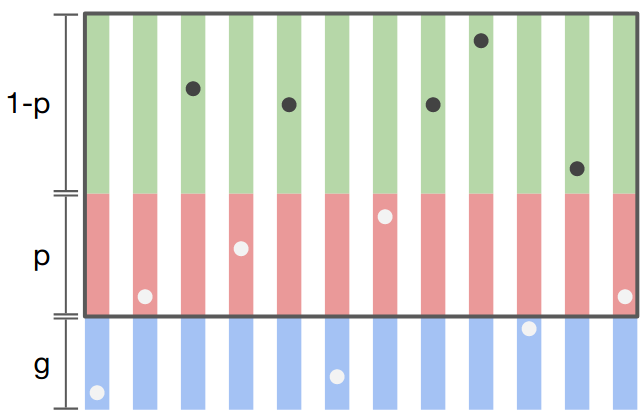
\includegraphics[height=4cm]{chernoff}
                \caption{\emph{
                    We randomly select points on $N$ vertical sticks.  Each
                    stick has three parts: \textbf{green} with length $1-p$,
                    \textbf{red} with length $p$, and \textbf{blue} with length
                    $g$.  We call non-blue points \textbf{boxed} and non-green
                    points \textbf{hollow}.
                    %
                    Shown are $9$ boxed points and $7$ hollow ones.
                }}
            \end{figure}

            We'll bound the chance that at least $M_0 = (p+g)N$ heads
            appear.  That is, we will bound the conditional probability ---
            given that all points are boxed --- that at least $M_0$
            points are red. 
            %
            For any $M\geq M_0$:
            \begin{align*}
                    & ~ \PP[\text{$M$ are red $\mid$ all are boxed}] \\
                  = & ~ \PP[\text{$M$ are red $\wedge$ all are boxed}] ~/~ 
                        \PP[\text{all are boxed}]  \\
                  = & ~ \PP[\text{$M$ are hollow $\wedge$ all hollows are red}] ~/~ 
                        \PP[\text{all are boxed}]  \\
                  = & ~ \PP[\text{$M$ are hollow}] \cdot
                        \PP[\text{all hollows are red $\mid$ $M$ are hollow}] ~/~
                        \PP[\text{all are boxed}] \\
                  = & ~ \PP[\text{$M$ are hollow}] \cdot (1+g/p)^{-M} ~/~ (1+g)^{-N}  \\
                \leq& ~ \PP[\text{$M$ are hollow}] \cdot (1+g/p)^{-M_0} ~/~ (1+g)^{-N} 
            \end{align*}
            Since the above holds for all $M\geq M_0$, we conclude:
            \begin{align*}
                ~   & ~ \PP[\text{at least $M_0$ are red $\mid$ all are boxed}] & \\
                %\leq& ~ \PP[\text{at least $M_0$ are hollow}] \cdot (1+g/p)^{-M_0} ~/~ (1+g)^{-N} \\
                \leq& ~ (1+g/p)^{-M_0} / (1+g)^{-N}             & \text{probabilities are at most $1$} \\
                \leq& ~ \exp(-M_0 g/p) \exp(Ng)                 & \text{$\exp$ is convex} \\ 
                =   & ~ \exp(-(p+g)N g/p + Ng) = \exp(-Ng^2/p)  & \text{$M_0=(p+g)N$} \\ 
                \leq& ~ \exp(-Ng^2)                             & \text{probabilities are at most $1$}
            \end{align*}
            This is \textbf{Chernoff's bound} for coin flips.
        \end{proof}

\end{document}
